\documentclass[12pt]{book}
\usepackage{geometry}                % See geometry.pdf to learn the layout options. There are lots.
\geometry{a4paper}                   % ... or a4paper or a5paper or ... 
%\geometry{landscape}                % Activate for for rotated page geometry
%\usepackage[parfill]{parskip}    % Activate to begin paragraphs with an empty line rather than an indent
\usepackage{graphicx}
\usepackage{amssymb}
\usepackage{amsmath}
\usepackage{epstopdf}
\usepackage{caption}
\usepackage{subcaption}
\usepackage[english]{babel}
\usepackage[T1]{fontenc}
\usepackage{epstopdf}
\usepackage[utf8]{inputenc}
\usepackage{units}
\usepackage[toc,page]{appendix}
\usepackage[section]{placeins}
\usepackage[percent]{overpic}
%\usepackage{titling}
\usepackage{cite}
\usepackage{nicefrac}
\usepackage{xcolor}
\usepackage{tikz}
\usepackage{standalone}
\usepackage{siunitx}
\usepackage{multirow}
\usepackage{booktabs}
\usetikzlibrary{shapes,arrows,calc,fadings}
\usetikzlibrary{trees}
\usetikzlibrary{shadows.blur}
\usetikzlibrary{positioning}
\usetikzlibrary{decorations.pathmorphing}
\usetikzlibrary{decorations.markings}
\usepackage{breakcites}


\newcommand \dd[1]  { \,\textrm d{#1}   }
\pagestyle{plain}

\usepackage{hyperref}
\usepackage{url}
\newcommand{\subtitle}[1]{%
  \posttitle{%
    \par\end{center}
    \begin{center}\large#1\end{center}
    \vskip0.5em}%
}
\RequirePackage{lineno}
\setlength{\linenumbersep}{6pt}
%\linenumbers

%\title{Jet quenching in fluctuating events in heavy-ion collisions}
%\title{Particle Identified Flow and Unfolding in Heavy Ion Collisions}
%\subtitle{Master's thesis}
%\author{Tomas Snellman}
%\date{}                                           % Activate to display a given date or no date


\def\fig#1{Fig.~\ref{#1}}
\def\eq#1{Eq.~(\ref{#1})}
\def\tab#1{Tab.~\ref{#1}}
\def\sec#1{Sec.~\ref{#1}}

\def\tev{\mbox{~TeV}}
\def\gevc{\mbox{~GeV/$c$}}
\def\gevcc{\mbox{~GeV/$c^2$}}
\def\mevc{\mbox{~MeV/$c$}}

\def\simge{\stackrel{>}{\sim} }
\def\simle{\stackrel{<}{\sim} }
%\def\la{\langle }
%\def\ra{\rangle }
\def\la{\left< }
\def\ra{\right> }
\def\mean#1{\ensuremath{\la#1\ra}}
\def\meanabs#1{\ensuremath{\la|#1|\ra}}
\def\meankv#1{\ensuremath{\la#1^2\ra}}
\def\rms#1{\meankv{#1}}
\def\sqrtrms#1{\ensuremath{\sqrt{\meankv{#1}}}}

\def\eg{{\it e.g.}}
\def\etc{{\it etc}}



\newcommand{\sqrtS}{\ensuremath{\sqrt{s}}}
\newcommand{\sqrtSnn}{\ensuremath{\sqrt{s_{\mathrm{NN}}}}}
\newcommand{\sqrtSE}[2][TeV]{\ensuremath{\sqrtS = #2~\mathrm{#1}}}
\newcommand{\sqrtSnnE}[2][TeV]{\ensuremath{\sqrtSnn = #2~\mathrm{#1}}}
\newcommand{\GeVc}{\ensuremath{\mathrm{GeV}\kern-0.05em/\kern-0.02em c}}
\newcommand{\gev}{\ensuremath{\mathrm{GeV}\kern-0.05em}}
\def\pt#1{\ensuremath{p_{\rm T#1}}} 
\def\jt#1{\ensuremath{j_{\rm T#1}}}
\def\vjt#1{\ensuremath{\vec{j}_{\rm T#1}}}
\def\kt#1{\ensuremath{k_{\rm T#1}}}
\newcommand{\xlong} {\ensuremath{x_{\parallel}}}
\def\mean#1{\left<#1\right>}
\def\rms#1{\ensuremath{\sqrt{\left<#1^2\right>}}}
\DeclareUnicodeCharacter{00A0}{ }



\newcommand{\sign} {\ensuremath{\sigma_{\rm N}}}
\newcommand{\siga} {\ensuremath{\sigma_{\rm A}}}
\newcommand{\yn} {\ensuremath{Y_{\rm N}}}
\newcommand{\yf} {\ensuremath{Y_{\rm F}}}
\newcommand{\cf}{\ensuremath{CF}}
\newcommand{\D} {\ensuremath{D^q_\pi}}
\newcommand{\Dz} {\ensuremath{D^h_q(z,Q^2)}}
\newcommand{\fq}{\ensuremath{f_Q(\hat{p}_T)}}
\newcommand{\sq}{\ensuremath{\Sigma_Q(\hat{p}_T)}}
\newcommand{\fkt}{\ensuremath{f^\prime_Q(\hat{p}_{\rm Tt})}}
\newcommand{\skt}{\ensuremath{\Sigma^\prime_Q(\hat{p}_{\rm Tt})}}
\newcommand{\prob}{\ensuremath{\mathcal{P}}}
\newcommand{\condta}{\ensuremath{\Big|_{\pt{t},\pt{a}}}}

\newcommand{\auau} {\ensuremath{Au+Au}}
\newcommand{\dau} {\ensuremath{d+Au}}
\newcommand{\pp}{\ensuremath{\mbox{p\kern-0.05em p}}}
\newcommand{\ppbar}{\ensuremath{\mathrm{p\kern-0.05em \bar{p}}}}
\newcommand{\ee} {\ensuremath{e^+ + e^-}}
\newcommand{\pbpb} {\ensuremath{Pb+Pb}}
\newcommand{\ppb} {\ensuremath{p+Pb}}
\newcommand{\pPb}{\ensuremath{\mbox{p--Pb}}}
\newcommand{\PbPb}{\ensuremath{\mbox{Pb--Pb}}}


\def\ptq#1{\ensuremath{\hat{p}_{\rm T#1}}} 
\def\ptqkv#1{\ensuremath{\hat{p}^2_{\rm T#1}}} 
\def\vptq#1{\ensuremath{\vec{\hat{p}}_{\rm T#1}}} 
\def\ptg{\ensuremath{p_{\rm T\gamma}}} 

\def\pt#1{\ensuremath{p_{\rm T#1}}} 
\def\ptkv#1{\ensuremath{p^2_{\rm T#1}}} 
\def\vpt#1{\ensuremath{\vec{p}_{\rm T#1}}} 

\def\kt#1{\ensuremath{k_{\rm T#1}}} 
\def\ktkv#1{\ensuremath{k^2_{\rm T#1}}} 
\def\vkt#1{\ensuremath{\vec{k}_{\rm T#1}}} 

\def\jt#1{\ensuremath{j_{\rm T#1}}} 
\def\jtkv#1{\ensuremath{j^2_{\rm T#1}}} 
\def\vjt#1{\ensuremath{\vec{j}_{\rm T#1}}} 

\def\mkv#1{\ensuremath{m^2_{#1}}}
\def\mt#1{\ensuremath{m_{\rm T#1}}}
\def\mtkv#1{\ensuremath{m^2_{\rm T#1}}}

\newcommand{\mpt} {\mean{\pt{}}} 
\newcommand{\ptt}{\ensuremath{p_{\rm Tt}}}
\newcommand{\mptt} {\mean{\ptt}} 
\newcommand{\pta}{\ensuremath{p_{\rm Ta}}}
\newcommand{\mpta} {\mean{\pta}} 
\def\pn{\ensuremath{\hat{p}_{\rm n}}} 
\def\pnkv{\ensuremath{\hat{p}^2_{\rm n}}} 
\def\vpn{\ensuremath{\vec{\hat{p}}_{\rm n}}} 

\newcommand{\pout} {\ensuremath{p_{\rm out}}}
\newcommand{\qout} {\ensuremath{\hat{p}_{\rm out}}}


\newcommand{\mz} {\mean{z}}
\newcommand{\zt} {\ensuremath{z_{\rm t}}}
\newcommand{\mzt} {\mean{\zt}}
\newcommand{\za} {\ensuremath{z_{\rm a}}}
\newcommand{\mza} {\mean{\za}}
\newcommand{\xe} {\ensuremath{x_{\rm E}}}
\newcommand{\xh} {\ensuremath{x_{\rm h}}}
\newcommand{\xhq} {\ensuremath{\hat{x}_{\rm h}}}
\newcommand{\zkt} {\ensuremath{ \mean{\zt}\sqrtrms{\kt{}} }}
\newcommand{\xzkt} {\ensuremath{ \xhq^{-1}\mean{\zt}\sqrtrms{\kt{}} }}
\newcommand{\xzktfull} {\ensuremath{ \xhq^{-1}(\kt{},\xh)\mean{\zt(\kt{},\xh)}\sqrtrms{\kt{}} }}

\newcommand{\zT} {\ensuremath{z_{\rm T}}}

\newcommand{\snn} {\ensuremath{\sqrt{s_{NN}}}}
\newcommand{\s} {\ensuremath{\sqrt{s}}}
\newcommand{\piz} {\ensuremath{\pi^0}}
\newcommand{\pizh}{\ensuremath{\pi^0-h^\pm}}
\newcommand{\gammah}{\ensuremath{\rm direct-\gamma-h^\pm}}
\newcommand{\pipmh}{\ensuremath{\pi^\pm-h^\pm}}
\newcommand{\hh}{\ensuremath{h^\pm-h^\pm}}

\newcommand{\pbar} {\ensuremath{\overline{p}}}
\newcommand{\lbar} {\ensuremath{\overline{\Lambda}}}
\newcommand{\ntrig} {\ensuremath{N_{\rm trig}}}
\newcommand{\npart} {\ensuremath{N_{\rm part}}}
\newcommand{\npartav} {\ensuremath{\la N_{\rm part} \ra}}
\newcommand{\ncoll} {\ensuremath{N_{\rm coll}}}
\newcommand{\ncollav} {\ensuremath{\la N_{\rm coll} \ra}}
\newcommand{\ut} {\ensuremath{\la u_t \ra}}

\newcommand{\alphas} {\ensuremath{\alpha_{s}}}
\newcommand{\alphasQ} {\ensuremath{\alpha_{s}(Q^2)}}
\newcommand{\alphasQsqr} {\ensuremath{\alpha_{s}^2(Q^2)}}
\newcommand{\alphaqedQ} {\ensuremath{\alpha_{EM}(Q^2)}}
\newcommand{\SUT} {\ensuremath{SU(3)}}
\newcommand{\dphi} {\ensuremath{\Delta \phi}}
\newcommand{\xt} {\ensuremath{x_{\rm T}}}
\newcommand{\xtt} {\ensuremath{x_{\rm Tt}}}
\newcommand{\rmskt} {\ensuremath{ \sqrt{\mean{{\kt{}^2}} }}}

\newcommand{\spn} {\ensuremath{\sigma}}
\newcommand{\ptaf} {\ensuremath{\mathbf{\ptq{a}}}}
\newcommand{\pttf} {\ensuremath{\mathbf{\ptq{t}}}}

\def\etall{{\it et al.}}

\begin{document}

%!TEX root = Thesis.tex


%%%%%%%%%%%%%%%%%%%%%%%%%%%%%%%%%%%%%%%%%%%%%%%%
%                            Front (Title) page
%%%%%%%%%%%%%%%%%%%%%%%%%%%%%%%%%%%%%%%%%%%%%%%%

\thispagestyle{empty}
\vspace*{10mm}

\centerline{DEPARTMENT OF PHYSICS, UNIVERSITY OF JYV\"ASKYL\"A}
\centerline{RESEARCH REPORT No. ??/2019}

\vspace{25mm} 

\centerline{\bf JET TRANSVERSE MOMENTUM DISTRIBUTIONS }
\centerline{\bf  FROM RECONSTRUCTED JETS}

\centerline{\bf  IN P--PB COLLISIONS AT \sqrtSnnE{5.02}}
\centerline{\bf }

\vspace{13mm}


\centerline{\bf BY}
\centerline{\bf TOMAS SNELLMAN}

\vspace{13mm}

\centerline{Academic Dissertation}
\centerline{for the Degree of}
\centerline{Doctor of Philosophy}

\vspace{13mm}

%\centerline{To be presented, by permission of the}
%\centerline{Faculty of Mathematics and Natural Sciences}
%\centerline{of the University of Jyv\"askyl\"a,}
%\centerline{for public examination in Auditorium FYS 1 of the}
%\centerline{University of Jyv\"askyl\"a on MONTH DATE, YEAR,}
%\centerline{at 12 o'clock noon}

\vspace{13mm}



%\centerline{\picture{19mm}{50mm}{Soihtu}}

\centerline{Jyv\"askyl\"a, Finland}
%\centerline{\today}
\centerline{June 2019}

%%%%%%%%%%%%%%%%%%%%%%%%%%%%%%%%%%%%%%%%%%%%%%%%
%                            Author page
%%%%%%%%%%%%%%%%%%%%%%%%%%%%%%%%%%%%%%%%%%%%%%%%
\pagebreak
\thispagestyle{empty}

\vspace*{25mm} 

\begin{table}[h!]
%\centering
  \begin{tabular}{ p{4cm}  p{6cm} }
  {\bf Author} 	& {Tomas Snellman}\\  
  {} 			& {University of Jyv\"askyl\"a}\\  
  {} 			& {Finland}\\  
  {} 			& {}\\  

  {\bf Supervisors} 	& {Dr.~Kim Dong Jo}\\  
  {} 				& {University of Jyv\"askyl\"a}\\  
  {} 				& {Finland}\\  
  {} 				& {}\\  

  {}			 	& {Prof.~Jan Rak}\\  
  {} 				& {University of Jyv\"askyl\"a}\\  
  {} 				& {Finland}\\  
  {} 				& {}\\  

  {\bf Reviewers} 	& {Prof.~Stefan Bathe}\\  
  {} 				& {Baruch College, CUNY}\\  
  {} 				& {USA}\\  
  {} 				& {}\\  

  {}			 	& {Prof.~Marcin Chrząszcz}\\  
  {} 				& {Instytut Fizyki Jądrowej PAN}\\  
  {} 				& {Poland}\\  
  {} 				& {}\\  
    
  {\bf Opponent} 	& {Prof.~Jamie Nagle}\\  
  {} 				& {University of Colorado Boulder}\\  
  {} 				& {USA}\\  
  {} 				& {}\\  

  \end{tabular}
  \label{}
\end{table}
\pagebreak
%%%%%%%%%%%%%%%%%%%%%%%%%%%%%%%%%%%%%%%%%%%%%%%%%
%%                            Dedication page
%%%%%%%%%%%%%%%%%%%%%%%%%%%%%%%%%%%%%%%%%%%%%%%%%
%
%\vspace*{10mm} 
%\thispagestyle{empty}
%\begin{flushright}
%\end{flushright}
%\pagebreak
%%%%%%%%%%%%%%%%%%%%%%%%%%%%%%%%%%%%%%%%%%%%%%%%%
%%                            An empty page
%%%%%%%%%%%%%%%%%%%%%%%%%%%%%%%%%%%%%%%%%%%%%%%%%
%\thispagestyle{empty}
%\mbox{} 
%\pagebreak
%%%%%%%%%%%%%%%%%%%%%%%%%%%%%%%%%%%%%%%%%%%%%%%%
%                           Start page numbering
%%%%%%%%%%%%%%%%%%%%%%%%%%%%%%%%%%%%%%%%%%%%%%%%
\pagenumbering{roman}
\setcounter{page}{1}

%\cleardoublepage
\section*{Acknowledgements} 
\label{acknowledgment}
\pagenumbering{arabic}
\setcounter{page}{0}
%\maketitle
% !TEX root = thesis.tex

%\section{Introduction}

\begin{abstract}

\end{abstract}
\tableofcontents
%\listoffigures

\clearpage
\section{Introduction}
{\color{red} REWRITE
 At sufficiently high energies quarks and gluons are no longer bound to hadrons, but they form a deconfined state known as Quark-Gluon plasma (QGP). The main goal of heavy-ion physics is the study of QGP and its properties.
One of the experimental observables that is sensitive to the properties of QGP is the azimuthal distribution of particles in the plane perpendicular to the beam direction. 

When nuclei collide at non-zero impact parameter (non-central collisions), their overlap region is asymmetric. This initial spatial asymmetry is converted via multiple collisions into an anisotropic momentum distribution of the produced particles. For low momentum particles ($\pt{} \lesssim 3$ \gevc), this anisotropy is understood to result from hydrodynamically driven flow of the QGP~\cite{Adcox:2004mh, Adams:2005dq, Ollitrault:1992, Heinz:2002, Shuryak:2009}. 

One way to characterize this anisotropy is with coefficients from a Fourier series parametrization of the azimuthal angle distribution of emitted hadrons. The second order coefficient, $v_2$ which is also known as elliptic flow, shows clear dependence on centrality. The collision geometry is mainly responsible for the elliptic flow. Higher harmonics don't depend that much on centrality. These higher harmonics carry information about the fluctuations in collisions. The event-by-event fluctuations have an increasing importance in measurements and it has been observed that measurements of elliptic flow in central collisions and measurements of higher order harmonics are consistent with the assumption that flow in these cases is mainly due to fluctuations~\cite{Jia:2012ve}.



At LHC energies  $\sqrt{s_{NN}}=2.76\mathrm{GeV}$ it has been observed that in general there is little difference to flow at RHIC energies. The $v_2$ coefficient is about 20\% greater at LHC than at RHIC, depending on the centrality bin. 
The particle identified $v_2$ for kaons and pions follows the same trend. However it was observed that for proton $v_2$ the quark number scaling does not work~\cite{Lacey:2012ma}. So far there is no agreement of why this scaling breaks down at LHC or why it works so well at RHIC energies.
}


\pagebreak
\subsection{Quantum chromodynamics}
\subsubsection{Foundation of QCD}
There are four known basic interactions in the universe: gravity, electromagnetic, weak and strong interactions. The standard model of particle physics includes three of these, excluding the gravitational interaction. The theory of strong interactions is known as Quantum Chromodynamics (QCD).

The development of QCD began after the introduction of new powerful particle accelerators that were capable of particle physics research in the 1950s. Before this particles were mainly discovered from cosmic rays. Positrons, neutrons and muons were discovered in the 1930s and charged pions were discovered in 1947~\cite{Occhialini:1987nr,Lattes:1947mx}. The neutral pion was discovered in 1950~\cite{Bjorklund:1950}.

The Lawrence Berkeley National Laboratory started the Bevalac accelerator in 1954, Super Proton Synchrotron (SPS) in CERN began operating in 1959 and the Alternating Gradient Synchrotron (AGS) at Brookhaven started in 1960. With an energy of \unit[33]{\gev} AGS was the most powerful accelerator of that time. By the beginning of 1960s several new particles had been discovered. These included antiprotons~\cite{Chamberlain:1955ns}, antineutrons~\cite{Cork:1957nu}, $\Delta$-particles and the six hyperons ($\Xi^0$\cite{Alvarez:1959zz}, $\Xi^-$~\cite{Armenteros:1952nt}, $\Sigma^{\pm}$~\cite{Bonetti1953}, $\Sigma^0$~\cite{Plano1957} and $\Lambda$~\cite{Fowler:1953qpk}).

Facing this avalanche of new particles, physicists started the search for symmetries within them. Already in 1932 Heisenberg~\cite{Heisenberg:1932} 
had proposed an isospin model to explain similarities between the proton and the neutron. In 1962 Gell-Mann and Ne'eman presented that particles sharing the same quantum numbers (spin, parity) could be organised using the symmetry of SU(3).~\cite{Gell-Mann:1962} Heisenberg's Isospin model followed the symmetry of SU(2). Using the SU(3) model known baryons and mesons could be presented as octets. This also lead to the discovery of the $\Omega^{-}$~\cite{Barnes:1964ga} particle since this was missing from the SU(3) decouplet that included heavier baryons. 

The most simple representation of SU(3) was a triplet. Inside this triplet particles would have electric charges $\nicefrac{2}{3}$ or $-\nicefrac{1}{3}$. However, these had not been detected. In 1964 Gell-Mann~\cite{Gell-Mann:1964} and Zweig~\cite{Zweig:1964jf} proposed that baryons and mesons would be bound states of these three hypothetical triplet particles that Gell-Mann called quarks. Zweig's nomenclature, aces, didn't live on. Now we know that these are the $u$, $d$ and $s$ quarks. However, this original quark model without colour was violating the Pauli exclusion principle. For example the $\Omega^{-}$ particle is comprised of three $s$ quarks, two of which would have exactly the same quantum states, since spin can only have two values. 

First experimental indication of the existence of these quarks came in 1969 when a series of experiments at the Stanford Linear Accelerator Center (SLAC) revealed that protons and neutrons appeared to have some substructure~\cite{Bloom:1969kcm, Breidenbach:1969kd}. Bjorken demonstrated that these results could be explained if protons and neutrons were composed of virtually noninteracting pointlike particles~\cite{Bjorken:1968dy,Bjorken:1969ja}. Feynman~\cite{Feynman:1969ej} interpreted these objects as real particles and suggested they would be the quarks of Gell-Mann's model. At the time, however, this was mysterious; if all strongly interacting particles, hadrons, were composed of quarks, then quarks should surely be strongly interacting themselves. Why would they appear to be almost free inside hadrons?~\cite{Krauss:2017}

The idea of colour had already been presented by Greenberg in 1964~\cite{Greenberg:1964}. In 1971 Gell-Mann and Fritzsch presented their model~\cite{Fritzsch:1972jv}, which solved the antisymmetry problem. They added a colour quantum number to quarks, which separated quarks of the same species. In the new colour model the baryonic wave function became

\begin{equation}
\left( qqq\right)\rightarrow\left(q_rq_gq_b-q_gq_rq_b+q_bq_rq_g-q_rq_bq_g+q_gq_bq_r-q_bq_gq_r\right),
\end{equation}


%improve
\noindent The colour model was also supported by experimental evidence. The decay rate of a neutral pion with the addition of colours is

\begin{equation}
\Lambda\left(\pi^0\rightarrow\gamma \gamma\right) = \frac{\alpha^2}{2\pi}\frac{N_c^2}{3^2}\frac{m_\pi^3}{f_\pi^2}.
\end{equation} 

\noindent For $N_c=3$ this gives \unit[7.75]{eV} and the measured value is $(7.86\pm0.54)\,\mathrm{eV}$~\cite{Williams:1988sg}.

Another observable that combines the colour information also to the number of quark flavours is the Drell-Ratio $R$~\cite{Krolikowski:1974jx}

\begin{equation}
R=\frac{\sigma\left(e^++e^-\rightarrow\mathrm{hadrons}\right)}{\sigma\left(e^++e^-\rightarrow\mu^++\mu^-\right)}=N_c\sum_fQ_f^2.
\end{equation}

\noindent This ratio has the numerical value 2 when including the three light quarks $u$, $d$ and $s$. When the collision energy reaches the threshold of heavy quark ($c$ and $b$) production processes this increases to $\nicefrac{10}{3}$ (for $f=u,d,s,c$) and \nicefrac{11}{3} (for $f=u,d,s,c,b$). The energy threshold ($\sqrt{s}\approx350\gev$) of $t\bar t$ production, has not been reached so far by any $e^+e^-$ colliders.

%\cite{Glashow:1970gm} Introduction of lepton-quark symmetry by Glashow,Iliopoulos and Maiani, proposal of a fourth (charmed) quark.
%\\cite{Bacci:1974za} ADONE Discovery of charm quark and $J/\Psi$
%\cite{Aubert:1974js} BNL
%\cite{Augustin:1974xw} SLAC

The quark model was extended in 1974 when the discovery of the charm quark and the first charmed hadron, $J/\Psi$, was simultaneously published by teams from the SLAC~\cite{Augustin:1974xw}, from Brookhaven National Laboratory~\cite{Aubert:1974js} and from the ADONE collider in Frascati, Italy~\cite{Bacci:1974za}. The existence of a fourth quark was already speculated in 1964 by Bjorken and Glashow~\cite{Bjorken:1964gz}, but a proper prediction was provided by Glashow, Iliopoulos and Maiani in 1970~\cite{Glashow:1970gm} based on symmetries between leptons and quarks in weak interactions.


The colour model explained why no free quarks had been observed as only colour neutral states are possible. The simplest ways of producing a colour neutral object are the combination of three quarks, and the combination of a quark-antiquark pair. These are known as baryons and mesons.

After the addition of colour the main ingredients of QCD had been established. The final quantum field theory of Quantum Chromodynamics formed quickly between 1972 and 1974. Main part of this was the work by Gross, Wilczek, Politzer and George for non-abelian gauge field theories~\cite{gross1973ultraviolet, politzer1973reliable, gross1973asymptotically, gross1974asymptotically, georgi1974electroproduction}. Gross, Wilczek and Politzer received the Nobel Prize in Physics for their work~\cite{Nobel2004}. The role of gluons as a colour octet was presented by Fritzsch, Gell-Mann and Leutwyler in 1973~\cite{fritzsch1973advantages}. The theory had now 8 massless gluons to mediate the strong interaction.

However, these gluons had not been discovered. Indirect evidence of the existence had been seen as it was observed that only about half of the momentum of protons was transported by the quarks~\cite{25gluons}. Direct evidence should be seen in electron-electron collisions as a third, gluonic, jet in addition to two quark jets. Three jet events were first seen in 1979 at the PETRA accelerator at DESY~\cite{Brandelik1979243, PhysRev.43.830, Berger1979418}.

\subsubsection{Asymptotic Freedom}
In Quantum Electrodynamics (QED) the electric charge is screened. In the vicinity of a charge, the vacuum becomes polarized. Virtual charged particle-antiparticle pairs around the charge are arranged so that opposing charges face each other. Since the pairs also include an equal amount opposite charge compared to the original charge the average charge seen by an observer at a distance is smaller. When the distance to the charge increases the effective charge decreases until the coupling constant of QED reaches the fine-structure constant $\alpha=\frac{1}{137}$.~\cite{Perkins:1982xb}

Contrary to QED, QCD is a non-abelian theory. In other words the generators of the symmetry group of QCD, SU(3), do not commute. This has the practical consequence that gluons interact also with other gluons, whereas in QED the neutral carrier particles, photons, only interact with charged particles.
There is screening also in QCD because of the colour charges, but in addition to that there is antiscreening because of the gluon interactions. In QCD the antiscreening effect dominates over screening. Thus for larger distances to the colour charge the coupling constant is larger. This explains why no free colour charges can be observed. When the distance between charges increases the interaction strengthens until it is strong enough to produce a new quark-antiquark pair. On the other hand, at very small distances the coupling constant approaches zero. This is called asymptotic freedom.~\cite{Perkins:1982xb}

In 1975 Collins\cite{Collins:1975} predicted a state where individual quarks and gluons are no longer confined into bound hadronic states. Instead they form a bulk QCD matter that Edward Shuryak called Quark-Gluon plasma in his 1980 review of QCD and the theory of superdense matter~\cite{Shuryak:1980}. QGP can be seen as a separate state of matter. A schematic view of a phase diagram for QCD matter is shown in Fig. \ref{fig:QCDphase}. 

\begin{figure}[htbp]
\centering
%\includegraphics[width=0.9\textwidth]{pics/qcd_ms_high}
\includegraphics[width=0.5\textwidth]{pics/QCDphase2.pdf}
\caption[QCD phase diagram]{A schematic outline for the phase diagram of QCD matter at ultra-high density and temperature. The quark chemical potential $\mu$ that is on the x-axis represents the imbalance between quarks and antiquarks. At zero temperature this corresponds to the number of quarks but at higher temperatures there are also additional pairs of quarks and antiquarks. Along the horizontal axis the temperature is zero, and the density is zero up to the onset transition where it jumps to nuclear density, and then rises with increasing $\mu$.  Neutron stars are in this region of the phase diagram, although it is not known whether their cores are dense enough to reach the quark matter phase. Along the vertical axis the temperature rises, taking us through the crossover from a hadronic gas to the quark-gluon plasma. This is the regime explored by high-energy heavy-ion colliders.~\cite{Rajagopal:2001}}
\label{fig:QCDphase}
\end{figure}


In the early universe at the age of $10^{-6}\mathrm{s}$ after the Big Bang the conditions preferred the existence of QGP instead of hadronic matter. Nowadays bulk QCD matter, its properties and its phase transitions between hadronic matter and the quark-gluon plasma (QGP) can be explored in the laboratory, through collisions of heavy atomic nuclei at ultra-relativistic energies. The study of QCD matter at high temperature is of fundamental and broad interest. The phase transition in QCD is the only phase transition in a quantum field theory that can be probed by any present or foreseeable technology. 

One important property of the QGP is the shear viscosity to entropy ratio, $\nicefrac{\eta}{s}$. It is believed that this ratio has an universal minimum value of $\nicefrac{1}{4\pi}\approx 0.08$, among all substances in nature. This limit would be reached in the strong coupling limit of certain gauge theories~\cite{Kovtun:2004de}. The temperature dependance of the ratio is shown in Fig. \ref{fig:etas}. The minimum value of $\nicefrac{\eta}{s}$ is found in the vicinity of the critical temperature, $T_c$~\cite{PhysRevLett.98.092301}. Finding the $\nicefrac{\eta}{s}$ values in QGP matter would therefore also provide a way of determining the critical point of QCD matter.

The $\nicefrac{\eta}{s}$ value for the matter created in Au-Au collisions at RHIC ($\sqrt{s_{NN}}=\unit[200]{\gev}$)  has been estimated to be $0.09\pm0.015$~\cite{PhysRevLett.98.092301}, which is very close to the lowest value for a wide class of thermal quantum field theories~\cite{Kovtun:2004de} for all relativistic quantum field theories at finite temperature and zero chemical potential. This suggests that the the matter created goes through a phase where it is close to the critical point of QCD.

\begin{figure}[htb]
\centering
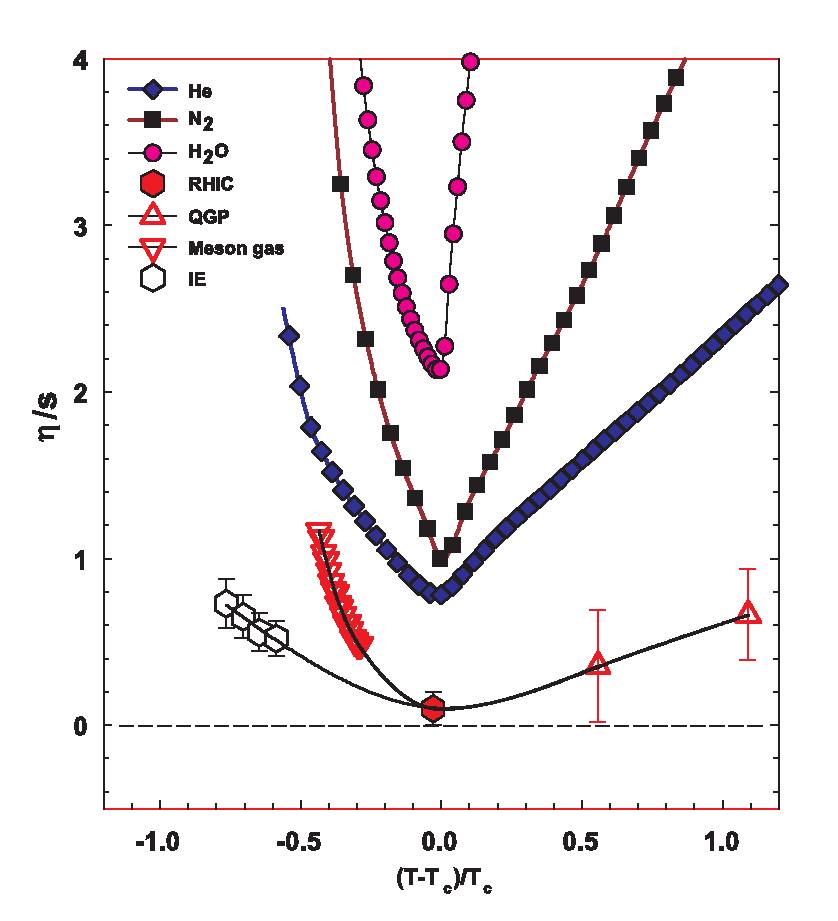
\includegraphics[width=0.5\textwidth]{pics/eta-s-vs-t-tc3}
\caption[$\eta/s$ vs $(T-T_c)/T_c$]{\label{fig3}$\eta/s$ as a function of $(T-T_c)/T_c$ for several substances as indicated. The $\nicefrac{\eta}{s}=0.09\pm0.015$ estimate at RHIC comes from Au-Au collisions at $\sqrt{s_{NN}}=\unit[200]{\gev}$. 
	The calculated values for the meson-gas have an associated error 
	of $\sim$ 50\% %~\cite{Chen:2006ig}. 
	The lattice QCD value $T_c = 170$~MeV %~\cite{Karsch:2000kv} 
	is assumed for nuclear matter. The lines are drawn to guide the eye.~\cite{PhysRevLett.98.092301}
}
\label{fig:etas}
\end{figure}



\FloatBarrier
\pagebreak
\subsection{heavy-ion physics}
The Quark Gluon Plasma (QGP) is experimentally accessible by colliding heavy-ions at high energies. Nowadays research of Heavy-Ion Collisions is mainly performed at two particle colliders; The Relativistic heavy-ion Collider (RHIC) at BNL in New York, USA and he Large Hadron Collider (LHC) at CERN in Switzerland. Energy densities at these colliders should be enough to produce QGP and convincing evidence of the creation has been seen at both colliders. Complimentary research with heavy nuclei is also performed at the Super Proton Synchrotron (SPS) at CERN.

The development of heavy-ion physics is strongly connected to the development of particle colliders. Experimental study of relativistic heavy-ion collisions has been carried out for three decades, beginning with the Bevalac at Lawrence Berkeley National Laboratory (LBNL)~\cite{Lofgren_1975}, and continuing with the AGS at Brookhaven National Laboratory (BNL)~\cite{Barton:1987}, CERN SPS~\cite{Vitev:2002pf}, RHIC at BNL and LHC at CERN. 

%The first colliders could not produce enough energy to create QGP matter so they could only probe the hadronic state. 
%
%The collective motion of matter in a heavy-ion collision has been modeled using several models e.g. the Blast wave Model~\cite{PhysRevC.84.064905} has been used succesfully. Another model growing in popularity is the hydrodynamical approach which is further discussed in section \ref{sec:hydro}.

\subsubsection{History}
The first heavy-ion collisions were performed at the Bevalac experiment at the Lawrence Berkeley National Laboratory~\cite{Lofgren_1975} and at the Joint Institute for Nuclear Research in Dubna~\cite{kovalenko1994status} at energies up to 1$\gev$ per nucleon.
In 1986 the Super Proton Synchrotron (SPS) at CERN started to look for QGP signatures in O+Pb collisions. The center-of-mass energy per colliding nucleon pair $\left(\sqrt{s_{NN}}\right)$ was \unit[19.4]{GeV}~\cite{Vitev:2002pf}. These experiments did not find any decisive evidence of the existence of QGP. In 1994 a heavier lead (Pb) beam was introduced for new experiments at $\sqrt{s_{NN}}\approx \unit[17]{\gev}$. At the same time the Alternating Gradient Synchrotron (AGS) at BNL, Brookhaven collided ions up to $\mathrm{^{32}S}$ with a fixed target at energies up to \unit[28]{\gev}~\cite{Barton:1987}. In 2000 CERN~\cite{SPSpress} presented compelling evidence for the existence of a new state of matter. Now SPS is used with 400 GeV proton beams for fixed-target experiments, such as the SPS heavy-ion and Neutrino Experiment (SHINE)~\cite{Grebieszkow:2013nza}, which tries to search for the critical point of strongly interacting matter.

The Relativistic heavy-ion Collider (RHIC) at BNL in New York, USA started its  operation in 2000. The top center-of-mass energy per nucleon pair at RHIC, \unit[200]{\gev}, was reached in the following years. The results from the experiments at RHIC have provided a lot of convincing evidences that QGP was created~\cite{Adcox:2004mh, Adams:2005dq, Arsene:2004fa, Back:2004je}. The newest addition to the group of accelerators capable of heavy-ion physics is the Large Hadron Collider (LHC) at CERN, Switzerland. LHC started operating in November 2009 with proton-proton collisions. First Pb-Pb heavy-ion runs started in November 2010 with $\sqrt{s_{NN}}=2.76\; \mathrm{TeV}$,  over ten times higher than at RHIC. Since then LHC has provided both \PbPb and \pPb collisions and a short period of XeXe collisions. Table~\ref{tab:datasets} shows a summary of these. Among the six experiments at LHC, the Large Ion Collider Experiment (ALICE) is dedicated to heavy-ion physics. Also CMS and ATLAS have active heavy-ion programs and LHCb uses its SMOG~\cite{Maurice:2017iom} to perform unique fixed target collisions with heavy ions. 


\begin{table}[htb]
\centering
\caption{Summary of datasets. The integrated luminosities are from ALICE.}
\label{tab:datasets}
\begin{tabular}{| c | S | c |}
\hline
\multicolumn{3}{| c |}{Run 1 (2009-2013)} \\
\hline
\multirow{4}{*}{\pp} & 0.9 \tev & $\sim \unit[200]{\mu b^{-1}}$ \\
 & 2.76 \tev & $\sim \unit[100]{n b^{-1}}$ \\
 & 7.0 \tev & $\sim \unit[1.5]{p b^{-1}}$ \\
 & 8.0 \tev & $\sim \unit[2.5]{p b^{-1}}$ \\
 \hline
\pPb & 5.02 \tev & $\sim\unit[15]{n b^{-1}}$ \\
\hline
\PbPb & 2.76 \tev & $\sim \unit[75]{\mu b^{-1}}$ \\
\hline
\end{tabular}
\begin{tabular}{| c | S | c |}
\hline
\multicolumn{3}{| c |}{Run 2 (2015-2018)} \\
\hline
\multirow{2}{*}{\pp} & 5.02 \tev & $\sim \unit[1.3]{p b^{-1}}$ \\
 & 13.0 \tev & $\sim \unit[25]{p b^{-1}}$ \\
 \hline
\multirow{2}{*}{\pPb} & 5.02 \tev & $\sim\unit[3]{n b^{-1}}$ \\
& 8.16 \tev & $\sim\unit[25]{n b^{-1}}$ \\
\hline
XeXe & 5.44 \tev & $\sim \unit[0.3]{\mu b^{-1}}$ \\
\hline
\PbPb & 5.02 \tev & $\sim \unit[1]{n b^{-1}}$ \\
\hline
\end{tabular}
\end{table}

\pagebreak
\FloatBarrier
%\pagebreak
\subsection{Features of Heavy-Ion Collisions}
\label{sec:features}
\subsubsection{Collision Geometry}
In contrast to protons atomic nuclei are objects with considerable transverse size. The properties of a heavy-ion collision depend strongly on the impact parameter $\vec b$ which is the vector connecting the centres of the two colliding nuclei at their closest approach. One illustration of a heavy-ion collision is shown in Fig.~\ref{fig:planes}.


Impact parameter defines the reaction plane which is the plane spanned by $b$ and the beam direction. $\Psi_{RP}$ gives the angle between the reaction plane and some reference frame angle. Experimentally the reference frame is fixed by the detector setup. Reaction plane angle cannot be directly measured in high energy nuclear collisions, but it can be estimated with the event plane method~\cite{Voloshin:2008dg}. 
\begin{figure}[h!]
\centering
\includegraphics[width=0.6\textwidth]{pics/Definitions}
\caption[The definitions of the Reaction Plane and Participant Plane coordinate systems]{The definitions of the Reaction Plane and Participant Plane coordinate systems~\cite{Voloshin:2007pc}. The dashed circles represent the two colliding nuclei and the green dots are partons that take part  in the collision. $x_{PP}$ and $x_{RP}$ are the participant and reaction planes. The angle between $x_{RP}$ and $x_{PP}$ is given by Eq. (\ref{eq:partangle}). $y_{PP}$ and $y_{RP}$ are lines perpendicular to the participant and reaction planes. }
\label{fig:planes}
\end{figure}


%The constituents in the nucleus have a quantum character and are situated in a potential well. 
%Nucleus density
%This causes fluctuations in the initial geometry of the overlapping region. 
Participant zone is the area containing the participants. The distribution of nucleons in the nucleus exhibits time-dependent fluctuations. Because the nucleon distribution at the time of the collision defines the participant zone, the axis of the participant zone fluctuates and can deviate from the reaction plane. The angle between the participant plane and the reaction plane is defined by ~\cite{Holopainen:2010gz}

\begin{equation}
\psi_{PP}=\arctan \frac{-2\sigma_{xy}}{\sigma_y^2-\sigma_x^2+\sqrt{\left(\sigma_y^2-\sigma_x^2\right)^2+4\sigma_{xy}^2}},
\label{eq:partangle}
\end{equation}

\noindent where the $\sigma$-terms are averaged over the energy density.

\begin{equation}
\sigma_y^2=\langle y^2\rangle-\langle y \rangle ^2, \sigma_x^2=\langle x^2\rangle-\langle x \rangle ^2, \sigma_{xy}=\langle xy \rangle - \langle x \rangle \langle y \rangle
\end{equation}

The impact parameter is one way to quantize the centrality of a heavy-ion collision but it is impossible to measure in a collision. It can be estimated from observed data using theoretical models, but this is always model-dependent and to compare results from different experiments one needs an universal definition for centrality. %The difference between central and peripheral collisions is illustrated in Fig.~\ref{fig:collisionA}. In a central collision the overlap region is larger than in a peripheral collision. Larger overlap region translates into a larger number of nucleons participating in the collision, which in turn leads to a larger number of particles produced in the event.


\begin{figure}[h!]
\centering
        \begin{subfigure}[b]{0.45\textwidth}
                \centering
            	\includegraphics[height=1in]{pics/Collisionperipheral}
                \caption{Peripheral collision}
                \label{fig:peripheral}
        \end{subfigure}
        \begin{subfigure}[b]{0.45\textwidth}
                \centering
               \includegraphics[height=1in]{pics/Collisioncentral}
                \caption{Central collision}
                \label{fig:central}
        \end{subfigure}
        \caption[Interaction between partons in central and peripheral collisions.]{Interaction between partons in central and peripheral collisions. The snowflakes represent elementary parton-parton collisions. When the impact parameter $b$ is large the number of elementary collisions is small. Particle production is small. Smaller impact parameter increases the number of elementary collisions. This increases  particle production.}\label{fig:collisionA}
\end{figure}

Instead in practice centrality is defined by dividing collision events into percentile bins by the number participants or experimentally by the observed multiplicity. Centrality bin 0-5\% corresponds to the most central collisions with the highest multiplicity and higher centrality percentages correspond to more peripheral collisions with lower multiplicities. A multiplicity distribution from ALICE measurements~\cite{PhysRevC.88.044909} illustrating the centrality division is shown in Fig.~\ref{fig:centrality}. The distribution is fitted using a phenomenological approach based on a Glauber Monte Carlo~\cite{Miller:2007ri} plus a convolution of a model for the particle production and a negative binomial distribution. 


\begin{figure}[htb]
\centering

               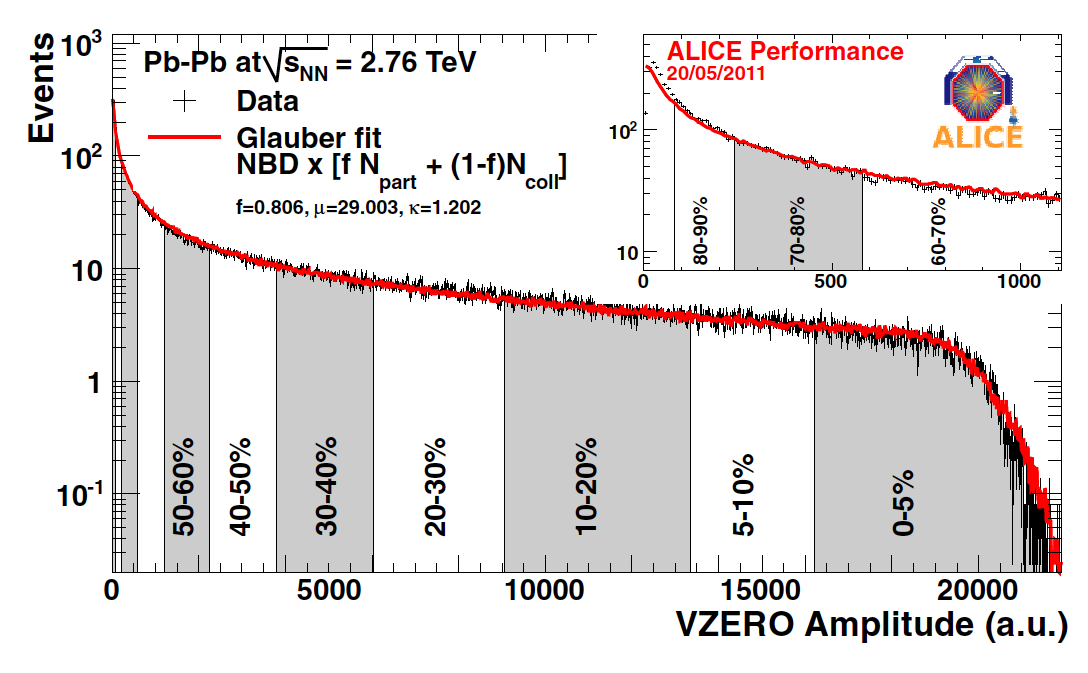
\includegraphics[width=0.9\textwidth]{pics/centrality.png}
        \caption[An illustration of the multiplicity distribution in ALICE measurement with centrality classes.]{An illustration of the multiplicity distribution in ALICE measurements. The red line shows
the fit of the Glauber calculation to the measurement. The data is divided into centrality bins~\cite{PhysRevC.88.044909}. The size of the bins corresponds to the indicated percentile.}
        	\label{fig:centrality}
\end{figure}

%Each centrality bin is obtained by taking the indicated percentile of events arranged by the observed multiplicity. 
%Centrality bin 0-5\% corresponds to the most central collisions. It includes the 5\% of the events  with highest multiplicity. Centralities 90-100\% correspond to the most peripheral collisions. 


%\subsubsection{Nuclear Geometry}
%\label{sec:glauber}
%To model heavy-ion collisions one must first have a description as good as possible of the colliding objects. Atomic nuclei are complex ensembles of nucleons. The nuclei used in heavy-ion physics have in the order of 200 nucleons. Mostly used nuclei are $\mathrm{^{208}Pb}$ at LHC and $\mathrm{^{197}Au}$ at RHIC. The distribution of these nucleons within a nucleus is not uniform and is subject to fluctuations in time.

\subsubsection{Glauber Model}
\label{sec:glauber}
Nuclear geometry in heavy-ion collisions is often modelled with the Glauber Model. The model was originally developed to address the problem of high energy scattering with composite particles. Glauber presented his first collection of papers and unpublished work in his 1958 lectures~\cite{Glauber:1959}. In the 1970's Glauber's work started to have utility in describing total cross sections, after Maximon and Czyz applied it to proton-nucleus and nucleus-nucleus collisions in 1969~\cite{Czyz:1969}. 

In 1976 ~\cite{Biallas1976461} Białłas, Bleszyński, and Czyż applied Glauber's approach to inelastic nuclear collisions. Their approach introduced the basic functions used in modern language including the thickness function and the nuclear overlap function. Thickness function is the integral of the nuclear density over a line going through the nucleus with minimum distance $s$ from its center

\begin{equation}
T_A\left(s\right)=\int_{-\infty}^{\infty}\dd z \rho\left(\sqrt{s^2+z^2}\right).
\end{equation}

\noindent This function gives the thickness of the nucleus, i.e. the amount material seen by a particle passing through it. 

Overlap function is an integral of the thickness functions of two colliding nuclei over the overlap area. This can be seen as the material that takes part in the collision. It is given as a function of the impact parameter $b$

\begin{equation}
T_{AB}\left(\vec b\right)=\int \dd{^2s} T_A\left(\vec s\right) T_B\left(\vec s - \vec b\right)
\end{equation}

\noindent The average overlap function, $\left<T_{AA}\right>$, in an A-A collisions  is given by~\cite{Afanasiev:2009aa}

\begin{equation}
\left<T_{AA}\right>=\frac{\int T_{AA}\left(b\right) \dd b}
{\int\left(1-e^{-\sigma^{inel}_{pp}T_{AA}\left(b\right)}\right)\dd b}.
\end{equation}

\noindent Using $\left<T_{AA}\right>$ one can calculate the mean number of binary collisions

\begin{equation}
\left<N_{coll}\right>=\sigma_{pp}^{inel}\left<T_{AA}\right>,
\end{equation}

\noindent where the total inelastic cross-section, $\sigma_{pp}^{inel}$, gives the probability of two nucleons interacting. The number of binary collisions is related to the hard processes in a heavy-ion collision. Each binary collision has equal probability for direct production of high-momentum partons. Thus the number of high momentum particles is proportional to $\left<N_{coll}\right>$~\cite{Abelev:2013qoq,Kharzeev:2004if,Deng:2010mv}.

Soft production on the other hand is related to the number of participants~\cite{Kharzeev:2004if}. It is assumed that in the binary interactions participants get excited and further interactions are not affected by previous interactions because the time scales are too short for any reaction to happen in the nucleons. After the interactions excited nucleons are transformed into soft particle production. Production does not depend on the number of interactions a nucleon has gone through. The average number of participants, $\left<N_{part}\right>$ can also be calculated from the Glauber model 


\begin{eqnarray}
\left<N_{part}^{AB}\left(b\right)\right>&=&\int \dd{^2s} T_A\left(\bar s\right)\left[1-\left[1-\sigma_{NN}\frac{T_B\left(\bar s - \bar b\right)}{B}\right]^B\right] \nonumber \\
 &+ &\int \dd{^2 s} T_B\left(\bar s\right)\left[1-\left[1-\sigma_{NN}\frac{T_A\left(\bar s - \bar b\right)}{A}\right]^A\right].
\end{eqnarray}

%
%
%
%
%The mean number of binary nucleon collisions can be calculated from the average thickness function 
%
%\begin{equation}
%\left<N_{coll}\right>=\sigma_{pp}^{inel}\left<T_{AA}\right>
%\end{equation}
%
%where $\left<T_{AA}\right>$ is the mean Glauber overlap function for the centrality being analysed 
%
%\begin{equation}
%\left<T_{AA}\right>=\frac{\int T_{AA}\left(b\right)}{\int\left(1-e^{-\sigma^{inel}_{pp}T_{AA}\left(b\right)}\right)db}.
%\end{equation}
%
%
%
%Number of participants is related to the bulk production / soft production. 
%


Glauber calculations require some knowledge of the properties of the nuclei. One requirement is the nucleon density distribution, which can be experimentally determined by studying the nuclear charge distribution in low-energy electron scattering experiments~\cite{Miller:2007ri}.  The nucleon density is usually parametrized by a Woods-Saxon  distribution

%\begin{equation}
%\rho\left(r\right)=\rho_0 \frac{1+w\left(\frac{r}{R}\right)^2}{1+\exp{\left(\frac{r-R}{a}\right)}}
%,\end{equation}
%
\begin{equation}
\rho\left(r\right)=\frac{\rho_0}{1+\exp{\left(\frac{r-R}{a}\right)}}
,\end{equation}

\noindent where $\rho_0$ is the nucleon density in center of the nucleus, $R$ is the nuclear radius and $a$ parametrizes the depth of the skin. The density stays relatively constant as a function of $r$ until around $R$ where it drops to almost 0 within a distance given by $a$.

Another observable required in the calculations is the total inelastic nucleon-nucleon cross-section $\sigma\mathrm{^{NN}_{inel}}$.  This can be measured in proton-proton collisions at different energies.

There are two often used approaches to Glauber calculations. The optical approximation is one way to get simple analytical expressions for the nucleus-nucleus interaction cross-section, the number of interacting  nucleons and the number of nucleon-nucleon collisions. In the optical Glauber it is assumed that during the crossing of the nuclei the nucleons move independently and they will be essentially undeflected.  

With the increase of computational power at hand the Glauber Monte Carlo (GMC) approach has emerged as a method to get a more realistic description of the collisions. In GMC the nucleons are distributed randomly in three-dimensional coordinate system according to the nuclear density distributions~\cite{Abelev:2013qoq}. Also nuclear parameters, like the radius $R$ can be sampled from a distribution. A heavy-ion collision is then treated as a series of independent nucleon-nucleon collisions, where in the simplest model nucleons interact if their distance  in the plane orthogonal to the beam axis, $d$, satisfies

\begin{equation}
d< \sqrt{\sigma\mathrm{^{NN}_{inel}}}
\end{equation}

\noindent The average number of participants and binary collisions can then be determined by simulating many nucleus-nucleus collisions. The results of one GMC Pb-Pb event with impact parameter $b=\unit[9.8]{fm}$ is shown in Fig.~\ref{fig:GMC}

\begin{figure}[htbp]
\centering
               \includegraphics[width=0.5\textwidth]{pics/glauber_eli}
        \caption[The results of one Glauber Monte Carlo simulation.]{The results of one Glauber Monte Carlo simulation. Big circles with black dotted boundaries represent the two colliding nuclei. The participant zone is highlighted with the solid red line.        
        Small red and blue circles represent nucleons. Circles with thick boundaries are participants i.e. they interact with at least one nucleon from the other nucleus. Small circles with dotted boundaries are spectators which do not take part in the collision.}
        	\label{fig:GMC}
\end{figure}



\subsubsection{Hydrodynamical Modelling}
\label{sec:hydro}
The relativistic version of hydrodynamics has been used to model the deconfined phase of a heavy-ion collision with success. Heavy-ion collisions produce many hadrons going into all directions. It is expected that tools from statistical physics would be applicable to this complexity~\cite{Ollitrault:2007du}. The power of relativistic hydrodynamics lies in its simplicity and generality. Hydrodynamics only requires that there is local thermal equilibrium in the system. In order to reach thermal equilibrium the system must be strongly coupled so that the mean free path is shorter than the length scales of interest~\cite{Romatschke:2009im}.

The use of relativistic hydrodynamics in high-energy physics dates back to Landau~\cite{Landau:1953gs} and the 1950's, before QCD was discovered. Back then it was used in proton-proton collisions. Development of hydrodynamics for the use of heavy-ion physics has been active since the 1980's, including Bjorken's study of boost-invariant longitudinal expansion and infinite transverse flow~\cite{PhysRevD.27.140}. Major steps were taken later with the inclusion of finite size and and dynamically generated transverse size~\cite{Baym:1984sr, PhysRevD.34.794}, a part of which was done at the University of Jyväskylä. The role of hydrodynamics in heavy-ion physics was strengthened when QGP was observed to behave like a liquid by RHIC~\cite{Adcox:2004mh}. 

The evolution of a heavy-ion event can be divided into four stages. A schematic representation of the evolution of the collisions is shown in Fig.~\ref{fig:HISpaceTime}. Stage 1 follows immediately the collision. This is known as the pre-equilibrium stage. Hydrodynamic description is not applicable to this regime because thermal equilibrium is not yet reached. The length of this stage is not known but it is assumed to last about $1\ \mathrm{fm}/c$ in proper time $\tau$. 

\begin{figure}[htb]
\centering
               \includegraphics[width=0.5\textwidth]{pics/HISpaceTime2}
        \caption[Schematic representation of a heavy-ion collision]{Schematic representation~\cite{Romatschke:2009im} of a heavy-ion collision as the function of time and longitudinal coordinates $z$ The various stages of the evolution correspond to proper time $\tau=\sqrt{t^2-z^2}$ which is shown as hyperbolic curves separating the different stages.}
        	\label{fig:HISpaceTime}
\end{figure}

The second stage is the regime where thermal equilibrium or at least near-equilibrium is reached. In this stage hydrodynamics should be applicable if the temperature is above the deconfinement temperature~\cite{Romatschke:2009im}. This lasts about $5-10\ \mathrm{fm}/c$ until the temperature of the system sinks low enough for hadronization to occur. Now the system loses its deconfined, strongly coupled, state and hydrodynamics can no longer be used. The third stage is the hadron gas stage where the hadrons still interact. This ends when hadron scattering becomes rare and they no longer interact. In the final stage hadrons are free streaming and they fly in straight lines until they reach the detector.

%The hydrodynamical approach uses. Mass density is not a well defined quantity since pair production and annihilation of quark-antiquark pairs constantly modifies the mass of the system. Instead energy density is used. 

The hydrodynamical approach treats the ensemble of particles as a fluid. It uses  basic equations from hydrodynamics and thermodynamics but with a few modifications to account for the relativistic energies. The calculation is based on a collection of differential equations connecting the local thermal variables like temperature, pressure etc. to local velocities of the fluid. One also needs equations of state that connect the properties of the matter, e.g. temperature and pressure to density.  Given initial conditions and equations of state the calculation gives the time-evolution of the system.

At first only ideal hydrodynamics was used. Ideal hydrodynamics does not include viscosity but it is a relatively good approximation and it could predict phenomena like elliptic flow. For more detailed calculations also viscosity must be considered and viscosity itself is an interesting property of QGP.


\FloatBarrier
\pagebreak
\subsection{Flow}
In a heavy-ion collision the bulk particle production is known as flow. The production is mainly isotropic but a lot of studies including my thesis focus on the small anisotropies. After the formation of the QGP, the matter begins to expand as it is driven outwards by the strong pressure difference between the center of the collision zone and the vacuum outside the collision volume. The pressure-driven expansion is transformed into flow of low-momentum particles in the hadronization phase. Since the expansion is mainly isotropic the resulting particle flow is isotropic with small anisotropic corrections that are of the order of $10\%$ at most. The isotropic part of flow is referred to as radial flow. 

\begin{figure}[b!]
\centering
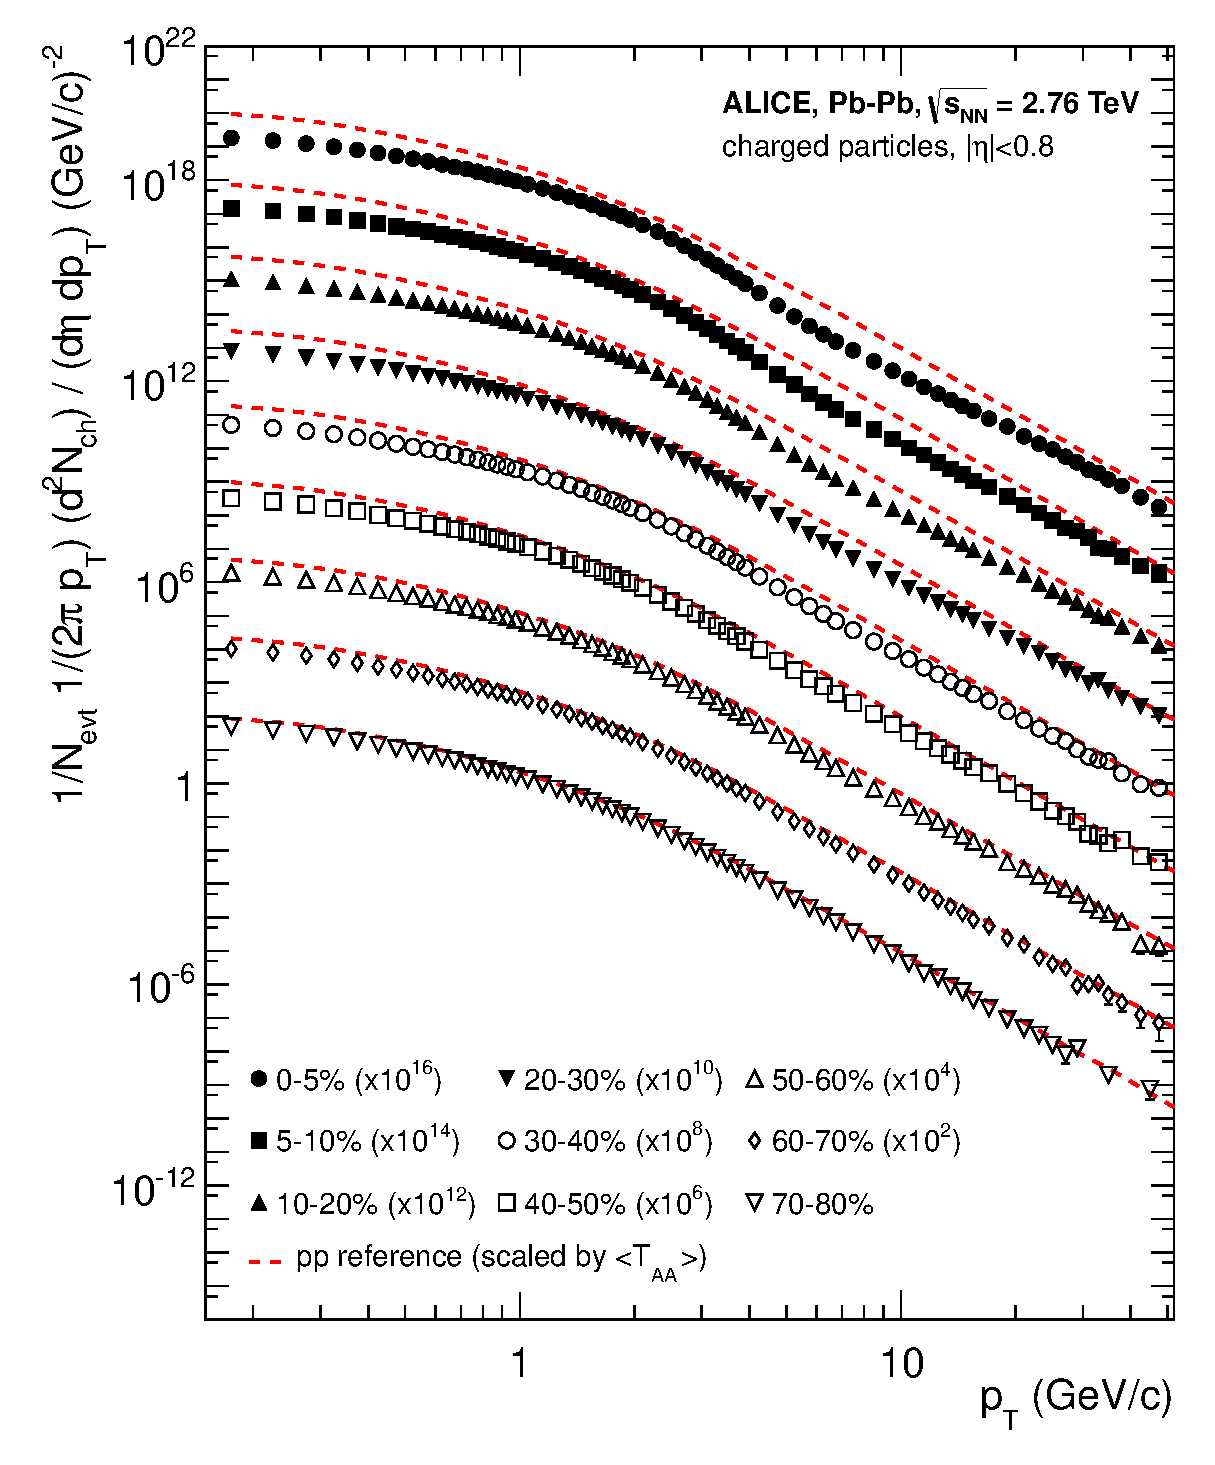
\includegraphics[width=0.6\textwidth]{pics/pT_PbPb}
\caption[Charged particle spectra]{ Charged particle spectra measured by ALICE~\cite{PRL106032301} for the 9 centrality classes given in the legend. The distributions are offset by arbitrary factors given in the legend for clarity. The distributions are offset by arbitrary factors given in the legend for clarity. The dashed lines show the proton-proton reference spectra scaled by the nuclear overlap function determined for each centrality class and by the Pb-Pb spectra scaling factors~\cite{PRL106032301}.}
\label{fig:dndpt}
\end{figure}

The transverse momentum spectra $\dd N/\dd {\pt{}}$ in heavy-ion collisions is shown in Fig. \ref{fig:dndpt}. The vast majority of produced particles have small $\pt{}$. The difference between the yield of $1\gevc$ and $4\gevc$ particles is already 2-3 orders of magnitude. Any observables that are integrated over $\pt{}$ are therefore dominated by the small momentum particles.




\subsubsection{Anisotropic Flow}
In a non-central heavy-ion collision the shape of the impact zone is almond-like. In peripheral collisions the impact parameter is large which means a strongly asymmetric overlap region.  In a central collision the overlap region is almost symmetric in the transverse plane. In this case the impact parameter is small. Collisions with different impact parameters are shown in Fig.~\ref{fig:collisionA}.

\begin{figure}[b!]
\centering
        \begin{subfigure}[b]{0.52\textwidth}
                \centering
            	%\includegraphics[height=2.4in]{pics/InteractionB}
	         \includegraphics[height=2.4in]{figures/tikz/central}

                \caption{Peripheral collision}
                \label{fig:InteractionB}
        \end{subfigure}
        \begin{subfigure}[b]{0.45\textwidth}
                \centering
              % \includegraphics[height=2.4in]{pics/InteractionA}
                \includegraphics[height=2.4in]{figures/tikz/peripheral}

                \caption{Central collision}
                \label{fig:InteractionA}
        \end{subfigure}
	\caption[Illustration of flow in momentum space in central and peripheral collisions.]{Illustration of flow in momentum space in central and peripheral collisions. The density of the arrows represent the magnitude of flow seen at a large distance from the collision in the corresponding azimuthal direction. In a peripheral collision momentum flow into in-plane direction is strong and flow into out-of-plane direction is weak. In a central collision anisotropy in flow is smaller, but the total yield of particles is larger.}
	\label{fig:flow}
\end{figure}

The pressure gradient is largest in-plane, in the direction of the impact parameter $b$, where the distance from high pressure, at the collision center, to low pressure, outside the overlap zone, is smallest. This leads to stronger collective flow into in-plane direction, which in turn results in enhanced thermal emission through a larger effective temperature into this direction, as compared to out-of-plane~\cite{Ollitrault:1992,Ollitrault:1993, Heinz:2002}. The resulting flow is illustrated in Fig.~\ref{fig:flow}. Flow with two maxima in the direction of the reaction plane is called elliptic flow. This is the dominant part of anisotropic flow. Also more complex flow patterns can be identified. The most notable of these is the triangular flow, which is mainly due to fluctuations in the initial conditions.

Flow is nowadays usually quantified in the form of a Fourier composition 

\begin{equation}
E\frac{\dd{^3N}}{\dd {p^3}}=\frac{1}{2\pi}\frac{\dd {^2N}}{\pt{ }\dd {\pt{ }}\dd {\eta} } \left(1+\sum_{n=1}^{\infty}2v_n\left(\pt{},\eta\right)\cos(n(\phi-\Psi_n))\right),
%\label{eq:finalseries}
\end{equation}

\noindent where the coefficients $v_n$ give the relative strengths of different anisotropic flow components and the overall normalisation gives the strength of radial flow. Elliptic flow is represented by $v_2$ and $v_3$ represents triangular flow. The first coefficient, $v_1$, is connected to directed flow. This will however in total be zero because of momentum conservation. It can be nonzero in some rapidity or momentum regions but it must be canceled by other regions.

The first approaches to quantifying the anisotropy of flow did not use the Fourier composition. Instead they approached the problem with a classic event shape analysis using directivity~\cite{danielewicz:1985} or sphericity~\cite{Ollitrault:1992, Danielewicz:1983283} to quantify the flow.


%The first one to predict anisotropic flow in heavy-ion collisions was Ollitrault in 1992~\cite{Ollitrault:1992}. The first papers on anisotropy did not discuss the Fourier composition. Instead they approached the problem with an classic event shape analysis. (sphericity)

The first experimental studies of anisotropy were performed at the AGS~\cite{PhysRevLett.70.1393} in 1993. They noted that the anisotropy of particle production in one region correlates with the reaction plane angle defined in another region. 

The first ones to present the Fourier decomposition were Voloshin and Zhang in 1996~\cite{Voloshin:1994mz}. This new approach was useful for detecting different types of anisotropy in flow, since the different Fourier coefficients give different harmonics in flow. They also show the relative magnitude of each harmonic compared to radial flow.

Some parts of the Fourier composition approach were used for Au-Au collisions at $\snn=11.4\gev$ at AGS in 1994~\cite{Barrette:1994xr}. This analysis still focused on event shapes but they constructed these shapes using Fourier composition from different rapidity windows.


{\color{red} Add a paragraph on the lessions learned from flow studies.}

\FloatBarrier

%\subsubsection{High $\pt{}$ Phenomena}
%The measurement of anisotropic flow coefficients can be extended to very high transverse momenta $\pt{}$. High $\pt{}$ measurements of $v_2$ from CMS~\cite{Chatrchyan:2012xq} are shown in Fig. \ref{fig:highpt}. For high transverse momenta $v_2$ values are positive and they decrease slowly as a function of $\pt{}$. At high transverse momentum the $v_2$ values don't, however, represent flow. 

\FloatBarrier
%\subsubsection{Fluctuations and Event-by-Event Flow}
%The colliding nuclei are not static objects but the distribution of nucleons fluctuates over time. The arrangement of the nucleons at the time of the collision is random, which leads to fluctuations in the initial conditions. The shape of the collision zone is not a perfect almond and it can have a more complex shape. Also the density of the created medium is not homogenous but it can have dense hot spots. The initial density distribution of the created medium is the main reason for anisotropic flow. Because of fluctuations the strength of anisotropic flow is not constant event-by-event.
%
%The existence of more complex density profiles also leads to odd flow harmonics. The basic hydrodynamical approach could only explain elliptic flow and even-harmonics. For a long time it was believed that the odd harmonics would be negligible. In 2007 Mishra {\emph et al.}~\cite{Mishra:2007tw} argued that density inhomogeneities in the initial state would lead to non-zero $v_n$ values for higher harmonics including $v_3$.  It was later noted that higher harmonics of $v_n$ would be suppressed by viscous effects and that the shape of $v_n$ as a function of $n$ would provide another valuable tool for studying $\eta/s$~\cite{Mocsy:2010um}. 
%
%In 2010 significant $v_3$ components were also observed in RHIC data~\cite{Alver:2010gr}. The AMPT model that is also studied in this thesis was able to quantitatively describe the centrality dependence of $v_3$ at RHIC and LHC energies, $\snn=200 \gev$ and $2.76\tev$~\cite{Xu:2011fe}.
%
%%Initial state fluctuations can be modelled using the Glauber model~\cite{Alver:2008zza}. However, so far all models fail to describe the experimental $v_n$ distributions consistently over the whole centrality range~\cite{Jia:2012ve}.
%
%Contrary to elliptic flow higher harmonics are not strongly affected by the centrality of the collision. This supports the theory of higher harmonics being the result of fluctuations. Also $v_2$ measurements of ultra-central collisions give non-zero results for flow, even though the traditional approach based on the anisotropy of the overlap zone gives no prediction of anisotropic flow. This is also the result of fluctuations. Measurement of distributions of $v_n$ coefficients has been performed at ATLAS~\cite{Jia:2012ve}. Their measurements of distributions for $v_2$ in central collisions and for $v_3$ and $v_4$ in general are consistent with a pure Gaussian fluctuation scenario~\cite{Jia:2012ve}.
%
%\begin{figure}[tb]
%	\centering
%	\begin{subfigure}[t]{0.5\textwidth}
%                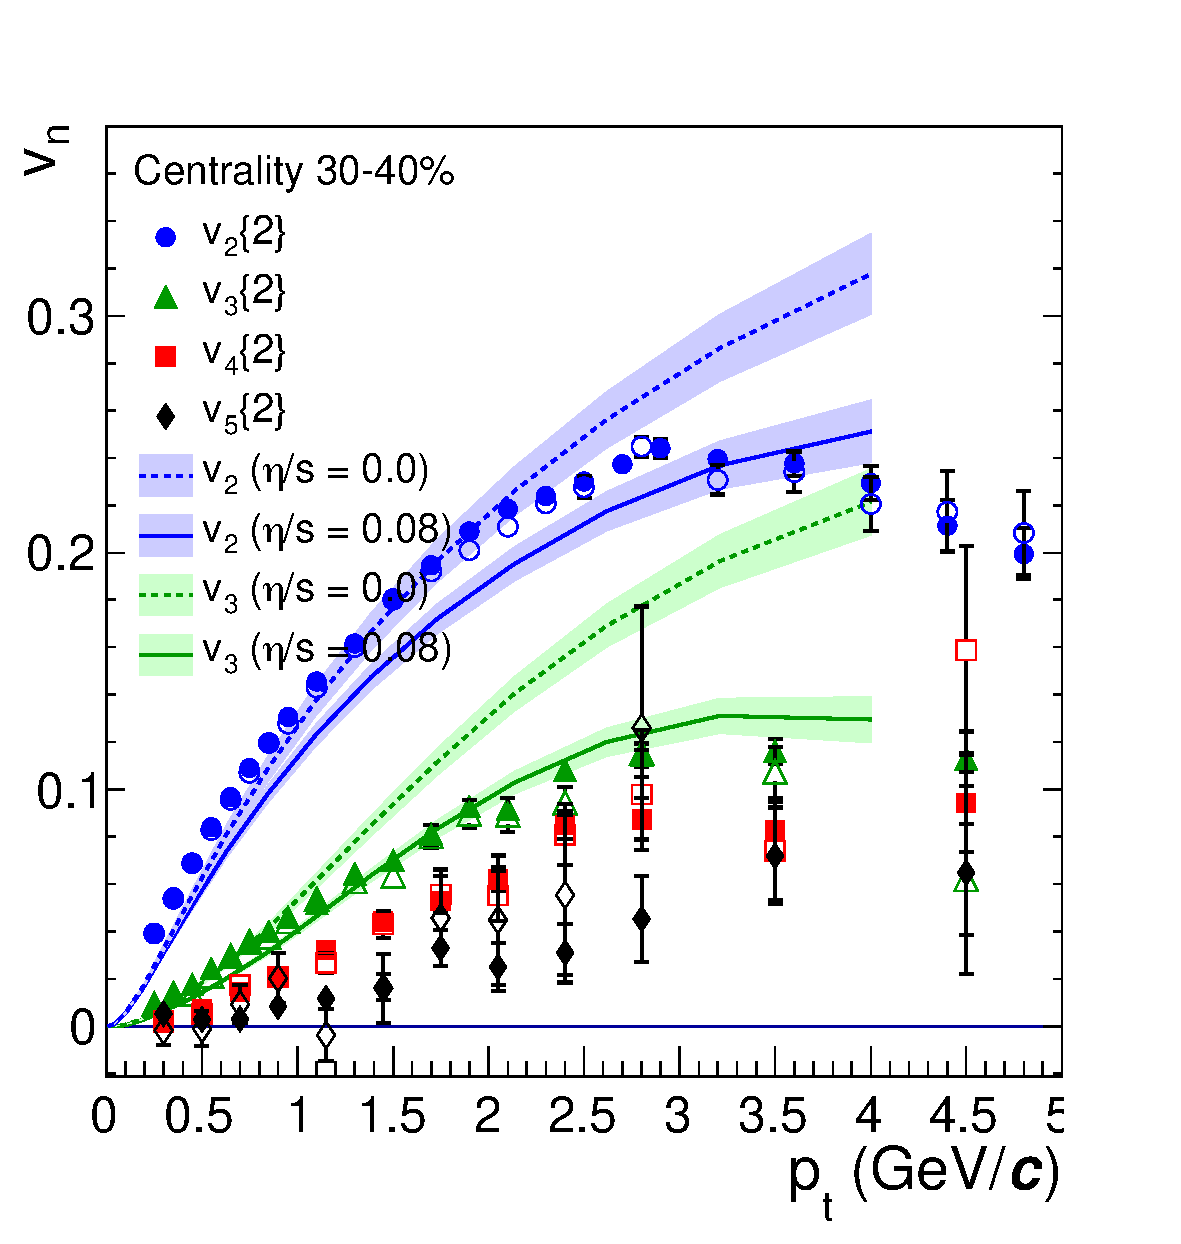
\includegraphics[width=\textwidth]{pics/alice_vn_figa.pdf}
%        \caption[ALICE measurement of $v_2$, $v_3$, $v_4$, $v_5$]{ALICE measurement of $v_2$, $v_3$, $v_4$, $v_5$ as a function of transverse momentum. The flow coefficients are determined by two-particle correlations using different rapidity separations. 
%        The full and open symbols are for $\Delta\eta > 0.2$ and $\Delta\eta > 1.0$. 
%        The results are compared to hydrodynamic predictions~\cite{Schenke:2011tv} with different values of $\eta/s$~\cite{PRL107032301}.}
%        \label{fig:higherharmonics}
%        \end{subfigure}
%        \quad
%        \begin{subfigure}[t]{0.45\textwidth}
%        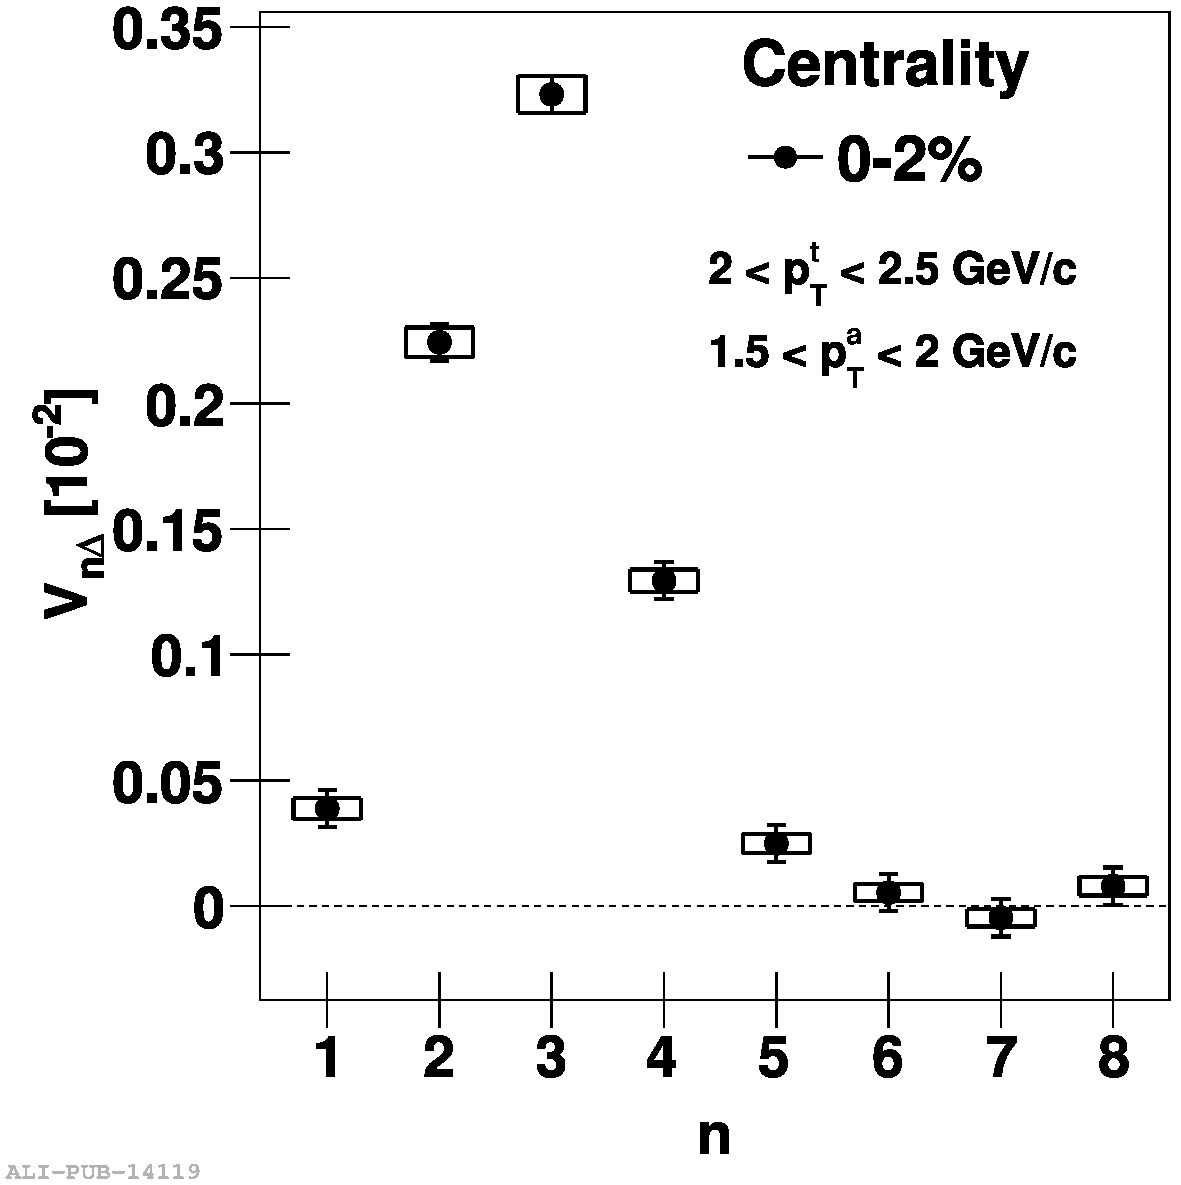
\includegraphics[width=\textwidth]{pics/2012-Jun-06-fig02b}
%        \caption{Amplitude of $v_n$ harmonics as a function of $n$ for the 2\% most central collisions as  measured by ALICE~\cite{Aamodt2012249}.}
%        \label{fig:alicepowers}
%
%        \end{subfigure} 
%        
%%        \begin{subfigure}[t]{\textwidth}
% %               \includegraphics[width=\textwidth]{pics/atlas_powerspectra.png}
%%        \caption{Power spectra of $v_n$ for the 1\% most central collisions measured by ATLAS~\cite{PhysRevC.86.014907}.}
%%        \label{fig:atlaspowers}
% %       \end{subfigure}
%                \caption[Flow measurements of higher harmonics]{Flow measurements of higher harmonics}
%                \label{fig:vnpowers}
%
%\end{figure}
%
%Measurements of different flow harmonics are shown in Fig.~\ref{fig:vnpowers}. The left panel shows different flow harmonics as a function of $\pt{}$ as measured by ALICE~\cite{PRL107032301} in peripheral collisions. In general flow coefficients decrease as a function of $n$ after $n=2$. Central collisions are an exception.The right panel of  Fig.~\ref{fig:vnpowers} shows $v_n$ as a function of $n$ in central collisions as measured by ALICE~\cite{Aamodt2012249}.
%
%
%
%Measurement of event-by-event flow and higher harmonics has growing importance in the field. Triangular flow is useful also for studying jet quenching and in-medium energy loss since anisotropies of flow are related to the path lengths of partons traversing through the medium. Path-lengths and medium density in turn are related the energy loss. An interesting topic of future research would be studying jet properties like $R_{AA}$ separately in events with strong and weak anisotropy.







% !TEX root = thesis.tex

\subsection{Hard processes}
\subsubsection{pQCD factorization}


%\begin{figure}[htb]
%\centering
%\includegraphics[width=0.5\textwidth]{pics/QCDLO}
%\caption[QCD Leading Order]{The basic pQCD processes and their quadratic matrix elements}
%\label{fig:qcdlo2}
%\end{figure}





The term Hard Scattering is used in connection with the scattering of two point-like constituents (partons) of colliding nucleons, when the momentum transfer $Q^2$ is large ($Q \gg \Lambda_{\mathrm{QCD}}$). Figure ~\ref{fig:scattering} shows the incoming partons, quarks or gluons, as they exchange a space-like virtual gluon and produce two highly virtual outgoing partons. The outgoing partons will eventually fragment into collimated showers of partons, referred to as jets.

\begin{figure}[htb]
\centering
\documentclass{standalone}
\usepackage{tikz}
\usepackage{xcolor}
\usetikzlibrary{shapes,arrows}
\usetikzlibrary{trees}
\usetikzlibrary{shadows.blur}
\usetikzlibrary{positioning}
\usetikzlibrary{decorations.pathmorphing}
\usetikzlibrary{decorations.markings}
\begin{document}

\tikzset{
photon/.style={decorate, decoration={snake}, draw=red},
particlearrow/.style={draw=blue, postaction={decorate},
    decoration={markings,mark=at position .5 with {\arrow[draw=black]{>}}}},
antiparticlearrow/.style={draw=blue, postaction={decorate},
    decoration={markings,mark=at position .5 with {\arrow[draw=black]{>}}}},
particle/.style={draw=blue},
antiparticle/.style={draw=blue},
gluon/.style={decorate, draw=orange,
    decoration={coil,amplitude=4pt, segment length=5pt}}
 }
 
 
 
\tikzstyle{proton} = [ellipse, draw=black, text centered, fill=orange!20, minimum height=3em, blur shadow = {shadow blur steps=5},minimum width=1em ] 
\begin{tikzpicture}[node distance=1cm and 1.5cm]
\coordinate[] (p1);
\node[proton, right of=p1]  (proton)  {};
\coordinate[below right=-0.05cm and 0.02cm of proton] (aux1);
\coordinate[above right=-0.05cm and 0.02cm of proton] (aux2);
\coordinate[below right=0.0cm and 2cm of aux1] (vertex1);
\coordinate[right=2cm of aux2] (aux4);
\coordinate[right=2cm of proton] (aux5);
\coordinate[right=2cm of aux4] (spec1);
\coordinate[right=2cm of aux5] (spec2);

\coordinate[below right=1.5cm and 0.5cm of vertex1] (vertex2);

\coordinate[below right=0.0cm and 2cm of vertex2] (b1);
\node[proton, below right=-0.05cm and 0.02cm of b1] (proton2) {};
\coordinate[left=2cm of proton2] (aux6);
\coordinate[below left=-0.05cm and 0.02cm of proton2] (b2);
\coordinate[left=2cm of b2] (aux7);
\coordinate[left=2cm of aux7] (spec3);
\coordinate[left=2cm of aux6] (spec4);
\coordinate[right of=proton2] (p2);
\coordinate[above right=1cm and 1cm of vertex1] (jet1);
\coordinate[below left=1cm and 1cm of vertex2] (jet2);


%Jet cones
\coordinate[above right=1cm and 0.5cm of jet1] (cone11);
\coordinate[above right=0.5cm and 1cm of jet1, label={right:Jet}] (cone12);
\draw[particle] (jet1) -- (cone11);
\draw[particle] (jet1) -- (cone12);
\draw[blue] (cone11) to[out=45,in=45]  (cone12);
\draw[blue] (cone11) to[out=225,in=225] (cone12);

\coordinate[below left=1cm and 0.5cm of jet2] (cone21);
\coordinate[below left=0.5cm and 1cm of jet2, label={left:Jet}] (cone22);
\draw[particle] (jet2) -- (cone21);
\draw[particle] (jet2) -- (cone22);
\draw[blue] (cone21) to[out=45,in=45]  (cone22);
\draw[blue] (cone21) to[out=225,in=225] (cone22);

\draw[particlearrow] (p1) -- node[label=above:$P_A$] {} (proton); 
\draw[particlearrow] (aux1) -- node[label=below:$x_a$] {} (vertex1); 
\draw[particlearrow] (aux2) -- (aux4); 
\draw[particlearrow] (proton) -- (aux5);
\draw[particle] (aux4) -- (spec1);
\draw[particle] (aux5) -- (spec2);
\draw[particle] (aux7) -- (spec3);
\draw[particle] (aux6) -- (spec4);
\draw[particle] (vertex1) -- (jet1);
\draw[particle] (vertex2) -- (jet2);

\draw[gluon] (vertex1) -- node[label=right:$q$] {} (vertex2);
\draw[particlearrow] (b1) -- node[label=above:$x_b$] {} (vertex2);
\draw[particlearrow] (b2) -- (aux7);
\draw[particlearrow] (proton2) -- (aux6);

\draw[particlearrow] (p2) -- node[label=above:$P_B$] {} (proton2);




\end{tikzpicture}



\end{document}

%\includegraphics[width=0.5\textwidth]{pics/ink}
\caption[Hard scattering]{Schematic view of hard scattering process between 2 protons, producing 2 jets}
\label{fig:scattering}
\end{figure}

Historically one would study hard scatterings foremost with inclusive hadron spectra. In this context hadron production from hard scatterings can be factorised into three components; the parton distribution functions $f_a$, $f_b$ that give the probability of getting a parton with momentum fraction $x$ of the proton, the cross section of the elementary scattering $ab\rightarrow cd$,  and the fragmentation functions that give the probability of getting hadron $h$ from the parton.

\begin{equation}
\frac{\mathrm{d} \sigma^h_{pp}}{\mathrm{d}y\mathrm{d}^2\pt{}} = K \Sigma_{abcd}\int \mathrm{d}x_a \mathrm{d}x_b f_a\left(x_a,Q^2\right) f_b\left(x_b, Q^2\right) \frac{\mathrm{d} \sigma}{\mathrm{d}t}\left(ab\rightarrow cd \right)\frac{D_{h/c}^0}{\pi z_c},
\end{equation}

\noindent where 

\begin{equation}
x_{a,b} = \frac{\left| p_{a,b} \right|}{\left| p_{proton} \right|}.
\end{equation}


Parton distribution functions will be discussed further in the following section. The elementary cross section $ab\rightarrow cd$ can be calculated from QCD. A summary of the first order $2\rightarrow2$ processes in QCD is shown in Fig. ~\ref{fig:qcdlo}. 

The final component in the factorization, fragmentation functions, describe the distribution of the fractional momenta of fragments radiated from the outgoing parton.  In a leading order picture, it can be interpreted as the probability that the observed final state originates from a given parton~\cite{Metz:2016swz}. Like the PDFs they are non-perturbative and must be determined experimentally. The measurement is usually performed in $e^+ e^-$ collisions where the kinematics are better controlled. 


%
%\begin{figure}
%\centering
%\includegraphics[width=0.9\textwidth]{pics/Showering}
%\caption[Jet showering]{REPLACE FIGURE An illustration of jet showering. The highly virtual parton from the hard scattering will produce a shower of softer partons. When the virtuality is low enough the shower will go through a hadronisation process that produces the hadrons, which will be eventually observed in the detector. }
%\label{fig:highpt}
%\end{figure}



\begin{figure}[htb]
\centering
\documentclass{standalone}
\usepackage{tikz}
\usepackage{array}
\usetikzlibrary{shapes,arrows}
\usetikzlibrary{trees}
\usetikzlibrary{shadows.blur}
\usetikzlibrary{positioning}
\usetikzlibrary{decorations.pathmorphing}
\usetikzlibrary{decorations.markings}
\begin{document}
\newcommand{\centered}[1]{\begin{tabular}{l} #1 \end{tabular}}

\tikzset{
photon/.style={decorate, decoration={snake}, draw=red},
particlearrow/.style={draw=black, postaction={decorate},
    decoration={markings,mark=at position .5 with {\arrow[draw=black]{>}}}},
antiparticlearrow/.style={draw=black, postaction={decorate},
    decoration={markings,mark=at position .5 with {\arrow[draw=black]{>}}}},
particle/.style={draw=black},
antiparticle/.style={draw=blue},
gluon/.style={decorate, draw=black,
    decoration={coil,amplitude=2pt, segment length=3pt}}
 }
 
%\begin{tabular}{ >{\centering\arraybackslash} m{2cm} >{\centering\arraybackslash} m{2cm} >{\centering\arraybackslash} m{8cm}}
\begin{tabular}{ c c c}

\begin{tabular}{c}
$qq' \rightarrow qq' $ \\
$\bar q q' \rightarrow \bar qq' $
\end{tabular} 
& $\frac{4}{9}\frac{\hat s^2+\hat u^2}{\hat t^2}$

&
\centered{

 \begin{tikzpicture}[node distance=1cm and 1.5cm]
\coordinate[] (e1);
\coordinate[right=1cm of e1] (aux1);
\coordinate[right=1cm of aux1] (e2);
\coordinate[below=1cm of aux1] (aux2);
\coordinate[left=1cm of aux2] (e3);
\coordinate[right=1cm of aux2] (e4);

\draw[particle] (e1) -- (aux1);
\draw[particle] (aux1) -- (e2);
\draw[particle] (e3) -- (aux2);
\draw[particle] (aux2) -- (e4);
\draw[gluon] (aux2) -- node[label=left:$t$] {} (aux1);
\end{tikzpicture} 

}
 \\
$qq \rightarrow qq$ & $\frac{4}{9}\left( \frac{\hat s^2+\hat u^2}{\hat t^2} + \frac{\hat s^2+\hat u^2}{\hat t^2}  \right) - \frac{8}{27}\frac{\hat s^2}{\hat u \hat t}$ &
\centered{

\begin{tikzpicture}[node distance=1cm and 1.5cm]
\coordinate[] (e1);
\coordinate[right=1cm of e1] (aux1);
\coordinate[right=1cm of aux1] (e2);
\coordinate[below=1cm of aux1] (aux2);
\coordinate[left=1cm of aux2] (e3);
\coordinate[right=1cm of aux2] (e4);

\draw[particlearrow] (e1) -- (aux1);
\draw[particlearrow] (aux1) -- (e2);
\draw[particlearrow] (e3) -- (aux2);
\draw[particlearrow] (aux2) -- (e4);
\draw[gluon] (aux2) -- node[label=left:$t$] {} (aux1);
\end{tikzpicture} 

\begin{tikzpicture}[node distance=1cm and 1.5cm]
\coordinate[] (e1);
\coordinate[right=1cm of e1] (aux1);
\coordinate[right=1cm of aux1] (e2);
\coordinate[below=1cm of aux1] (aux2);
\coordinate[left=1cm of aux2] (e3);
\coordinate[right=1cm of aux2] (e4);

\draw[particlearrow] (e1) -- (aux1);
\draw[particle] (aux1) -- (e4);
\draw[particlearrow] (e3) -- (aux2);
\draw[particle] (aux2) -- (e2);
\draw[gluon] (aux2) -- node[label=left:$u$] {} (aux1);
\end{tikzpicture}
}
\\
$\bar q q \rightarrow \bar q' q'$ & $\frac{4}{9}\frac{\hat t^2+\hat u^2}{\hat s^2}$ &
\centered{
\begin{tikzpicture}[node distance=1cm and 1.5cm]
\coordinate[] (e1);
\coordinate[below right=0.7cm of e1] (aux1);
\coordinate[right=1cm of aux1] (aux2);
\coordinate[above right=0.7cm of aux2] (e2);
\coordinate[below left=0.7cm of aux1] (e3);
\coordinate[below right=0.7cm of aux2] (e4);

\draw[antiparticlearrow] (aux1) -- (e1);
\draw[antiparticlearrow] (e2) -- (aux2);
\draw[particlearrow] (e3) -- (aux1);
\draw[particlearrow] (aux2) -- (e4);
\draw[gluon] (aux2) -- node[label=above:$s$] {} (aux1);
\end{tikzpicture}
}
\\
$\bar q q \rightarrow \bar q q$ & $\frac{4}{9}\left( \frac{\hat s^2+\hat u^2}{\hat t^2} + \frac{\hat t^2+\hat u^2}{\hat s^2}  \right) - \frac{8}{27}\frac{\hat u^2}{\hat s \hat t}$ &
\centered{

\begin{tikzpicture}[node distance=1cm and 1.5cm]
\coordinate[] (e1);
\coordinate[below right=0.7cm of e1] (aux1);
\coordinate[right=1cm of aux1] (aux2);
\coordinate[above right=0.7cm of aux2] (e2);
\coordinate[below left=0.7cm of aux1] (e3);
\coordinate[below right=0.7cm of aux2] (e4);

\draw[antiparticlearrow] (aux1) -- (e1);
\draw[antiparticlearrow] (e2) -- (aux2);
\draw[particlearrow] (e3) -- (aux1);
\draw[particlearrow] (aux2) -- (e4);
\draw[gluon] (aux2) -- node[label=above:$s$] {} (aux1);
\end{tikzpicture}
\begin{tikzpicture}[node distance=1cm and 1.5cm]
\coordinate[] (e1);
\coordinate[right=1cm of e1] (aux1);
\coordinate[right=1cm of aux1] (e2);
\coordinate[below=1cm of aux1] (aux2);
\coordinate[left=1cm of aux2] (e3);
\coordinate[right=1cm of aux2] (e4);

\draw[antiparticlearrow] (e2) -- (aux1);
\draw[antiparticlearrow] (aux1) -- (e1);
\draw[particlearrow] (e3) -- (aux2);
\draw[particlearrow] (aux2) -- (e4);
\draw[gluon] (aux2) -- node[label=left:$t$] {} (aux1);
\end{tikzpicture} 
}
\\
$\bar q q \rightarrow gg$ & $\frac{32}{27}\frac{\hat u^2+\hat t^2}{\hat u \hat t} - \frac{8}{3}\frac{\hat u^2 + \hat t^2}{\hat s^2}$ &
\centered{

\begin{tikzpicture}
\coordinate[] (e1);
\coordinate[below right=0.7cm of e1] (aux1);
\coordinate[right=1cm of aux1] (aux2);
\coordinate[above right=0.7cm of aux2] (e2);
\coordinate[below left=0.7cm of aux1] (e3);
\coordinate[below right=0.7cm of aux2] (e4);

\draw[antiparticlearrow] (aux1) -- (e1);
\draw[gluon] (aux2) -- (e2);
\draw[particlearrow] (e3) -- (aux1);
\draw[gluon] (aux2) -- (e4);
\draw[gluon] (aux2) -- node[label=above:$s$] {} (aux1);
\end{tikzpicture}
}
\\
$gg \rightarrow \bar q q$ & $\frac{1}{6}\frac{\hat u^2+\hat t^2}{\hat u \hat t} - \frac{3}{8}\frac{\hat u^2 + \hat t^2}{\hat s^2}$ &
\centered{

\begin{tikzpicture}
\coordinate[] (e1);
\coordinate[below right=0.7cm of e1] (aux1);
\coordinate[right=1cm of aux1] (aux2);
\coordinate[above right=0.7cm of aux2] (e2);
\coordinate[below left=0.7cm of aux1] (e3);
\coordinate[below right=0.7cm of aux2] (e4);

\draw[gluon] (e1) -- (aux1);
\draw[antiparticlearrow] (e2) -- (aux2);
\draw[gluon] (e3) -- (aux1);
\draw[particlearrow] (aux2) -- (e4);
\draw[gluon] (aux2) -- node[label=above:$s$] {} (aux1);
\end{tikzpicture}
}
\\

$q g  \rightarrow qg $ & $\frac{4}{9}\frac{\hat u^2+\hat s^2}{\hat u \hat s} + \frac{\hat u^2 + \hat s^2}{\hat t^2}$ &
\centered{

\begin{tikzpicture}
\coordinate[] (e1);
\coordinate[below right=0.7cm of e1] (aux1);
\coordinate[right=1cm of aux1] (aux2);
\coordinate[above right=0.7cm of aux2] (e2);
\coordinate[below left=0.7cm of aux1] (e3);
\coordinate[below right=0.7cm of aux2] (e4);

\draw[gluon] (e1) -- (aux1);
\draw[gluon] (aux2) -- (e2);
\draw[particlearrow] (e3) -- (aux1);
\draw[particlearrow] (aux2) -- (e4);
\draw[particlearrow] (aux1) -- node[label=above:$s$] {} (aux2);
\end{tikzpicture}

\begin{tikzpicture}
\coordinate[] (e1);
\coordinate[below right=0.7cm of e1] (aux1);
\coordinate[right=1cm of aux1] (aux2);
\coordinate[above right=0.7cm of aux2] (e2);
\coordinate[below left=0.7cm of aux1] (e3);
\coordinate[below right=0.7cm of aux2] (e4);

\draw[gluon] (e1) -- (aux2);
\draw[gluon] (aux1) -- (e2);
\draw[particlearrow] (e3) -- (aux1);
\draw[particlearrow] (aux2) -- (e4);
\draw[particlearrow] (aux1) -- node[label=below:$s$] {} (aux2);
\end{tikzpicture}
\begin{tikzpicture}[node distance=1cm and 1.5cm]
\coordinate[] (e1);
\coordinate[right=1cm of e1] (aux1);
\coordinate[right=1cm of aux1] (e2);
\coordinate[below=1cm of aux1] (aux2);
\coordinate[left=1cm of aux2] (e3);
\coordinate[right=1cm of aux2] (e4);

\draw[gluon] (e1) -- (aux1);
\draw[gluon] (aux1) -- (e2);
\draw[particlearrow] (e3) -- (aux2);
\draw[particlearrow] (aux2) -- (e4);
\draw[gluon] (aux2) -- node[label=left:$t$] {} (aux1);
\end{tikzpicture} 
}
\\
$g g  \rightarrow gg $ & $\frac{9}{2}\left(3- \frac{\hat u \hat t}{\hat s^2}  - \frac{\hat u \hat s}{\hat t^2} -\frac{\hat s \hat t}{\hat u^2}\right)$ &
\centered{
\begin{tikzpicture}[node distance=1cm and 1.5cm]
\coordinate[] (e1);
\coordinate[right=1cm of e1] (aux1);
\coordinate[right=1cm of aux1] (e2);
\coordinate[below=1cm of aux1] (aux2);
\coordinate[left=1cm of aux2] (e3);
\coordinate[right=1cm of aux2] (e4);

\draw[gluon] (e1) -- (aux1);
\draw[gluon] (aux1) -- (e2);
\draw[gluon] (e3) -- (aux2);
\draw[gluon] (aux2) -- (e4);
\draw[gluon] (aux2) -- node[label=left:$t$] {} (aux1);
\end{tikzpicture} 
\begin{tikzpicture}
\coordinate[] (e1);
\coordinate[below right=0.7cm of e1] (aux1);
\coordinate[right=1cm of aux1] (aux2);
\coordinate[above right=0.7cm of aux2] (e2);
\coordinate[below left=0.7cm of aux1] (e3);
\coordinate[below right=0.7cm of aux2] (e4);

\draw[gluon] (e1) -- (aux1);
\draw[gluon] (aux2) -- (e2);
\draw[gluon] (e3) -- (aux1);
\draw[gluon] (aux2) -- (e4);
\draw[gluon] (aux2) -- node[label=above:$s$] {} (aux1);
\end{tikzpicture}

\begin{tikzpicture}[node distance=1cm and 1.5cm]
\coordinate[] (e1);
\coordinate[right=1cm of e1] (aux1);
\coordinate[right=1cm of aux1] (e2);
\coordinate[below=1cm of aux1] (aux2);
\coordinate[left=1cm of aux2] (e3);
\coordinate[right=1cm of aux2] (e4);

\draw[gluon] (e1) -- (aux1);
\draw[gluon] (aux1) -- (e4);
\draw[gluon] (e3) -- (aux2);
\draw[gluon] (aux2) -- (e2);
\draw[gluon] (aux2) -- node[label=left:$u$] {} (aux1);
\end{tikzpicture}

\begin{tikzpicture}
\coordinate[] (e1);
\coordinate[below right=0.7cm of e1] (aux1);
\coordinate[above right=0.7cm of aux1] (e2);
\coordinate[below left=0.7cm of aux1] (e3);
\coordinate[below right=0.7cm of aux1] (e4);

\draw[gluon] (e1) -- (aux1);
\draw[gluon] (aux1) -- (e2);
\draw[gluon] (e3) -- (aux1);
\draw[gluon] (aux1) -- (e4);
\end{tikzpicture}
}


\end{tabular}
\end{document}
\caption[QCD Leading Order]{The basic pQCD processes and their quadratic matrix elements}
\label{fig:qcdlo}
\end{figure}



\subsubsection*{Parton Distribution Function}
Parton Distribution Functions (PDFs) $f_a\left(x\right)$ give the differential probability for parton $a$ to carry momentum fraction $x$ of the proton momentum. %PDFs  are extracted from comprehensive global analysis of experimental results from a variety of fixed-target and collider experiments.
As the PDFs cannot be calculated from first principles they are measured in Deeply Inelastic Scattering (DIS) experiments~\cite{missing} and are extrapolated to the relevant momentum scales using the Dokshitzer-Gribov-Lipatov-Altarelli-Parisi (DGLAP) evolution scheme ~\cite{Gribov:1972ri,Altarelli:1977zs,Dokshitzer:1977sg}  %~\ref{eq:dglap}.

\begin{equation}
\mu_\mathrm{F}^2 \frac{\partial f_i\left(x,\mu_{\mathrm{F}}^2 \right)}{\partial \mu_{\mathrm{F}}^2} = \Sigma_j \frac{\alpha_s\left(\mu_{\mathrm{F}}\right)}{2{pi}} \int _x^1 \frac{\mathrm{d}z}{z} P_{ij}(z) f_j\left(\frac{x}{z},\mu_{\mathrm{F}}^2\right),
\label{eq:dglap}
\end{equation}



\noindent where $\mu_{\mathrm{F}}$ is a factorization scale. The splitting functions $P_{ij}$ describe a probability to radiate parton $i$ from parton $j$ as a function of the momentum fraction $z$ carried away by the offspring parton. Different theory interpretation and experimental data gives rise to different PDF's. Thus there are several commonly used PDF sets: CTEQ~\cite{cteq}, HERAPDF~\cite{CooperSarkar:2011aa}, PDF4LHC~\cite{Butterworth:2015oua}, etc. %Depending on the data used 

\subsubsection{Jet showering}
\label{sec:shower}
\begin{figure}
\centering
\documentclass{standalone}
\usepackage{tikz}
\usepackage{xcolor}
\usetikzlibrary{shapes,arrows}
\usetikzlibrary{trees}
\usetikzlibrary{shadows.blur}
\usetikzlibrary{positioning}
\usetikzlibrary{decorations.pathmorphing}
\usetikzlibrary{decorations.markings}
\begin{document}
\tikzset{
photon/.style={decorate, decoration={snake}, draw=red},
particlearrow/.style={draw=blue, line width=0.75pt, postaction={decorate},
    decoration={markings,mark=at position .5 with {\arrow[draw=black]{>}}}},
antiparticlearrow/.style={draw=blue, postaction={decorate},
    decoration={markings,mark=at position .5 with {\arrow[draw=black]{>}}}},
particle/.style={draw=blue, line width=0.75pt},
hadron/.style={draw=blue,line width=2pt,postaction={decorate},
    decoration={markings,mark=at position .9 with {\arrow[draw=blue]{>}}}},
antiparticle/.style={draw=blue},
gluon/.style={decorate, draw=orange, line width=0.75pt,
    decoration={coil,amplitude=4pt, segment length=5pt}}
 }
\begin{tikzpicture}
%\draw[step = 4cm, gray, thin] (-3cm,-3cm) grid(8,4cm);

\node[ellipse,draw=orange,fill=orange!20, minimum height=1cm, blur shadow = {shadow blur steps=5},minimum width=2cm] (hard) {};
\coordinate[above=1cm of hard, label=Hard Scattering] (label);
\coordinate[left=1cm of hard] (p1);
\coordinate[above left=1cm and 1cm of hard] (p2);
\coordinate[right=1cm of hard] (p3);
\coordinate[below right=1cm and 1cm of hard] (p4);

\coordinate[above right=1cm and 1.25cm of p3] (vertex1_1);
\coordinate[below right=1cm and 1.25cm of p3]  (vertex1_2);

\coordinate[above right=0.75cm and 1cm of vertex1_1] (vertex2_1);
\coordinate[below right=0.3cm and 1cm of vertex1_1] (vertex2_2);
\coordinate[above right=0.3cm and 1cm of vertex1_2] (vertex2_3);
\coordinate[below right=0.75cm and 1cm of vertex1_2] (vertex2_4);


\coordinate[above right=0.75cm and 1cm of vertex2_1] (vertex3_1);
\coordinate[below right=0.3cm and 1cm of vertex2_1] (vertex3_2);
\coordinate[above right=0.3cm and 1cm of vertex2_2] (vertex3_3);
\coordinate[below right=0.3cm and 1cm of vertex2_2] (vertex3_4);
\coordinate[above right=0.3cm and 1cm of vertex2_3] (vertex3_5);
\coordinate[below right=0.3cm and 1cm of vertex2_3] (vertex3_6);
\coordinate[above right=0.3cm and 1cm of vertex2_4] (vertex3_7);
\coordinate[below right=0.75cm and 1cm of vertex2_4] (vertex3_8);


\draw[particlearrow] (p1) -- (hard);
\draw[particlearrow] (p2) -- (hard);
\draw[particlearrow] (hard) -- (p3);
\draw[particlearrow] (hard) -- (p4);

\draw[particle] (p3) -- (vertex1_2);
\draw[gluon] (p3) -- (vertex1_1);

\draw[particle] (vertex1_1) -- (vertex2_1);
\draw[gluon] (vertex1_1) -- (vertex2_2);
\draw[gluon] (vertex1_2) -- (vertex2_3);
\draw[gluon] (vertex1_2) -- (vertex2_4);

\draw[gluon] (vertex2_1) -- (vertex3_1);
\draw[particle] (vertex2_1) -- (vertex3_2);
\draw[particle] (vertex2_2) -- (vertex3_3);
\draw[particle] (vertex2_2) -- (vertex3_4);
\draw[gluon] (vertex2_3) -- (vertex3_5);
\draw[gluon] (vertex2_3) -- (vertex3_6);
\draw[particle] (vertex2_4) -- (vertex3_7);
\draw[particle] (vertex2_4) -- (vertex3_8);

\node[rectangle,draw=orange, fill=orange!20, below right=-0.5cm and 0cm of vertex3_1,minimum width=1cm, minimum height=6cm,label={below:Hadronisation},blur shadow = {shadow blur steps=5}] (hadr) {};

\coordinate[right=0cm of hadr] (hadron1);
\coordinate[right=2cm of hadron1] (detector1);

\coordinate[above=1.5cm of hadron1] (hadron2);
\coordinate[above=2.5cm of hadron1] (hadron3);
\coordinate[below=1cm of hadron1] (hadron4);
\coordinate[below=2.5cm of hadron1] (hadron5);
\coordinate[right=2cm of hadron2] (detector2);
\coordinate[right=2cm of hadron3] (detector3);
\coordinate[right=2cm of hadron4] (detector4);
\coordinate[right=2cm of hadron5] (detector5);


\draw[hadron] (hadron1) -- node[label=above:Hadrons] {}(detector1);
\draw[hadron] (hadron2) -- (detector2);
\draw[hadron] (hadron3) -- (detector3);
\draw[hadron] (hadron4) -- (detector4);
\draw[hadron] (hadron5) --  (detector5);


\end{tikzpicture}
\end{document}

\caption[Jet showering]{An illustration of jet showering. The highly virtual parton from the hard scattering will produce a shower of softer partons. When the virtuality is low enough the shower will go through a hadronisation process that produces the hadrons, which will be eventually observed in the detector. }
\label{fig:showering}
\end{figure}

More detailed studies of the hard processes require a formulation of the showering process. The full picture is a complicated $2\rightarrow n$ scattering, but it is typically seen as a series of $1\rightarrow2$ splittings with decreasing virtuality following the initial $2\rightarrow 2$ scattering~\cite{newPythiaShower}.

To first order the cascade is governed by the DGLAP evolution equation~\cite{Gribov:1972ri,Altarelli:1977zs,Dokshitzer:1977sg}

\begin{equation}
\mathrm{d} P_a\left(z,Q^2\right) = \frac{\mathrm{d}Q^2}{Q^2}\frac{\alpha_s}{2\pi} P_{a\rightarrow bc}\left(z\right)dz,
\label{eq:dglap}
\end{equation} 

\noindent which gives the differential probability that parton $a$ (mother) will branch to two partons $b$ and $c$ (daughters), at a virtuality scale $Q^2$. Daughter $b$ takes a fraction $z$ of the parton $a$ energy and daughter $c$ takes energy fraction $1-z$. The splittings kernels $P_{a\rightarrow bc}\left(z\right)$ are 
\nopagebreak
\begin{align}
P_\mathrm{q\rightarrow qg}\left(z\right) &= \frac{4}{3}\frac{1+z^2}{1-z} \\
P_\mathrm{g\rightarrow gg}\left(z\right) &= 3\frac{\left(1-z\left(1-z \right) \right)^2}{z\left(1-z\right)} \\
P_\mathrm{g\rightarrow q \bar q}\left(z\right)& = \frac{n_f}{2}\left( z^2+\left(1-z\right)^2\right),
\end{align}

\noindent where $n_f$ is the kinematically allowed number of quark flavours. There is some freedom in how the evolution variable $Q^2$ is chosen. If $Q^2=f\left(z \right) m^2$ and $f\left(z \right)$ is a positive and a smooth function it holds that

\begin{equation}
\frac{\mathrm{d}Q^2}{Q^2}\mathrm{d}z = \frac{\mathrm{d} m^2}{m^2} \mathrm{d}z. 
\end{equation}

Of the Monte Carlo generators used in this thesis \pythia~uses $m^2$ as the evolution variable~\cite{missing}, while HERWIG uses an energy-weighted emission angle $E^2\left(1-\cos\theta\right) \approx \nicefrac{m^2}{z\left(1-z\right)}$~\cite{missing}.

Formally eq~\ref{eq:dglap} corresponds to the emission of an infinite number of partons. However very soft and collinear gluons need not considered and one can introduce an effective cut-off scale $Q_0$, usually taken to be of the order of \unit[1]{\gev}.

Going further one approach is to introduce time ordering, i.e. to decide which of the emissions occurs first. This is done in the form of a Sudakov form factor~\cite{missing}

\begin{equation}
P_a^{no}\left(Q^2_\mathrm{max},Q^2\right) = \exp \left(- \int_{Q^2}^{Q^2_\mathrm{max}}\int_{z_\mathrm{min}}^{z_\mathrm{max}} \mathrm{d} P_a \left(z',Q'^2\right)\right),
\end{equation} 

\noindent which gives the probability that no emissions occur between the initial maximum scale $Q^2_\mathrm{max}$ and a given $Q^2$ and within limits $z_\mathrm{min} < z < z_\mathrm{max}$. Thus the probability for the first branching to occur at $Q^2=Q^2_a$ is given by 
\begin{equation}
\dd \Delta_a\left(z,Q_a^2,Q_\mathrm{max}^2\right)=\mathrm{d}P_a \left(z,Q^2_a\right) P_a^{no}\left(Q^2_\mathrm{max},Q_a^2\right).
\end{equation}

Partons $b$ and $c$ that were produced will further branch with maximum virtuality scale $Q^2_\mathrm{max}$ given by $Q^2_a$. Similarly their daughters will continue branching until the cutoff scale is reached, thus producing a shower. 

\begin{figure}[h]
\centering
\begin{tikzpicture}
\tikzset{
photon/.style={decorate, decoration={snake}, draw=red},
particlearrow/.style={draw=blue, postaction={decorate},
    decoration={markings,mark=at position .5 with {\arrow[draw=black]{>}}}},
antiparticlearrow/.style={draw=blue, postaction={decorate},
    decoration={markings,mark=at position .5 with {\arrow[draw=black]{>}}}},
particle/.style={draw=blue},
antiparticle/.style={draw=blue},
gluon/.style={decorate, draw=orange,
    decoration={coil,amplitude=4pt, segment length=5pt}}
 }
 
\coordinate[label=left:$a$] (a);
\coordinate[right=2cm of a] (vertex);
\coordinate[above right=0.5cm and 2 cm of vertex,label=right:$b$] (b);
\coordinate[below right=0.5cm and 2 cm of vertex,label=right:$c$] (c);
\draw[particlearrow] (a) -- (vertex);
\draw[particlearrow] (vertex) -- node[label=above:$z$] {} (b);
\draw[particlearrow] (vertex) -- node[label=below:$1-z$] {} (c);
\end{tikzpicture}
\end{figure}




\subsubsection{Soft gluon radiation and angular ordering}

\begin{figure}[tb]
\centering
\begin{tikzpicture}[scale = 2]
\tikzset{
photon/.style={decorate, decoration={snake}, draw=red},
particlearrow/.style={draw=blue, postaction={decorate},
    decoration={markings,mark=at position .5 with {\arrow[draw=black]{>}}}},
antiparticlearrow/.style={draw=blue, postaction={decorate},
    decoration={markings,mark=at position .5 with {\arrow[draw=black]{>}}}},
particle/.style={draw=blue},
antiparticle/.style={draw=blue},
gluon/.style={decorate, draw=orange,
    decoration={coil,amplitude=4pt, segment length=5pt}}
 }
\coordinate[label=left:$g$] (a);
\coordinate[right=2cm of a] (vertex);
\coordinate[above right = 0.25cm and 1cm of vertex] (vertex2);
\coordinate[above right=1cm and 1cm of vertex2] (gluon);
\coordinate[above right=0.5cm and 2 cm of vertex,label=right:$q$] (b);
\coordinate[below right=0.5cm and 2 cm of vertex,label=right:$\bar q$] (c);
\draw[gluon] (a) -- (vertex);
\draw[particlearrow] (vertex) --  (b);
\draw[particlearrow] (vertex) --  (c);
\draw[gluon] (vertex2) -- (gluon);

\coordinate[label=left:$g$,right=3cm of vertex] (g2);
\coordinate[right=2cm of g2] (vertex3);
\coordinate[left = 1cm of vertex3] (vertex4);
\coordinate[above right=2cm and 3cm of vertex4] (gluon2);
\coordinate[above right=0.5cm and 2 cm of vertex3,label=right:$q$] (b2);
\coordinate[below right=0.5cm and 2 cm of vertex3,label=right:$\bar q$] (c2);
\draw[gluon] (g2) -- (vertex3);
\draw[particlearrow] (vertex3) --  (b2);
\draw[particlearrow] (vertex3) --  (c2);
\draw[gluon] (vertex4) -- (gluon2);
\end{tikzpicture}

\caption{Soft gluon production}
\label{fig:soft}
\end{figure}

Let us now consider a case where a gluon splits into two quarks, and one of the created quarks emits a soft gluon as seen in Fig.~\ref{fig:soft}. In the laboratory frame the time it takes for a gluon to be emitted from a quark can be estimated to be~\cite{basicsofpqcd}



\begin{equation}
t_\mathrm{emit} \approx \frac{1}{E_q},
\end{equation}


\noindent where the energy of the quark is given by $E_q$. In the rest frame of the quark its energy is given by its virtuality $M_\mathrm{virt}$ and assuming the quark is massless the Lorentz factor between the rest frame the laboratory frame is 

\begin{equation}
\gamma = \frac{E_q}{M_\mathrm{virt}}.
\end{equation}

\noindent Thus the emission time can be written as

\begin{equation}
t_\mathrm{emit} \approx \frac{E_q}{M_\mathrm{virt}^2}  = \frac{E_q}{\left(k+p\right)^2},
\end{equation}
\noindent where $k$ and $p$ are the four-momenta of the gluon and the quark after the gluon emission. This can be written open in the laboratory frame. Through assuming that the end products are massless and Taylor-expanding the resulting cosine term gives a form that expresses the emission time using the opening angle $\theta_\mathrm{kq}$ between the quark and the gluon


\begin{equation}
t_\mathrm{emit} \approx \frac{1}{k\theta_\mathrm{kq}^2}.
\end{equation}


\noindent The transverse wavelength of the emitted gluon is $\lambda_\perp^{-1}=k_\perp\approx k\theta_\mathrm{kq}$. Thus we get

\begin{equation}
t_\mathrm{emit} \approx \frac{\lambda_\perp}{\theta_\mathrm{kq}}.
\end{equation}

\noindent The secondary gluon can only probe the quark of the earlier splitting if the transverse wavelength is smaller than the transverse separation of the produced $\mathrm{q \bar q}$ pair. The transverse separation is given by

\begin{equation}
r_\perp^{\mathrm{q \bar q}} \approx \theta_\mathrm{q \bar q} t_\mathrm{emit} \approx \lambda_\perp \frac{\theta_\mathrm{q \bar q} }{\theta_\mathrm{k q} }.
\end{equation}

\noindent Thus in order for the emission to probe the individual quark, the opening angle of the $\mathrm{q \bar q}$ splitting, $\theta_\mathrm{q \bar q}$, must be larger than $\theta_\mathrm{k q}$. If the opening angle $\theta_\mathrm{k q}$ is larger, the gluon can't distinguish between the quark and the antiquark, so it probes the state of the system before the splitting, i.e. it can be treated like it was emitted from the primary gluon.  

This leads to the angular ordering of soft gluon radiation. Each successive angle must be smaller than the previous one. The effect can be calculated in all orders ~\cite{missing} and in the DGLAP formalism one can select the evolution variable $Q^2$ in a way that ensures angular ordering~\cite{missing} as is done in the Herwig MC generator. In \pythia~8 this is strictly not included, but the transverse momentum ordered showers are as accurate in describing the soft gluon emissions as the angular ordered showers~\cite{eventGenerators}.

%(The soft gluon behaves as if testing the colour charge of the jet as a whole)= As a results to describe the jet evolution in terms of independent sequential parton splittings one has to include the Angular ordering (AO) condition. This is implemented differently in Monte Carlo generators. In \pythia 8 this is strictly not included, but the transverse momentum ordered showers are as accurate in describing the soft gluon emissions as the angular ordered showers~\cite{eventGenerators}. In Herwig angular ordering is a consequence of the choice of the evolution variable.



\subsubsection{Jet hadronisation}
When the virtuality of the shower is low enough, the shower starts to hadronise. In this regime the parton shower reaches a scale close to $\Lambda_{\mathrm{QCD}}$ and the perturbative description is no longer valid. Thus the hadronisation stage must be described in a non-perturbative manner. In general hadronisation is assumed to be universal, i.e. it shouldn't depend on the collision energy or system. 
The most simple scenario that is used in several theory calculations is the so-called local parton-hadron duality~\cite{Azimov1985}. In the local parton-hadron duality hypothesis it is assumed that there exists a low virtuality scale $Q_0$ in which the hadronisation happens, that is independent of the scale of the primary hard process. At this scale the partons are transformed into hadrons, assuming that the flow of momentum and quantum numbers for the hadrons can be directly obtained from those of partons introducing only small normalising constants. 

The next sections will present more complicated hadronisation models used in Monte Carlo generators, \pythia~and Herwig.

\subsubsection*{Lund string model}

One common implementation in MC generators is the Lund string fragmentation algorithm~\cite{ANDERSSON198331}. The string model is based on the fact that in QCD linear confinement is expected over large distances~\cite{eventGenerators}. This can be modelled by imagining a colour flux tube being stretched between the outgoing partons. The left side of Fig. ~\ref{fig:fluxtube} illustrates this point for a $\mathrm{q \bar q}$-pair. The tube is assumed to have a uniform fixed transverse size of about \unit[1]{fm} along its length, which leads to a linearly rising potential $V\left(r\right) = \kappa r$, where the string constant $\kappa$ describes the amount of energy per unit length. A value of $\kappa \approx \unit[1]{\GeVfm} \approx\unit[0.2]{GeV^2}$ can be obtained from hadron mass spectroscopy~\cite{missing}.

The evolution of string fragmentation is illustrated schematically on the right side of Fig.~\ref{fig:fluxtube}. This figure is drawn in a light cone presentation, so the initial quark and antiquark are going to separate directions at the speed of light. The string between them, illustrated in the figure by the red line, stretches until its potential energy becomes high enough that it can break, forming a new quark-antiquark pair. If the original pair was $\mathrm{q \bar q}$ and the new pair $\mathrm{q'\bar q'}$, now two new pairs $\mathrm{q \bar q'}$ and $\mathrm{q'\bar q}$ have formed. As these particles are also moving away from each other, the strings between them can stretch and break, creating yet more pairs. The process continues until the invariant mass of the system connected by the string becomes small enough and a final state meson is formed. 

\begin{figure}
\centering
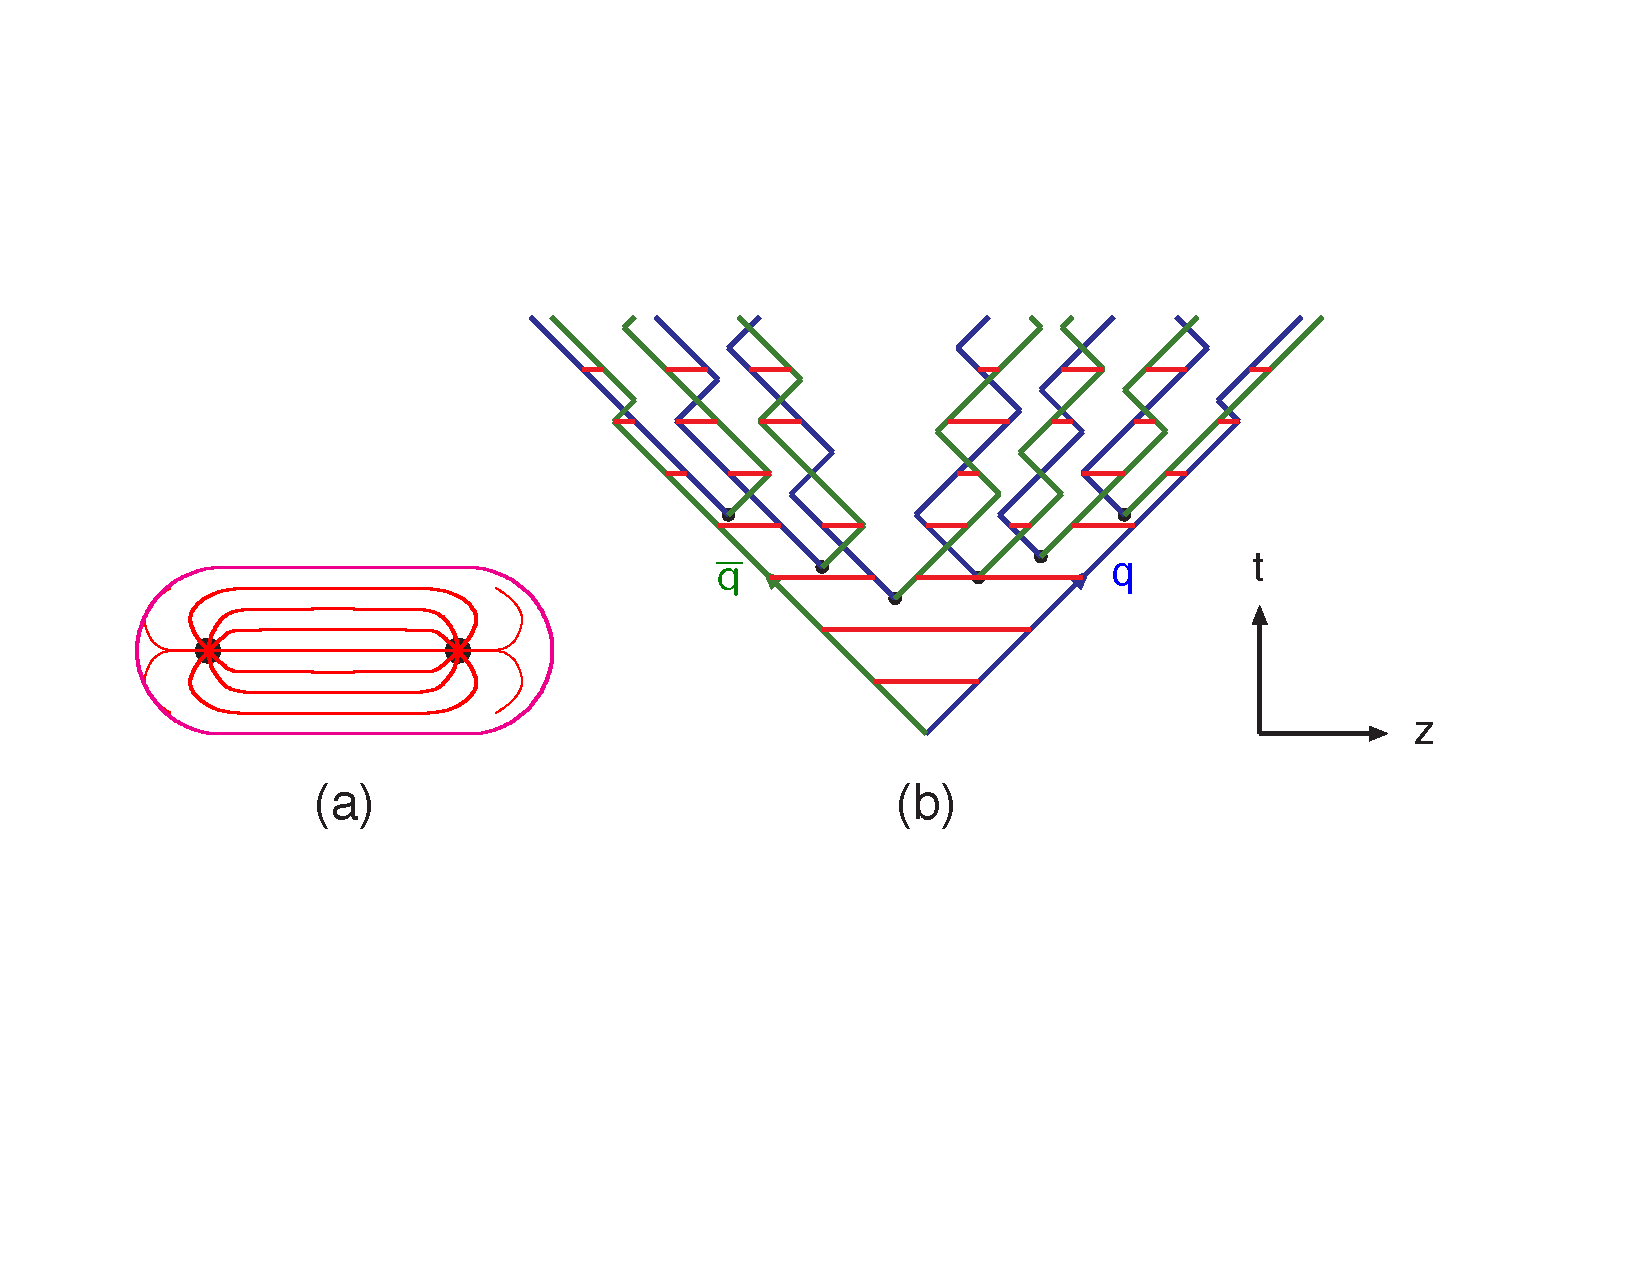
\includegraphics[width=0.75\textwidth]{pics/stringone.pdf}
\caption[]{ (a) A flux tube spanned between a quark and an antiquark. (b) The motion
and breakup of a string system, with the two transverse degrees of freedom suppressed
(diagonal lines are (anti)quarks, horizontal ones snapshots of the string field) \cite{eventGenerators}.
 }
\label{fig:fluxtube}
\end{figure}

To mathematically model the string one can use a massless relativistic string with no transverse degrees of freedom. The gluons are represented as energy and momentum carrying kinks on the string with incoherent sums of one colour charge and one anticolour charge. When this string breaks, it is classically required that the created quark and antiquark are produced at a certain distance if they are to have any mass or transverse momentum. However, taking into account quantum mechanics, the pair must be created at one point and then tunnel out to the classically allowed region. Thus the probability to create a new quark-antiquark pair becomes proportional to the tunnelling probability~\cite{ANDERSSON198331}.


\begin{equation}
P_\mathrm{tunnelling} \propto \exp \left(\frac{-\pi m_\perp^2}{\kappa} \right) = \exp \left(\frac{-\pi m^2}{\kappa} \right) \left(\frac{-\pi p_\perp^2}{\kappa} \right),
\end{equation}

\noindent where the transverse mass $m_\perp$ is defined as $m_\perp^2 = m^2 + p_\perp ^2$. The transverse momentum is now defined to be transverse to the string axis. This formula gives flavour-independent Gaussian $p_\perp$-distribution for the created $\mathrm{q \bar q}$ pairs.

As explained above the string fragmentation would only produce mesons in the final state, but we know that also baryons are created in the process. In the string fragmentation model baryon production is included by adding a probability that a diquark-antidiquark pair is created instead of a quark-antiquark pair when a string breaks.

The kinematics of each string breaking are determined iteratively. Since there is no natural ordering, the string breaking can be considered in any order and the answer obtained must be the same. One can start from the q leg and work one's way to the $\bar{\mathrm{q}}$ leg, or vice versa. This give a left-right symmetry of the string fragmentation. In the Lund model this is taken into account by defining a symmetric fragmentation function

\begin{equation}
f\left(z\right) \propto \frac{1}{z} \left(1-z\right)^a \exp \left(-\frac{b m_\perp ^2}{z} \right)
\label{eq:symmetric}
\end{equation}

\noindent to break the string into a hadron and a remainder system. Here $z$ is the fraction of light-cone momentum $p^+$ given to the hadron in the string breaking, $m_\perp$ is the transverse mass of the hadron and $a$ and $b$ are tuneable parameters of the model. For heavy quarks this is modified as 

\begin{equation}
f\left(z\right) \propto \frac{1}{z^{1+bm_Q^2}} \left(1-z\right)^a \exp \left(-\frac{b m_\perp ^2}{z} \right).
\label{eq:symmetric2}
\end{equation}

\noindent The process can be thought as follows: first start from the q-leg of a $\mathrm{q \bar{q}}$ system and choose to consider the breaking to new $\mathrm{q' \bar q'}$ pair closest to this leg. Now the breaking will produce a hadron $\mathrm{q \bar{q}'}$ and a remainder system spanning from $\mathrm{q' \bar{q}}$. Then the process is continued until the $\bar{\mathrm{q}}$-leg is reached. A small detail here is that in equation (\ref{eq:symmetric}) it is assumed that the mass of the remainder system is large. Thus some patching up is needed for the last two hadrons coming from a string. The patching up is done such that the place where it happens looks as closely like any other string break as possible.


One additional possibility one must consider is that a string can have such a low mass that it cannot break at all. In this case a single hadron is generated out of the string and if necessary  energy and momentum are exchanged with other partons in the event.

After all the hadrons are produced, the short-lived ones can still decay before the set of final state particles in the simulation is obtained~\cite{missing}


\subsubsection*{Cluster model}
Instead of a string model HERWIG~\cite{herwigManual} uses a cluster model for hadronisation. The advantage of cluster models is that they require a smaller number of parameters than string models. The model is based on the preconfinement property of parton showers, i.e. the colour structure of the shower at any evolution scale $Q_0$ is such that colour singlet combinations of partons can be formed with an asymptotically universal invariant mass distribution. The invariant mass does not depend on the initial hard process scale $Q$, but only on $Q_0$ and the QCD scale $\Lambda _ \mathrm{QCD}$, when $Q \gg Q_0$~\cite{missing}.

The cluster model starts from transforming all gluons non-perturbatively into $\mathrm{q \bar q}$ pairs, which requires that the gluons get a mass, which must be at least twice the lightest quark mass. After the gluons are transformed into quarks, the adjacent colour lines can be clustered together to colour singlet states with mesonic quantum numbers. The momentum of these clusters is defined to be the sum of the momenta of the clustering partons. The principle of colour-preconfinement states that the mass distribution of these clusters is independent of the hard scattering process and its centre-of-mass energy~\cite{herwigManual}. %As the mass distribution is peaked at low masses, the clusters can be regarded as highly excited hadron resonances and decayed into the final state hadrons.

Some of these initial clusters are too heavy to reasonably describe an excited state of a hadron. These must be
split before they are allowed to decay. The cluster $C$ is split if its mass fulfils the condition~\cite{herwigManual}

\begin{equation}
M_C^p \geq M_\mathrm{max}^p  + \left( m_1 + m_2\right)^p,
\label{eq:clustermass}
\end{equation}

\noindent where $m_{1,2}$ are the masses of the constituents partons of the cluster. $M_\mathrm{max}$ and $p$ are parameters given defined the model. These have to be chosen separately for clusters containing light, charmed and bottom quarks. When a cluster splits, a pair of light quarks is generated from the vacuum, which form two new clusters, both containing one quark from the original cluster and one from the newly generated pair. The splitting continues until no clusters with masses fulfilling the equation ~\ref{eq:clustermass} remains.

\begin{figure}
\centering
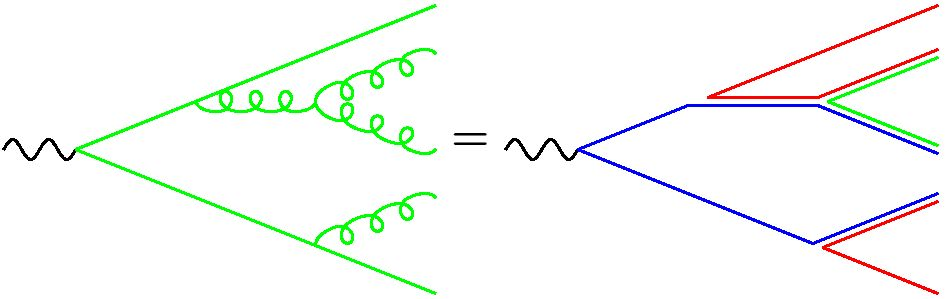
\includegraphics[width=0.75\textwidth]{pics/planar.jpg}
\caption[]{ Colour structure of a parton shower to leading order in Nc.
\cite{eventGenerators} }
\label{fig:colourstructure}
\end{figure}

When the clusters are light enough, they decay into final state hadrons. If the cluster mass is high enough for decaying into a baryon-antibaryon pair, it can undergo either a mesonic or a baryonic decay. The probabilities of mesonic and baryonic decays are parameters in the model~\cite{herwigManual}
%there is a parameter deciding whether the cluster undergoes mesonic or baryonic decay. 
For a mesonic decay a quark-antiquark pair is created from the vacuum and for the baryonic decay a diquark-antidiquark pair is made. Then the exact decay products are chosen and the cluster decays isotropically in the rest frame of the cluster. If there are partons produced in the perturbative phase involved in the decay, they retain their original direction in the cluster rest frame, up to some Gaussian smearing. If the cluster mass is too low to decay into a pair of mesons, it decays into the lightest possible hadron and some energy and momentum is exchanged with the adjacent clusters. At the end we are left with the final state hadrons, some of which might still decay until the end of the simulation if they are very short-lived.~\cite{herwigManual} 

\subsubsection{Interactions between jet and medium}
Let us now look at what happens to jet production in heavy-ion collisions. Figure ~\ref{fig:jetq} shows a dijet produced inside QGP medium. High momentum particles are very rare and they are only produced in the initial collisions. In a heavy ion collision, where a QGP medium is formed, the hard scattered quarks and gluons are expected to interact strongly with the medium due to their colour charges and thus lose energy, either through collisions with medium partons, or through gluon bremsstrahlung~\cite{Connors:2017ptx}. This is referred to as jet quenching.  Studying the modification of jets inside the medium gives another key approach to constraining the properties of QGP. Modification can be also observed in jet shapes, particle composition, fragmentation, splitting functions and many others.


\begin{figure}
\centering
\documentclass{standalone}
\usepackage{tikz}
\usepackage{xcolor}
\usetikzlibrary{shapes,arrows}
\usetikzlibrary{trees}
\usetikzlibrary{shadows.blur}
\usetikzlibrary{positioning}
\usetikzlibrary{decorations.pathmorphing}
\usetikzlibrary{decorations.markings}
\begin{document}

\tikzset{
photon/.style={decorate, decoration={snake}, draw=red},
particlearrow/.style={draw=blue, postaction={decorate},
    decoration={markings,mark=at position .5 with {\arrow[draw=black]{>}}}},
antiparticlearrow/.style={draw=blue, postaction={decorate},
    decoration={markings,mark=at position .5 with {\arrow[draw=black]{>}}}},
particle/.style={draw=blue},
antiparticle/.style={draw=blue},
gluon/.style={decorate, draw=black,
    decoration={coil,amplitude=4pt, segment length=5pt}}
 }
 
 
 
\tikzstyle{proton} = [ellipse, draw=black, text centered, fill=orange!20, minimum height=3cm, blur shadow = {shadow blur steps=5},minimum width=1em ] 
\tikzstyle{protonnoshade} = [ellipse, draw=black, text centered, fill=orange!20, minimum height=3cmminimum width=1em ] 

\begin{tikzpicture}[node distance=1cm and 1.5cm]
\node[proton]  (proton)  {};
\node[proton, right=5cm of proton] (proton2) {};
\coordinate[above right=-0.5cm and 0.03cm of proton] (aux2);
\coordinate[below =0cm of proton] (a);
\coordinate[above=0cm of proton2] (b);
\shade[inner color=red, outer color=yellow] (a) rectangle (b);

\coordinate[right=-0.75cm and 2.5cm of aux2] (vertex1);
\coordinate[left=2cm of proton2] (vertex2);
\node[proton]  (proton3)  {};
\node[proton, right=5cm of proton] (proton4) {};

%\coordinate[below right=1.5cm and 0.5cm of vertex1] (vertex2);

%\coordinate[below right=0.0cm and 2cm of vertex2] (b1);
%\node[proton, below right=-0.05cm and 0.02cm of b1] (proton2) {};
%\coordinate[left=2cm of proton2] (aux6);
%\coordinate[below left=-0.05cm and 0.02cm of proton2] (b2);
%\coordinate[left=2cm of b2] (aux7);
%\coordinate[left=2cm of aux7] (spec3);
%\coordinate[left=2cm of aux6] (spec4);
%\coordinate[right of=proton2] (p2);
\coordinate[above right=1cm and 1cm of vertex1] (jet1);
\coordinate[below left=1cm and 1cm of vertex2] (jet2);


%Jet cones
\coordinate[above right=1cm and 0.5cm of jet1] (cone11);
\coordinate[above right=0.5cm and 1cm of jet1, label={right:Jet}] (cone12);
\draw[particle] (jet1) -- (cone11);
\draw[particle] (jet1) -- (cone12);
\draw[blue] (cone11) to[out=45,in=45]  (cone12);
\draw[blue] (cone11) to[out=225,in=225] (cone12);

\coordinate[below left=1cm and 0.5cm of jet2] (cone21);
\coordinate[below left=0.5cm and 1cm of jet2, label={left:Jet}] (cone22);
\draw[particle] (jet2) -- (cone21);
\draw[particle] (jet2) -- (cone22);
\draw[blue] (cone21) to[out=45,in=45]  (cone22);
\draw[blue] (cone21) to[out=225,in=225] (cone22);

\draw[particlearrow] (aux2) -- node[label=below:$q$] {} (vertex1); 
\draw[particle] (vertex1) -- (jet1);
\draw[particle] (vertex2) -- (jet2);

\draw[gluon] (vertex1) -- (vertex2);
\draw[particlearrow] (proton2) -- node[label=above:$q$] {} (vertex2);

%\draw[particlearrow] (p2) -- node[label=above:$P_B$] {} (proton2);




\end{tikzpicture}



\end{document}

\caption{If hard scatterings happen in conjunction with QGP medium the produced jets must traverse the medium. Thus they are subject to interactions with the medium. Note that the dijet pair can be created anywhere within the medium volume and thus the two jets will have differing path lengths through the medium.}
\label{fig:jetq}
\end{figure}

\subsubsection*{Discovery of jet quenching via leading hadron suppression}
First evidence of jet quenching comes from observing high $\pt{}$ tracks, i.e. the leading hadrons of jets. In this picture jet quenching in heavy-ion collisions is usually quantified with the nuclear modification factor $R_{AA}$, which is  is defined as
%the yield in heavy-ion collisions divided by the yield in proton-proton collisions and scaled by the The nuclear modification factor

\begin{equation}
R_{AA}\left(\pt{}\right) = \frac{(1/N_{AA}^{evt})\dd {N^{AA}}/\dd {\pt{}}}{\left< N_{coll}\right> (1/N_{pp}^{evt})\dd {N^{pp}}/\dd {\pt{}}}\label{eq:raa}
\end{equation}
\noindent where $\dd{N^{AA}}/\dd{\pt{}}$ and $\dd{N^{pp}}/\dd{\pt{}}$ are the yields in heavy-ion and proton-proton collisions, respectively and $\left< N_{coll}\right>$ is the average number of binary nucleon-nucleon collisions in one heavy-ion event. The number of binary collisions can be calculated from the Glauber model as shown in Sec.~\ref{sec:glauber}. From the point of view of direct production at high $\pt{}$ a heavy-ion collision can be estimated relatively well to be only a series of proton-proton collisions. At low $\pt{}$ this scaling breaks down as the determining factor in direct production is the number of participants.


\begin{figure}[hbt]
	\centering
                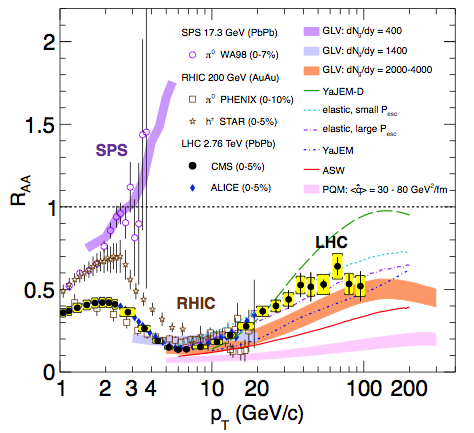
\includegraphics[width=0.65\textwidth]{pics/Raaplot}
        \caption[Measurements of the nuclear modification factor $R_{AA}$ in central heavy-ion collisions]{Measurements of the nuclear modification factor $R_{AA}$ in central heavy-ion collisions at three different center-of-mass energies, as a function of $\pt{}$, for neutral pions ($\pi^0$), charged hadrons ($h\pm$), and charged particles~\cite{Aamodt:2010jd, Aggarwal:2001gn, d'Enterria:2004ig, Adare:2008qa, Adams:2003kv}, compared to several theoretical predictions~\cite{Dainese:2004te, Vitev:2002pf, Vitev:2004bh, Salgado:2003gb, Armesto:2005iq, Renk:2011gj}. The error bars on the points are the statistical uncertainties, and the yellow boxes around the CMS points are the systematic uncertainties. The bands for some of the theoretical calculations represent their uncertainties~\cite{CMS:2012aa}.}
        \label{fig:Raa}
\end{figure}

If the medium has no effect on high $\pt{}$ particles the nuclear modification factor should be 1. As seen in Fig.~\ref{fig:Raa} $R_{AA}$ at RHIC and LHC has been observed to be as low as 0.2, which is a clear signal that jet quenching is happening. However, the physical interpretation is not that 80 \% of high momentum tracks disappear, rather they are shifted to smaller momenta. The relation between the shift in momentum and $R_{AA}$ depends on the steepness of the $\dd{N}/\dd{\pt{}}$ spectra. At LHC energies the spectrum is flatter and thus the same $R_{AA}$ value as in RHIC requires a larger momentum shift, which results from the larger temperature of the medium at LHC. 

The reaction plane dependence of inclusive particle $R_{AA}$ demonstrates that energy loss is path length dependent~\cite{Adler:2006bw}, as expected from models. The path length can be affected by collisions centrality and system size. However, the temperature and lifetime of the QGP also changes with changing centrality and system size. Thus to study different path lengths the angle relative to the reaction plane gives the cleanest signal, as the properties of medium remain the same. Additionally it was concluded that there is no suppression for path lengths below $\mathrm{L} = \unit[2]{fm}$. Similar indications about path length dependence are given by jet $v_2$ both at RHIC~\cite{Adare:2013wop} and at LHC~\cite{Abelev:2012di,Chatrchyan:2012xq}. 



 %Naturally jet quenching depends on the path lengths through the medium.

%\subsubsection*{Theory of jet quenching}


%After the hard partons are created they escape the medium before a thermal equilibrium is reached. Thus they are not part of the pressure-driven collective expansion. Instead high momentum yield is suppressed because of energy loss in the medium. When propagating through the medium these partons lose energy as they pass through the medium. This is referred to as jet quenching. Jet quenching depends on the path lengths through the medium. Thus anisotropy in this region is mainly dependent on the collision geometry and density of medium.


%The energy loss of partons in medium is mainly due to QCD bremsstrahlung and to elastic scatterings between the parton and the medium. 


\subsubsection*{QED Bremsstrahlung}

Many of the energy loss models exploit the analogy between the QCD interaction of parton propagating through the coloured medium and the QED energy loss of electron propagating through material. An electron propagating through matter loses its energy by photon Bremsstrahlung radiation. In the simplest case, each individual scattering center results in a single emission of a photon. This is known as the Bethe-Heitler regime~\cite{BetheHeitler}. The energy spectrum of radiated photons $\nicefrac{\dd N}{\dd E}$ is, in this case, proportional to $\nicefrac{1}{E}$. However, the Bremsstrahlung photon, can be radiated only when the distance between the scattering centers is larger than the formation length. In the limit, when the scattering centers are closer than the formation length, the Bremsstrahlung process is suppressed. This phenomenon is known as the Landau-Pomeranchuk-Migdal (LPM)~\cite{Landau:1953um,Migdal:1956tc} suppression. The radiated spectrum in this regime is proportional to $\nicefrac{1}{\sqrt{E}}$.

Lower energy photons are further suppressed by the destructive interference leading to the suppression of Bremsstrahlung photons of $E < \gamma \omega_p$, where $\omega_p$ is the plasma frequency of the radiator. This is knows as Dielectric suppression. The photon energy distribution in this regime is proportional to the energy of the photon. A schematic view of the effect of these three regimes is shown in Fig.~\ref{fig:bremsstrahlung}.

\begin{figure}[htb]
\centering
\includegraphics[height=2in]{pics/BremsstrahlungElectron}
\caption[Photon spectrum]{ The expected bremsstrahlung spectrum for a electron propagating through material.  ~\cite{Bosted1993QuantummechanicalSO}. }
\label{fig:bremsstrahlung}
\end{figure}

\subsubsection*{QCD}
In QCD the radiative energy loss mechanism is given in terms of the transport coefficient $\left<\hat q\right>$, which describes the average momentum transfer between the medium and parton~\cite{jetBroadeningPpb1}. The exact definition of this depends on the theoretical formalism used to describe the energy loss mechanism. 

The simplest energy loss process is elastic QCD scattering off the medium partons. In elastic scatterings the recoil energy of the scattered partons are absorbed by the thermal medium, which reduces the energy of the initial parton. The mean energy loss from elastic scatterings can be estimated by

\begin{equation}
\left<\Delta E\right>_{\mathrm{el}}=\sigma \rho L \left<E\right>_{\mathrm{1\,scatt}}\propto L,
\label{eq:elastic}
\end{equation}

\noindent where $\sigma$ is the interaction cross section and $\left<E\right>_{1 scatt}$ is the mean energy transfer of one individual scattering~\cite{Majumder:2010qh}. This assumption holds if the mean energy is independent of the total energy of the parton ($E$). The transport coefficient of elastic scattering, $\left< \hat q_\mathrm{el}\right> = \nicefrac{\left< \Delta E\right>}{L}$, is defined as the mean energy los per unit path length.

Another energy loss mechanism is medium-induced radiation. In QCD this radiation is mainly due to the elementary splitting processes, $q\rightarrow qg_r$ and $g\rightarrow gg_r$. Assuming that the parton is moving with the speed of light radiation energy loss can be estimated by

\begin{equation}
\left<\Delta E\right>_{rad}\propto T^3L^2,
\label{eq:radiative}
\end{equation}

\noindent where $L$ is the length of the medium and $T$ is its temperature~\cite{Dominguez:2008vd}. The different exponents of $L$ in equations \ref{eq:elastic} and \ref{eq:radiative} indicate that radiative energy loss is dominant over elastic energy loss.


There are several models that attempt to describe the nature of the energy loss mechanism. The most used models can be divided into four formalisms.
%
%\begin{itemize}
%\item Thermal effective theory formulation (AMY)~\cite{Arnold:2001ms, Arnold:2002ja}
%\item Opacity Expansion ((D)GLV/WHDG and ASW-SH)~\cite{Salgado:2003gb, Gyulassy:2000er, Gyulassy:1999zd, Wiedemann:2000za} 
%\item Higher Twist approach~\cite{Wang:2001ifa, Majumder:2009zu} 
%\item Multiple soft scattering approximation BDMPS-Z (ASW-MS)~\cite{Baier:1996kr, Zakharov:1996fv, Baier:1998kq, Salgado:2003gb}
%\end{itemize}

In the Gyulassy-Levai-Vitev (GLV)~\cite{Gyulassy:1999zd} opacity expansion model
 the radiative energy loss is consiered on a few scattering centers $N_{scatt}$. The radiated gluon is constructed by pQCD calculation as summing up the relevant scattering amplitudes in terms of the number of scatterings. Another approach into opacity expansion is the ASW model by Armesto, Salgado and Wiedermann~\cite{Wiedemann:2000za}.

Thermal effective theory formulation by Arnold, Moore and Yaffe (AMY)~\cite{Arnold:2001ms} uses dynamical scattering centers. It is based on leading order pQCD hard thermal loop effective field theory. This model assumes that because of the high temperature of the plasma the strong coupling constant can be treated as small. The parton propagating through the medium will lose energy from soft scatterings and hard scatterings.

The above models calculate the energy loss while the parton propagates through the medium, focusing on the pQCD part. The higher twist (HT) approach by Wang and Guo~\cite{Wang:2001ifa} implements the energy loss mechanism in the energy scale evolution of the fragmentation functions.

The last category is formed by the Monte Carlo methods. The PYTHIA event generator~\cite{pythia} is widely used in high-energy particle physics. Two Monte Carlo models based on PYTHIA describing the energy loss mechanism are PYQUEN~\cite{Lokhtin:2005px} and Q-Pythia~\cite{Armesto:2009zc}. Other Monte Carlo models include JEWEL~\cite{Zapp:2008gi} and YaJEM~\cite{Renk:2009nz}. 


%\subsubsection*{Discovery of jet quenching via leading hadron suppression}
%First evidence of jet quenching comes from observing high $\pt{}$ tracks, i.e. the leading hadrons.
%Jet quenching in heavy-ion collisions is usually quantified with the nuclear modification factor $R_{AA}$, which is  is defined as
%%the yield in heavy-ion collisions divided by the yield in proton-proton collisions and scaled by the The nuclear modification factor
%
%\begin{equation}
%R_{AA}\left(\pt{}\right) = \frac{(1/N_{AA}^{evt})\dd {N^{AA}}/\dd {\pt{}}}{\left< N_{coll}\right> (1/N_{pp}^{evt})\dd {N^{pp}}/\dd {\pt{}}}\label{eq:raa}
%\end{equation}
%\noindent where $\dd{N^{AA}}/\dd{\pt{}}$ and $\dd{N^{pp}}/\dd{\pt{}}$ are the yields in heavy-ion and proton-proton collisions, respectively and $\left< N_{coll}\right>$ is the average number of binary nucleon-nucleon collisions in one heavy-ion event. The number of binary collisions can be calculated from the Glauber model as shown in Sec.~\ref{sec:glauber}. From the point of view of direct production a heavy-ion collision can be estimated relatively well to be only a series of proton-proton collisions. 
%
%If the medium has no effect on high $\pt{}$ particles the nuclear modification factor should be 1. At RHIC and LHC this has been observed to be as low as 0.2 because of jet quenching. Measurements of $R_{AA}$ from different sources are shown in Fig.~\ref{fig:Raa}
%
%\begin{figure}[hbt]
%	\centering
%                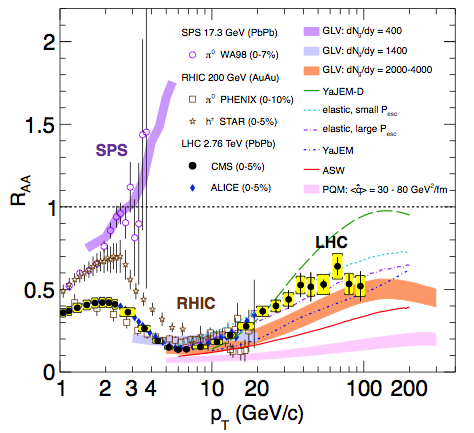
\includegraphics[width=0.65\textwidth]{pics/Raaplot}
%        \caption[Measurements of the nuclear modification factor $R_{AA}$ in central heavy-ion collisions]{Measurements of the nuclear modification factor $R_{AA}$ in central heavy-ion collisions at three different center-of-mass energies, as a function of $\pt{}$, for neutral pions ($\pi^0$), charged hadrons ($h\pm$), and charged particles~\cite{Aamodt:2010jd, Aggarwal:2001gn, d'Enterria:2004ig, Adare:2008qa, Adams:2003kv}, compared to several theoretical predictions~\cite{Dainese:2004te, Vitev:2002pf, Vitev:2004bh, Salgado:2003gb, Armesto:2005iq, Renk:2011gj}. The error bars on the points are the statistical uncertainties, and the yellow boxes around the CMS points are the systematic uncertainties. The bands for some of the theoretical calculations represent their uncertainties~\cite{CMS:2012aa}.}
%        \label{fig:Raa}
%\end{figure}
%
%
%The nuclear modification factor can also be used to quantify anisotropy. In the study of anisotropy $R_{AA}$ in-plane and out-of-plane can be compared, where plane refers to the plane defined by the impact parameter and the beam direction. The distance traveled through medium is largest out-of-plane which leads to stronger suppression in this direction. The nuclear modification factor as a function of $\Delta\phi=\phi-\psi_n$ is given by
%
%\begin{eqnarray}
%R_{AA}\left(\Delta\phi, \pt{}\right) &=& \frac{(1/N_{AA}^{evt})\dd {^2N}^{AA}/d\Delta\phi \dd {\pt{}}}{\left< N_{coll}\right> (1/N_{pp}^{evt})\dd {N^{pp}}/\dd {\pt{}}} \approx \frac{\dd {N^{AA}}/\dd {\pt{}}\left( 1+2\cdot v_2\cos{(2\Delta\phi)} \right)}{\left< N_{coll}\right> \dd {N^{pp}}/\dd {\pt{}}} \nonumber \\ &&\nonumber\\
%&=& R_{AA}^{incl}(\pt{}) \left( 1+2\cdot v_2\cos{(2\Delta\phi)} \right).
%\label{eq:raaandv2}
%\end{eqnarray}	
%
%The yield of proton-proton collisions is independent of the reaction plane and the yield in heavy-ion collisions is modulated by the second harmonics. In Eq. (\ref{eq:raaandv2}) $R_{AA}$ is approximated only up to the second harmonics.
%From \eq{eq:raaandv2} it follows that
%
%\begin{equation}
%\frac{R_{AA}\left(0, \pt{}\right)-R_{AA}\left(\pi/2, \pt{}\right)}{R_{AA}^{incl}(\pt{})} \approx \frac{R_{AA}^{incl}(\pt{}) \left(1+2 \cdot v_2-(1-2 \cdot v_2) \right)}{R_{AA}^{incl}(\pt{})} = 4 \cdot v_2
%\label{eq:raaandv2result}
%\end{equation} 
%%At high-$\pt{}$, the pQCD processes are dominant, hence the $v_n$ (or $R_{AA}(\Delta\phi, \pt{})$) characterize the path length-dependence of the energy loss process. 
%The observed $R_{AA}\left(\Delta\phi, \pt{}\right)$  from PHENIX measurements in Au-Au collisions at $\sqrt{s}=200\gev$~\cite{PhysRevC.80.054907} is compared to $R_{AA}$ using $v_2$  via \eq{eq:raaandv2} in Fig.~\ref{fig:RAAv2}. They agree very well within the statistical errors for all centrality and $\pt{}$ bins.
%\begin{figure}[htb]
%	\centering
%                \includegraphics[width=0.5\textwidth]{pics/RAAandv2Correlation}
%        \caption[A comparison between observed $R_{AA}\left(\Delta\phi, \pt{}\right) $ and $R_{AA}$ using $v_2$]{ A comparison between observed $R_{AA}\left(\Delta\phi, \pt{}\right) $ and $R_{AA}$ using $v_2$ from PHENIX measurements of Au-Au collisions at $\sqrt{s}=200\gev$. On the X-axis is the measured $R_{AA}\left(\Delta\phi,\pt{}\right)$. On the y-axis is the inclusive $R_{AA}$ multiplied by  $1+2v_2\cos\left(\Delta\phi\right)$~\cite{PhysRevC.80.054907}.}
%        \label{fig:RAAv2}
%\end{figure}
%
%At high-$\pt{}$, the pQCD processes are dominant, hence the $v_n$ (or $R_{AA}(\Delta\phi, \pt{})$) characterize the pathlength-dependence of the energy loss process. ~\ref{fig:highpt}
%
%Jet quenching is not the only high $\pt{}$ phenomenon studied in heavy-ion collisions. Another property is jet fragmentation. The high momentum parton created in the initial collision fragments into a number of partons with smaller $\pt{}$. Jet fragmentation occurs also in proton-proton collisions in the vacuum, but it can be modified due to the presence of the medium. In order to study the jet fragmentation function ($D(z)$, where $z= \pt{}^h/\pt{}^{part}$) modification due the medium, we use the two-particle correlations. The particle yield can be extracted from the correlation function. The background from the flow processes is correlated and needs to be subtracted to get the particle yield associated only with the jet. The ratio of the jet yields in Au-Au and p-p collision $I_{AA} = {Y^{Au+Au}}/{Y^{p+p}}$ characterizes the jet fragmentation modification \cite{Aamodt:2011vg}. $I_{AA}$ probes the interplay between the parton production spectrum, the relative importance of quark-quark, gluon-gluon and quark-gluon final states, and energy loss in the medium~\cite{missing}.
%
%
%\begin{figure}[ht]
%\centering
%\includegraphics[width=0.9\textwidth]{pics/fig2_vn_exp-11543.pdf}
%\caption[Elliptic flow, $v_2$ from $\pt{}=1$ to $60\gevc$]{} %Elliptic flow, $v_2$, as a function of the charged particle transverse momentum from $1$ to $60\gevc$ with $\left|\eta\right|<1$ for six centrality ranges in Pb-Pb collisions at $\snn=2.76\tev$, measured by the CMS experiment.~\cite{Chatrchyan:2012xq}. }
%\label{fig:highpt}
%\end{figure}



\subsubsection{New paradigm of jet Quenching}
%As described in the previous section there have been many experimental evidences of jet energy loss, such as the suppression of inclusive hadron spectra at high transverse momentum~\cite{Adcox:2001jp,Adams:2003im,Arsene:2003yk,Khachatryan:2016odn,Acharya:2018qsh}, the modification of back-to-back hadron-hadron~\cite{Adare:2007vu,Aamodt:2011vg} and direct photon-jet correlations~\cite{Adare:2012qi}, and the modification of reconstructed jet spectra~\cite{Adam:2015ewa} and jet substructure~\cite{Sirunyan:2018qec,Chatrchyan:2014ava,Acharya:2018uvf}, as compared to the expectations from elementary proton-proton collisions.


As described in the previous sections the first indications of jet quenching, such as $R_{\mathrm{AA}}$, looked essentially at the leading hadrons of jets, the hard part, ignoring the soft scale part of jet phenomena. However, experimental methods have since improved; jet reconstruction algorithms have become reliable in the LHC era. Instead of the leading hadron we can study the entire jet shower and its structure. In jet observables one must consider what happens to the lost energy. Radiated gluons may end up being clustered with the jet, depending on the radiation angle, the parameters of jet reconstruction and whether the gluon reaches equilibrium with the medium or not. Thus the suppression on the jet level is expected to be smaller. Figure~\ref{fig:jetraa} shows jet $R_{AA}$ in central \PbPb collisions measured by ALICE,ATLAS and CMS and indeed jet $R_{AA}$ is about 0.5 instead of 0.2. %This raises the conceptual question, what counts as being part of the jet.  If a gluon radiated from the jet thermalises with the medium, is it a part of the jet or the medium?


%The first evidence of jet quenching in reconstructed jets at the LHC was observed by measuring the dijet asymmetry, $A_j$ ~\cite{Connors:2017ptx}.  


\begin{figure}
\centering
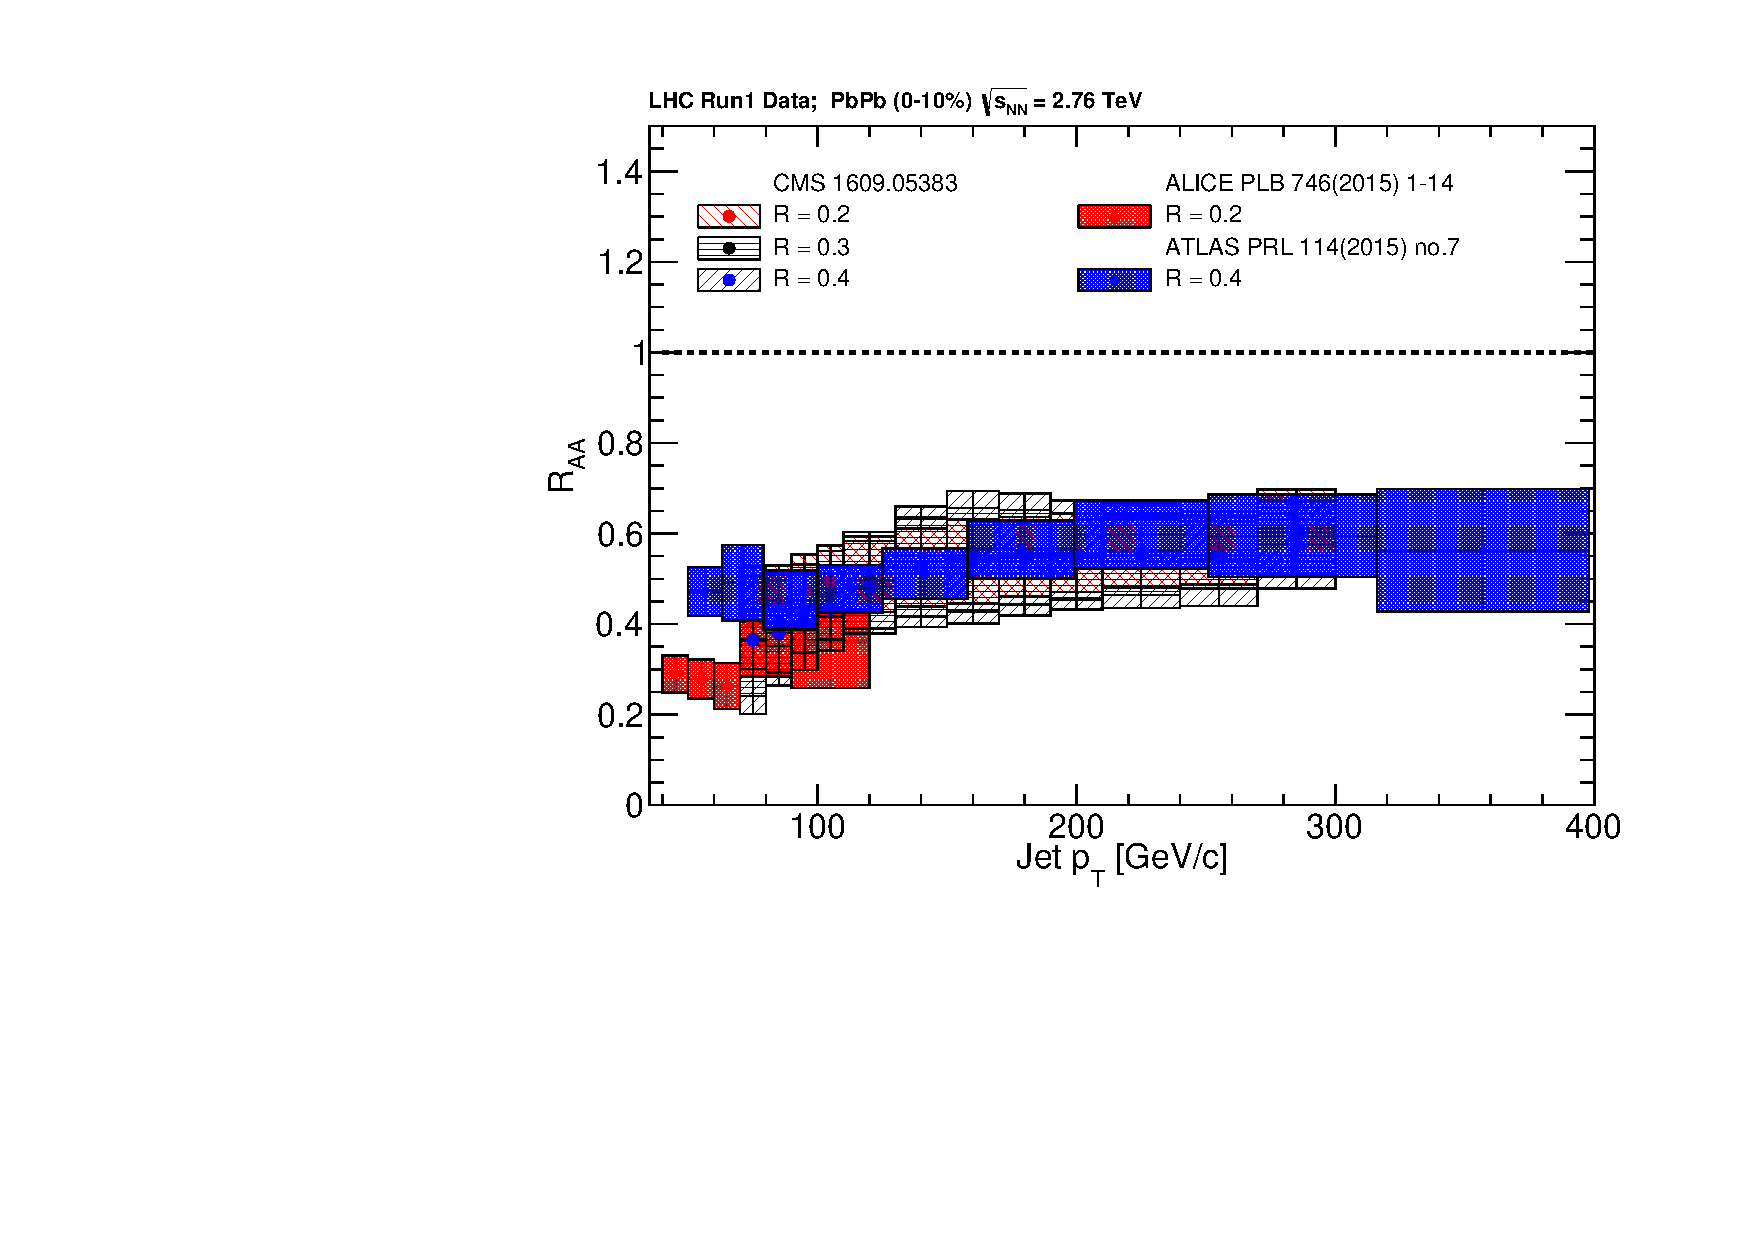
\includegraphics[height=2.4in]{figures/LHC_Run1_RAA_comparison_cent010.pdf}
\caption{Reconstructed anti-$\kt{}$ jet $R_{AA}$ from ALICE~\cite{Adam:2015ewa} with $R = 0.2$ for $\left| \eta \right| < 0.5$, ATLAS~\cite{Aad:2014bxa} with $R = 0.4$ for $\left| \eta \right| < 2.1$, and CMS~\cite{Khachatryan:2016jfl} with R = 0.2, 0.3 and 0.4 for $ \left| \eta \right| < 2.0$. The ALICE and CMS data are consistent within uncertainties while the ATLAS data are higher. The experiments use slightly different methods in selecting jets and subtracting the underlying event contribution. Compared to ALICE and CMS the ATLAS technique could impose a survivor bias and lead to a higher jet RAA at low momenta. Figure from~\cite{Connors:2017ptx}}
\label{fig:jetraa}
\end{figure}

Thus, on the level of the reconstructed jet, energy loss manifests itself as broadening and softening of the jet. This is seen for example in jet-hadron correlations. Figure~\ref{fig:jethadron} shows $\Delta \eta$ correlations with the leading jet. $\Delta \phi$ correlations have similar trends. Jets in \PbPb are observed to be broader, with the greatest increase in the width for low momentum associated particles. This is consistent with expectations from partonic energy loss. These studies found that the subleading jet was broadened even more than the leading jet, indicating a bias towards selecting less modified jets as the leading jet.
Jet hadron correlations have also been studied at RHIC with similar conclusion~\cite{Adamczyk:2013jei}.


\begin{figure}
\centering
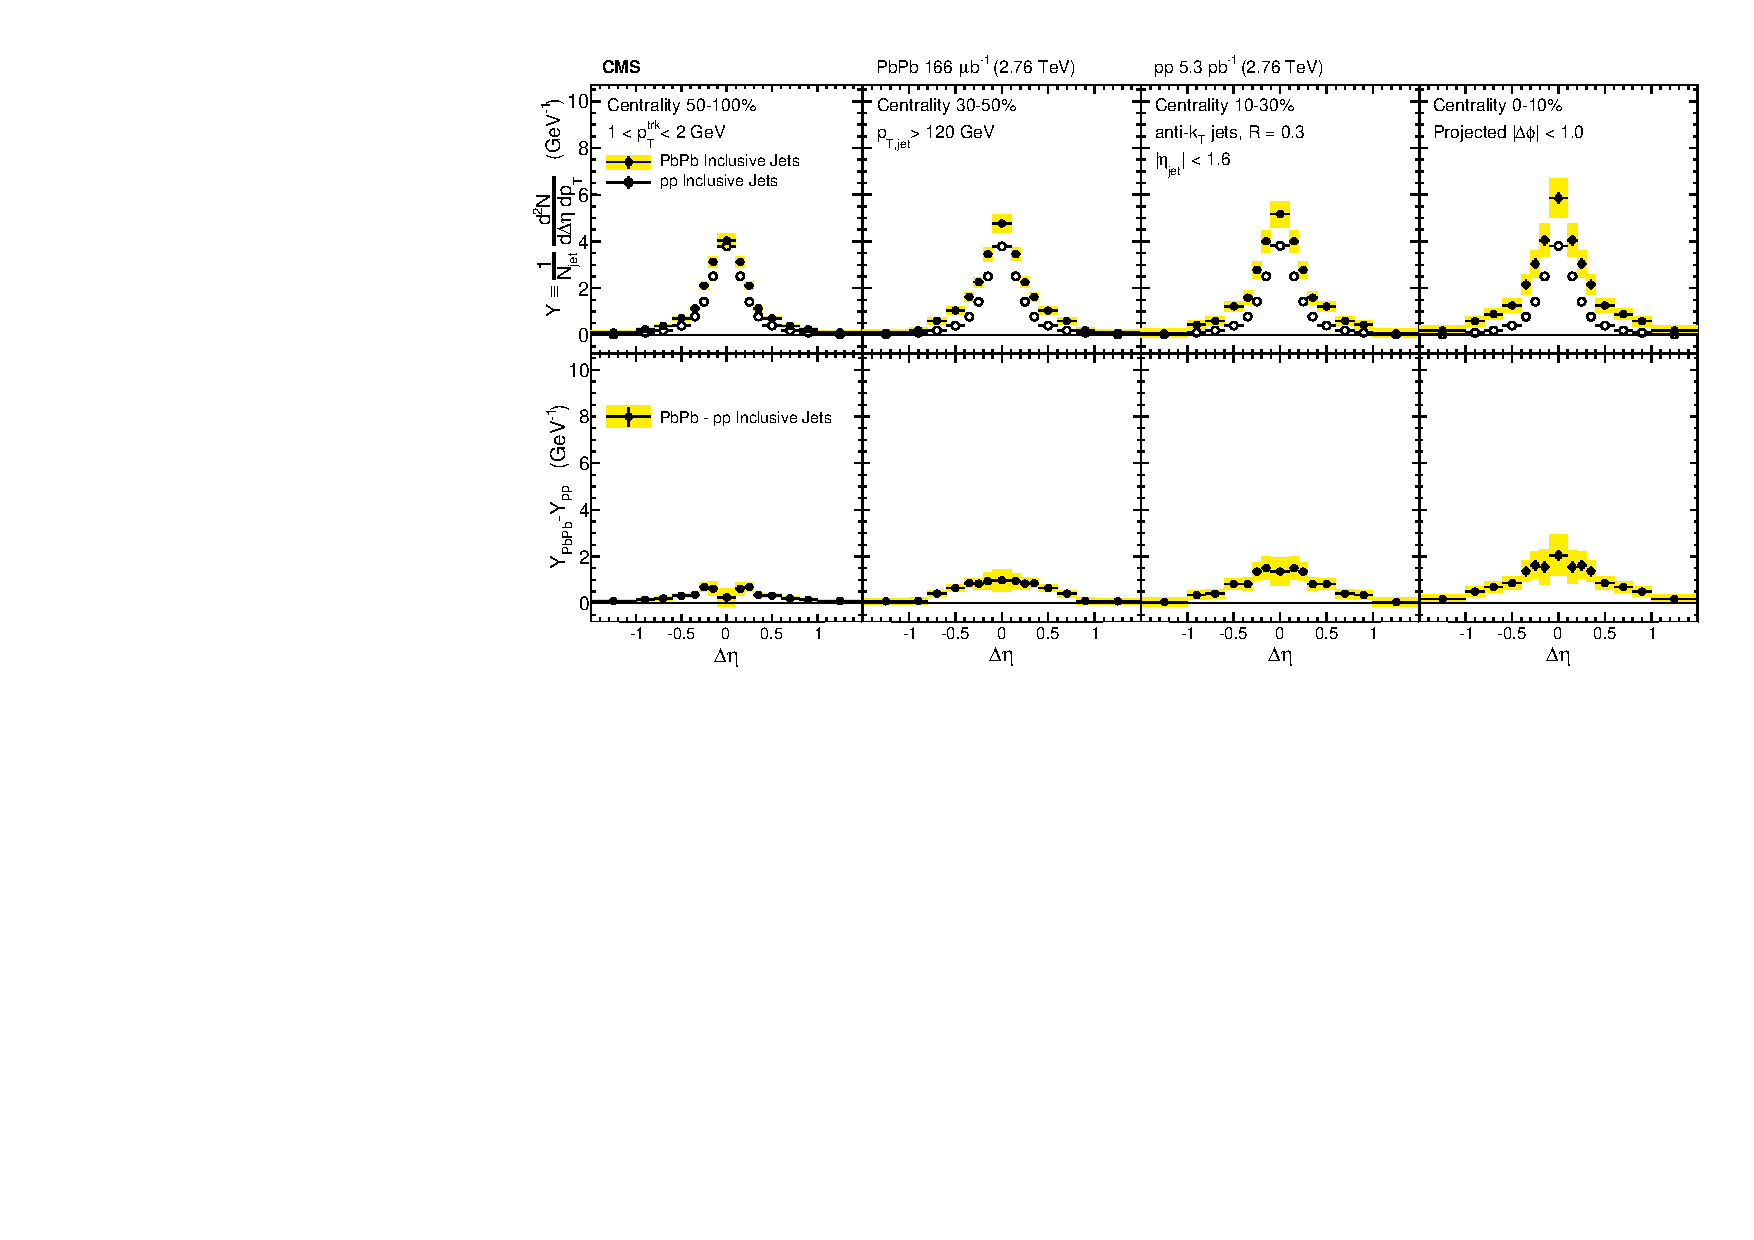
\includegraphics[height=2.4in]{figures/TrackJetCMS-HIN-14-016_Figure_003.pdf}
\caption{Measurement by CMS~\cite{Khachatryan:2016erx}. Symmetrized $\Delta \eta$ distributions correlated with \PbPb and \pp inclusive jets with $\pt{}>\unit[120]{\gev}$ are shown in the top panels for tracks with $1 < \pt{} < \unit[2]{\gev}$. The difference between per-jet yields in \PbPb and \pp collisions is shown in the bottom panels. These measurements indicate that the jet is broadened and softened, as expected. The effect is stronger in more central collisions.  $\Delta \phi$ correlations have similar trends.}
\label{fig:jetraa}
\end{figure}




\subsubsection*{Phase-space view of the medium modified parton cascade}
The new paradigm in jet quenching in heavy-ion collisions involves multi-scale problems~\cite{Kurkela:2014tla,Tachibana:2018yae}. The elementary scattering and the subsequent branching process down to non-perturbative scales are dominated by hard scales in the vacuum as well as in the medium. Soft scales, of the order of the temperature of the medium, characterise the interactions of soft partons produced in the shower with the QGP. Soft scales also rule hadronisation, which is expected to take place in vacuum for sufficiently energetic probes, even though some modifications can persist from modifications of colour flow~\cite{Aurenche:2011rd,Beraudo:2011bh,Beraudo:2012bq}. Understanding the contributions from the different processes to the jet shower evolution in medium and their scale dependence is crucial to to constrain the dynamics of jet energy loss in the expending medium, the role of colour coherence~\cite{CasalderreySolana:2012ef}, and fundamental medium properties like temperature dependent transport coefficient~\cite{DEramo:2012uzl,Ayala:2016pvm}.

\begin{figure}[tbp]
\centering
\begin{subfigure}{0.45\textwidth}
\includegraphics[width=0.99\textwidth]{figures/regions4.eps}
%\caption[]{Illustration of how a medium-modified parton cascade fills the phase space. Early stage vacuum radiation dominates phase space in the DGLAP region. Late stage, after exiting the medium, radiation dominates the Late DGLAP regions.  }
%Parametrically accurate picture of how a medium-modified parton cascade fills the phase space. At time $t$, quanta can be formed up to momentum scale $k_{\rm form}$ and they are formed with $O(1)$ probability per $\log p$ at lower scale $k_{\rm split}$. Quanta below $k_{\rm split}$ split further and their energy cascades to the thermal scale $T$ in less than an epoch $t$. Transverse Brownian motion moves quanta up to the angle $\theta_{\rm BR}(p)$ denoted by the thick purple line.  The Moli\`ere region at larger $\theta$ is dominated by rare large angle scattering. At even larger angle, there are $O(\alpha_s)$ quanta per double logarithmic phase space  from DGLAP 'vacuum' radiation, and for momenta below $k_{\rm split}$ these cascade within time $t$ to $T$. After the jet escapes the medium, the jet and the emitted fragments will undergo vacuum radiation. This late time vacuum radiation emitted by the original parton dominates at sufficiently small $\log \theta$  (regions marked ``late DGLAP'' and bounded by $\theta_{\rm vac}$ and $\theta_\alpha$),  whereas the late time radiation of the fragments dominates in the region  denoted by ``Vacuum cascade of the medium induced quanta''. }
%\label{fig:cascades}
\end{subfigure}
\begin{subfigure}{0.45\textwidth}
\includegraphics[width=0.99\textwidth]{figures/e-vs-th3.eps}
%\caption[]{The distribution of energy as a function of angle for a fixed $p > k_\mathrm{split}$. The  Medium induced radiation dominates around the angular scale $\theta_\mathrm{BR}$. The medium induced contributions (dashed lines) grow as a function of evolution time with respect to the vacuum one (dotted line). ~\cite{Kurkela:2014tla}.}
%\label{fig:edistribution}
\end{subfigure}
\caption{{\it Left}: Phase space view of dominant contributions in a medium-modified parton cascade. {\it Right} The distribution of energy as a function of angle for a fixed momentum with $p > k_\mathrm{split}$. Large angular scales $\theta > \theta_\mathrm{Mol}$ are dominated by DGLAP vacuum radiation from the leading parton at the scale $Q$. At $\theta < \theta_\alpha$ the energy density is dominated by vacuum radiation of the leading parton after it has degraded its energy propagating through the medium. Areas $\theta_\alpha < \theta < \theta_\mathrm{BR}$ and $\theta_\mathrm{BR} < \theta < \theta_\mathrm{Mol}$ are dominated by Brownian motion and rare large angle (Moli\`ere) scatterings with medium partons ~\cite{Kurkela:2014tla}.}
\label{fig:cascades}
\end{figure}

Let us now look at medium modification of jets in a $\log\left(p\right)-\log\left(\theta\right)$ plane as shown in ~\cite{Kurkela:2014tla}. The different momentum and angular scales are subject to different physical phenomena. Figure~\ref{fig:cascades} shows the relevant medium modification phenomena for different regions of the phase space at time $t$, when a jet propagates through a thermal cloud of temperature $T$. As in a practice jets propagate over a finite path-length $L$ in QCD matter, Fig.~\ref{fig:cascades} can be taken as a representation of the distribution of partonic jet fragments at moment $t \approx L$, when the jet escapes the medium.~\cite{Kurkela:2014tla}

The region marked as DGLAP is dominated by the primary vacuum splittings explained in section~\ref{sec:shower}. This region is determined by $\theta > \theta_\mathrm{vac}$ with

\begin{equation}
\theta_\mathrm{vac} \propto \nicefrac{1}{\sqrt{\pt{}}}.
\end{equation}


\noindent Medium-induced parton branching fills the $\log p$-$\log \theta$-plane from the bottom up (in $p$) and from the inside out (in $\theta$). This is because transverse momentum is acquired by Brownian motion in the medium, $k_\perp^2 \propto \hat q t$. The formation time constraint $t \geq \nicefrac{p}{k_\perp^2} \approx \nicefrac{p}{\hat q t}$ implies that medium-induced quanta can be formed in the region $p \leq k_\mathrm{form}$ where

\begin{equation}
k_\mathrm{form}\left(t\right) = \hat q t^2.
\end{equation}

\noindent For these splittees to survive without further splittings they must have 
\begin{equation}
p \geq k_\mathrm{split} \approx \alpha_s^2 k_\mathrm{form}\left(t\right) \approx \alpha_s^2\hat q t^2.
\end{equation} 

\noindent Thus the region marked as LPM in Fig.~\ref{fig:cascades} is filled by the primary medium-induced branchings. Fragments with $p \leq k_\mathrm{split}$ will have time to split further. An approximately equal splitting where both splittees get momentum $~\nicefrac{p}{2}$ from the parent will degrade energy the most. These splittees will undergo the next splitting in an even shorter time scale producing even softer fragments. Momenta can continue cascading all the way to the thermal scale $T$ of the medium within the same time scale within which the first splitting occurred. Thus filling the region marked as Medium cascade in Fig.~\ref{fig:cascade}. Similarly splittees from vacuum radiation can cascade inside the medium when they have $p \leq k_\mathrm{split}$, filling the bottom right corner of the $\log p$-$\log \theta$-plane.

%
%%\begin{equation}
%%\frac{\mathrm d P_\mathrm{find}\left(t\right)}{\mathrm d \log p} \propto \alpha_s \nicefrac{t}{t_\mathrm{form}}\left(p\right) \propto \alpha_s \hat q ^{\nicefrac{1}{2}} p^{-\nicefrac{1}{2}} t
%%\end{equation} 
%
%\noindent Not all quanta will stay where they were created. Those modes that have time to lose a significant fraction of their energy will cascade to a significantly lower scale $p$. For LPM-type radiation, the splitting that degrades energy the most is the hardest splitting. 
%
%The $\log p $ distribution has the same $\frac{1}{\sqrt{p}}$ dependence as in the LPM region
%
%\begin{equation}
%\frac{\mathrm{d}n}{\mathrm{d}\log p} = \frac{1}{p}\frac{\mathrm{d}\epsilon}{\mathrm{d}\log p} \approx \alpha_s \frac{\sqrt{\hat q t}}{\sqrt{p}}
%\end{equation}
%
%\noindent Also the quanta originating from the DGLAP region will undergo medium interactions that will make the quanta radiate and split. The distribution of radiation is the same as from any other mode. Above a certain momentum scale $k_\mathrm{split}$ the distribution of originating daughters is 
%
%
%\begin{equation}
%\frac{\mathrm d P_\mathrm{find}}{\mathrm d \log p \mathrm{d} \log \theta} \approx \alpha_s \frac{t}{t_\mathrm{split}\left(p\right)},
%\end{equation} 
%
%%\noindent Note that the ratio $\nicefrac{t}{t_\mathrm{split}}$ is smaller than 1 for nodes above $k_\mathrm{split}$ and therefore the number of daughters is smaller than the number of vacuum splitted quanta. Below $k_\mathrm{split}$ the cascade is similar to the medium cascade and the number of quanta become
%%
%%\begin{equation}
%%\frac{\mathrm{d}n}{\mathrm{d}\log p \mathrm{d} \log \theta} \approx \alpha_s \frac{t}{t_\mathrm{split}\left(p\right)}, \text{ for } p < k_\mathrm{split}\left(p\right)
%%\end{equation}


The angular distribution of the medium-induced radiation is driven by two mechanisms; Multiple soft scatterings give rise to transverse Brownian motion, which determines the distribution at small angles. The typical angle reached in the LPM region is 

\begin{equation}
\theta_\mathrm{BR}\left(p\right) \approx \frac{\sqrt{\hat q t}}{p}, \text{ for } k_\mathrm{form} > p > k_\mathrm{split},
\end{equation}

\noindent while in the medium cascade region of the phase space this becomes

\begin{equation}
\theta_\mathrm{BR}\left(p\right) \approx \left(\frac{T}{p}\right)^{\frac{3}{4}}
\end{equation}

\noindent Large angular scales cannot be reached by Brownian motion, but can arise from rare large angle scatterings with partons in the medium, described first by Molière~\cite{missing}. The result is that medium-induced radiation is predominantly located in the bands marked as Brownian motion, where $\theta_\alpha < \theta < \theta_\mathrm{BR}$, and Moli\`ere, where $\theta_\mathrm{BR} < \theta < \theta_\mathrm{Mol}$ in Fig.~\ref{fig:cascade}. 

The hard parton will naturally continue radiating after it leaves the medium. As there is no longer kinematic limits set by the time scale, the vacuum radiation can extend to smaller angular scales in the phase space. The results is that the regions, where $\theta<\theta_\alpha$, marked as Late DGLAP in Fig.~\ref{fig:cascade} will be dominated by the late time vacuum radiation. Naturally also the splittees from medium-induced radiation will undergo the late stage vacuum radiation phase, filling the triangular region with small $p$ and $\theta < \theta_\mathrm{\alpha}$.



\subsubsection*{Influence of jet on medium}
Energy loss of hard partons is well established by experimental observations. Naturally energy can't just disappear, but is transferred to daughter partons or the medium. For radiation that stays inside the jet cone energy loss manifests itself as softening and broadening. If a daughter parton loses energy and becomes equilibrated with the medium it may no longer be correlated with the parent parton. This energy would then be distributed at distances far from the jet cone. There is some evidence for out-of-cone radiation by CMS~\cite{Chatrchyan:2011sx}, but the interpretation is not clear. Other possible phenomena include the mach cone and Moliére scattering, but there is no experimental evidence for these. Evidence for all of these effects is difficult to find as the underlying event gives already a large and fluctuating background. Additionally its unclear how this energy would be different from the underlying event~\cite{Connors:2017ptx}.

% !TEX root = thesis.tex

\subsection{QGP in Small systems}
\label{sec:smallsystem}
After the existence of QGP in heavy-ion collisions has been established, attention has been turned to small systems. Proton-proton (\pp) and proton-Lead (\pPb) collisions have been studied at LHC and RHIC has studied a host of different collision systems; namely proton-gold (pAu)~\cite{Aidala:2016vgl}, deuteron-gold (dAu)~\cite{Adler:2003ii,Arsene:2003yk,Back:2003ns,Adams:2003im} and helium$^3$-gold (He$^3$Au)~\cite{Adare:2015ctn} collisions starting from 2000. %At LHC small systems have been studied in proton-Lead (pPb) collisions. First observations seemed to indicate that the signals taken to confirm the existence of QGP in heavy-ion collisions disappear in these small systems.

Already before the era of modern colliders, collective behaviour in proton-proton collisions was considered by names like Heisenberg, Fermi and Bjorken~\cite{Nagle:2018nvi}. Eventually there were some experimental searches of QGP in pp and $p\bar p$ collisions in E735 at Tevatron~\cite{Alexopoulos:1993wt} and MiniMAX~\cite{Brooks:1999xy}. However no conclusive evidence was found. 

In the early years of RHIC these small systems were mostly considered as control measurement, for example in constraining nuclear modified parton distribution functions (nPDFs) that determine the initial gluon distributions that determine the first epoch of heavy-ion collisions~\cite{Shen:2015qta, Adare:2015lcd}. 

In 2010 ultrahigh-multiplicity pp collisions were studied at CMS~\cite{Khachatryan:2010gv}. The study found that particles had a weak but clear preference to be emitted along a common transverse $\phi$ angle across all rapidities ~\cite{Salgado:2016jws}. This seemed like behaviour were similar to AA collisions, but it was argued that it could as well come from momentum correlations present in the earliest moments of the collision.

In 2012 LHC ran its first \pPb data taking period. Around the same time dAu data was re-examined at RHIC. Now it was revealed that most of the flow signatures attributed to hydrodynamic expansion in AA collisions also existed in smaller systems.



%-Sub nucleonic structure needed to describe intial conditions in pA, pp
%\FloatBarrier

\subsubsection{Collective phenomena}
The most rugged analysis of collective behaviour concerns the two (or more) particle correlations, often parametrised via the relative azimuthal angle and pseudorapidity differences, $\Delta \phi$ and $\Delta \eta$ respectively. Figure~\ref{fig:smallsystems2} shows two-particle correlations measurements in \PbPb, \pPb and \pp collisions at the LHC~\cite{Aad:2015gqa}. In \PbPb collisions long-range correlations dominate over short-range phenomena. This shows in the two ridges at $\Delta \phi = 0 $ and $\Delta \phi = \pi$. At $\Delta\phi\approx\Delta\eta\approx0$, there is a peak coming from single jet fragmentation. Since the away-side jet can be spread out in $\Delta\eta$, this contribution disappears when compared to the flow contribution at the away side ridge. In pPb, and pp the near side peak is more distinguished and the away-side jet contribution starts to show. Still, one can see long-range correlations that seem like flow-like collective behaviour in both systems. 
\begin{figure}[b!]
\centering
            	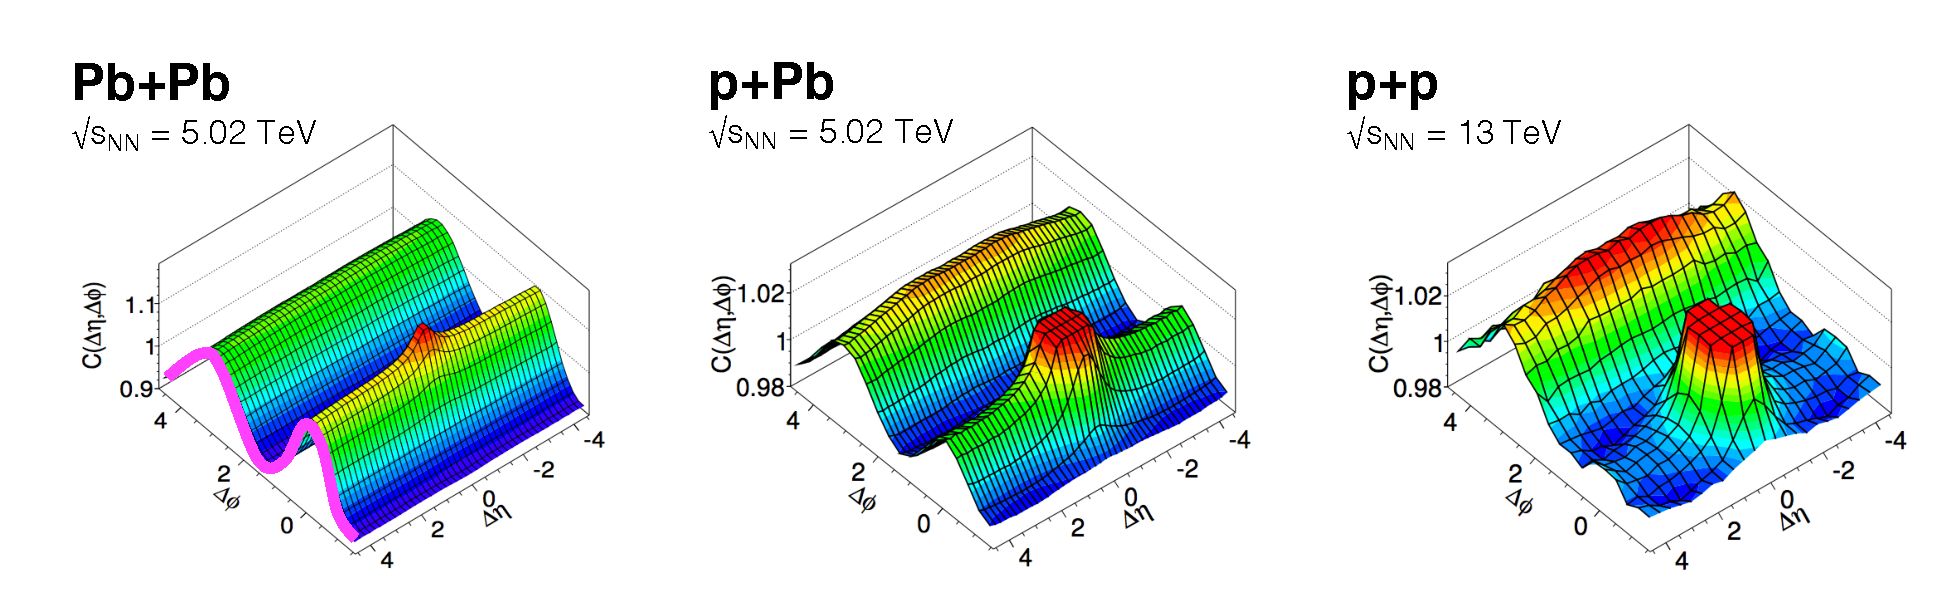
\includegraphics[width=0.9\textwidth]{pics/figure_ridges}
                \caption{Two-particle correlation results in PbPb, pPb, and pp collisions at the LHC~\cite{Aad:2015gqa}. }
	\label{fig:smallsystems2}
\end{figure}

In addition to the two particle correlations, correlations have been observed in the form of $v_n$ coefficients both at LHC~\cite{Acharya:2017ino} and at RHIC~\cite{Aidala:2016vgl}. The results have also been described  with hydrodynamical models, although the applicability of said models might be questionable, because of the large Reynolds numbers in small systems~\cite{Shen:2016zpp,Niemi:2014wta}. Figure~\ref{fig:smallsystems1} shows results for $v_2$ in different collisions systems at RHIC as measured by PHENIX and Figure~\ref{fig:smallhydro} shows the eccentricities and the resulting hydrodynamic evolution in the systems. These different systems provide also different initial geometries. dAu collisions naturally have an ellipsoidal form, while a $\mathrm{He}^3$ collision has a triangular form and thus produces larger triangular flow, $v_3$ components. 

\begin{figure}[htb]
\centering

		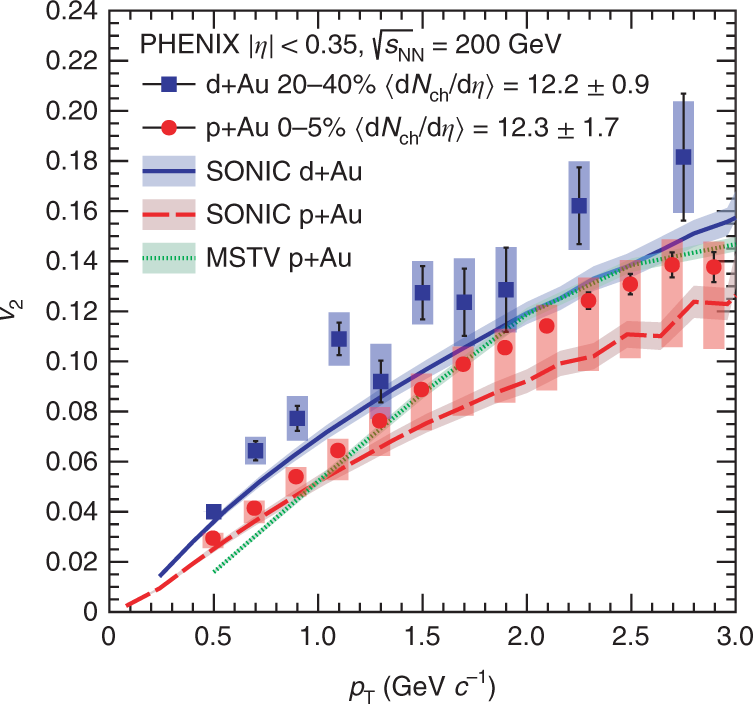
\includegraphics[width=0.5\textwidth]{figures/41567_2018_360_Fig4_HTML.png}
                \caption{Comparison between hydrodynamic calculations and data from $p+\mathrm{Au}$, $d+\mathrm{Au}$ and $^3\mathrm{He+Au}$ collisions~\cite{PHENIX:2018lia}}
	\label{fig:smallsystems1}
\end{figure}

\begin{figure}[b!]
\centering
            	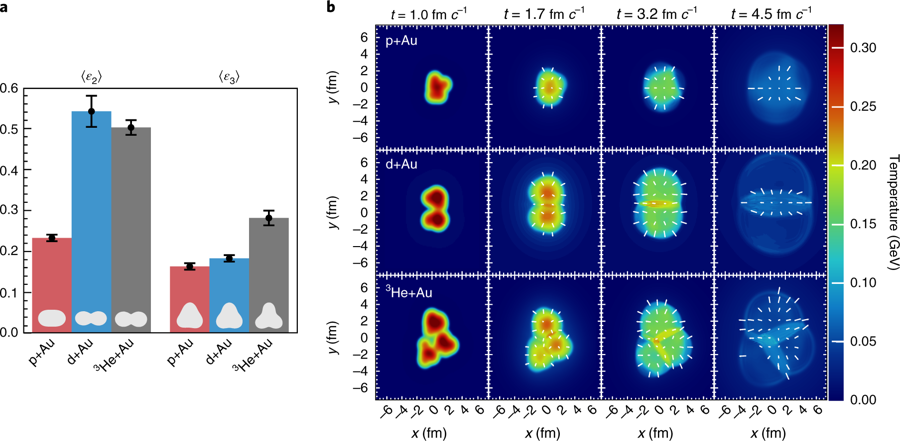
\includegraphics[width=\textwidth]{figures/PhenixNature_1.png}
	\caption{{\it left} Eccentricities in different systems. {\it right} Calculations of the initial energy density in small collision systems at RHIC and the resulting hydrodynamic evolution~\cite{PHENIX:2018lia}.}
	\label{fig:smallhydro}
	\end{figure}


%Citation to ALICE result for mass ordered v2
Other observations that produce flow-like results include mass ordered $v_2$ coefficients~\cite{CMS:2018rfr} and higher order harmonics coming from fluctuations in the initial geometry~\cite{Acharya:2017ino}. Thus all the major collective flow phenomena observed in heavy-ion collisions have been also identified in small systems.

One open question is identifying the point the point, where flow-like correlations end. The question has proved challenging since low multiplicity events are dominated by non-flow phenomena. This makes observations in low multiplicity events model/method dependant. Different methods assess non-flow contributions differently. Thus some methods fail to observe a signal in cases, where others do and it is unclear whether this is true collective motion or it comes from non-flow contributions.

%\FloatBarrier

\subsubsection{Absence of jet quenching}
In A+A collisions, an important confirmation of the standard model comes from the energy loss of high $\pt{}$ partons traversing the medium, as discussed in Section~\ref{sec:energyloss}.
%referred to as jet quenching~\cite{Gyulassy:2003mc,doi:10.1146,Accardi:2009qv}.
Originally the interest in small systems was due to ruling out possible cold nuclear matter effects that might affect the results also in $\PbPb$. In 2003 the jet quenching effect was observed to disappear in d+Au collisions at RHIC~\cite{Adler:2003ii,Adams:2003im,Arsene:2003yk,Back:2003ns}. This was taken as an indication that no QGP was created. Similarly at LHC no jet modification has been observed in pPb collisions. Figure~\ref{fig:smallsystems3} shows the nuclear modification factor $R_{\mathrm{pA}}$ and $v_2$ in pPb collisions as measured at the LHC~\cite{Khachatryan:2016odn,Aad:2014lta}. 

Now the lack of jet modification seems surprising considering the multitude of flow observations supporting the existence of QGP in small systems. One possible explanation is simply the size of medium. In PbPb collision partons traversing through the medium lose energy to the medium. If the medium is very small there is limited time for interaction with the medium. Reaction plane dependent $R_{AA}$ measurements~\cite{Adler:2006bw} in \PbPb collisions indicated that \unit[2]{fm} could be the minimum path length required for energy loss.

Some calculations~\cite{Zhang:2013oca,Park:2016jap,Tywoniuk:2014hta} indicate that there should be modification in the most central \pPb collisions, but selecting these in the analysis is complicated~\cite{Nagle:2018nvi}. In \PbPb collisions most of the particle production comes from the medium and thus the total multiplicity is a good indicator of centrality. However in \pPb collisions the total multiplicity is smaller and is more strongly influenced by jet phenomena. Events with jets have naturally larger multiplicities and are more likely to be classified as central events.

So far the only observable indicative of jet quenching in pPb collisions is the high $\pt{}$ $v_2$. In heavy-ion collisions this is not explained by hydrodynamics. Instead it is assumed to come from jet quenching with different path lengths through the medium in different directions. In Figure~\ref{fig:smallsystems3} ATLAS~\cite{Aad:2014lta} and CMS~\cite{Sirunyan:2017pan} measurements of $v_2$ in pPb and PbPb collisions are shown. The pPb results seem to follow a very similar pattern. However, the non-flow effects in this high-\pt{} region are not fully under control, so the physical interpretation is still under debate. 


\begin{figure}[b!]
\centering
            	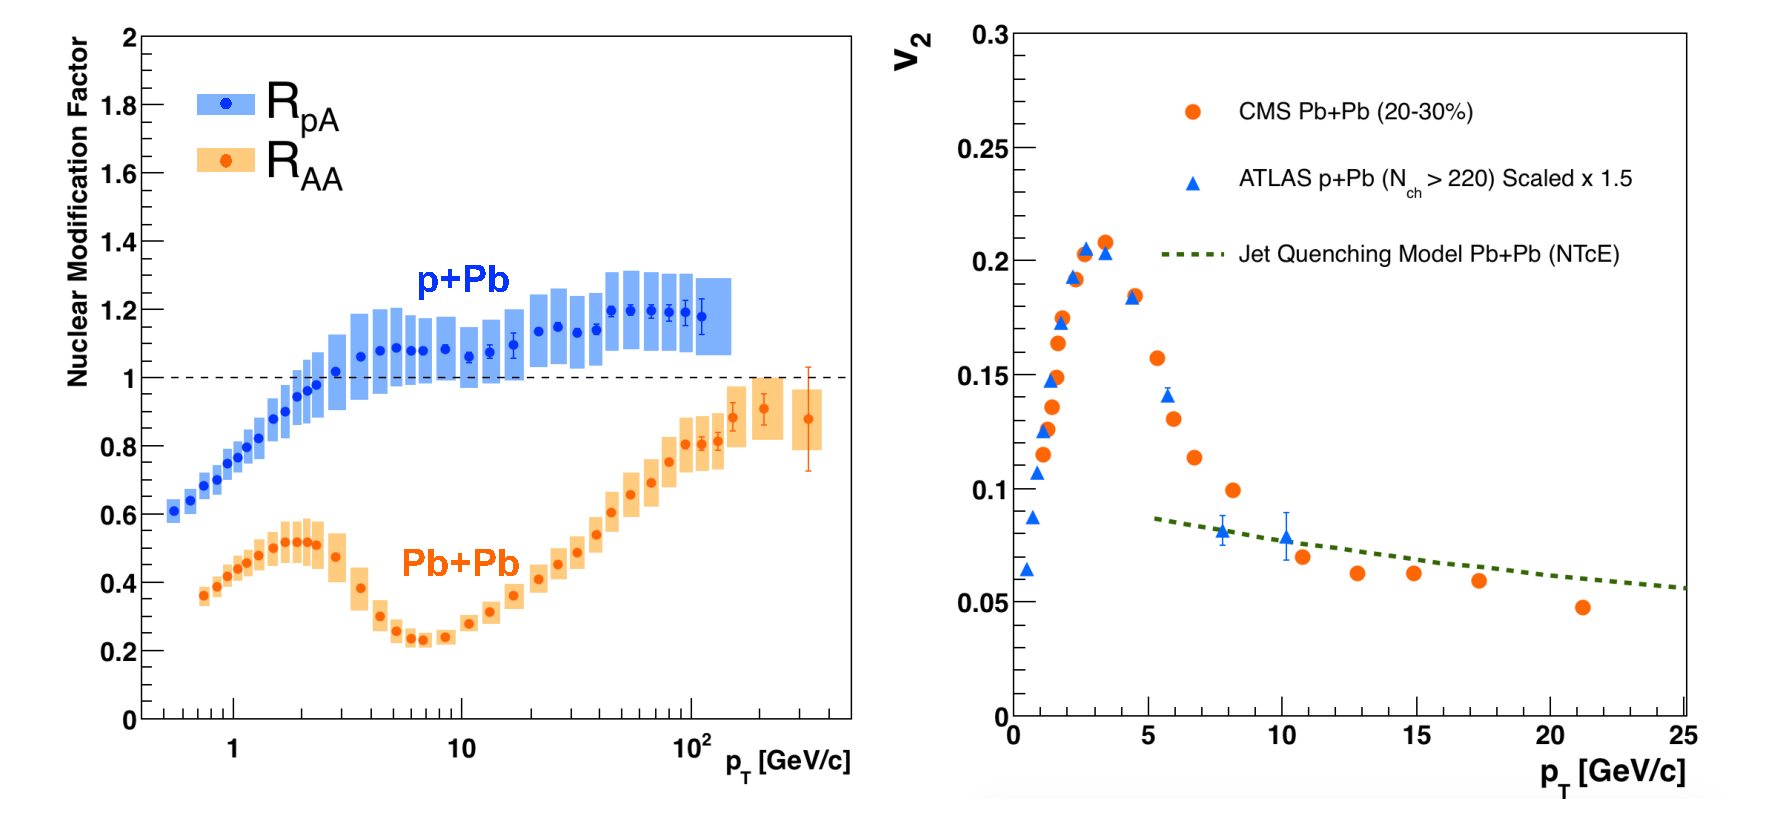
\includegraphics[width=0.9\textwidth]{pics/figure_ppb_jetquenching.pdf}
                \caption{{\it}The nuclear modification factor $R_\mathrm{pA}$ in \pPb collisions~\cite{Khachatryan:2016odn}. Compared to $R_\mathrm{AA}$  $R_\mathrm{pA}$ shows no sign of modification. 
                {\it right} The $v_2$ coefficient as a function of \pt{} in \PbPb and \pPb at the LHC~\cite{Aad:2014lta,Sirunyan:2017pan}. For shape comparison the \pPb results have been scaled up by a factor 1.5. The green dotted curve ~\cite{Zhang:2013oca} is from a jet quenching calculation where the anisotropy results from the directional dependence of the
energy loss, rather than hydrodynamic flow.}
                
	\label{fig:smallsystems3}
\end{figure}


%\begin{table}[htb]
%\centering
%\caption{Summary of observations in small system}
%\label{tab:Smallsystem}
%\begin{tabular}{ l | c | c | r }
%  Observable & PbPb & pPb & pp \\
%    \hline			
%  Jet RpA/RAA & Modified & No modification &  - \\
%  Hadron RpA/RAA & Modified & No modification &  -\\
%  Heavy flavors & & & \\
% % Jet quenching & Observed & No  \\
%  Jet shape & Broadening & No observations & - \\
%  Two-particle correlations & Ridge & Ridge & Ridge  \\
%  $v_2$ & Observed & Observed & Observed \\
%  Mass ordered flow & & & \\
%  Higher ordered harmonics & &  &\\
%  High $\pt{}$ $v_2$ & Observed & Maybe & - \\
%  \hline
%  \end{tabular}
%  \end{table}

\FloatBarrier
\subsubsection{Centrality determination in small systems}
\label{sec:smallsystemcentrality}
In lead-lead collisions the total multiplicity of the event is a good indicator of the geometric centrality of the collision~\cite{Abelev:2013qoq}. In proton-lead collisions the connection between multiplicity and centrality is less clear~\cite{Adam:2014qja}. In \pPb collisions the impact parameter is only loosely correlated to $N_\mathrm{part}$ or $N_\mathrm{coll}$. Hence, although one uses traditionally the term centrality to refer to these measurements, the relevant parameters are $N_\mathrm{part}$ and $N_\mathrm{coll}$~\cite{Adam:2014qja}.

\begin{figure}[b!]
\centering
            	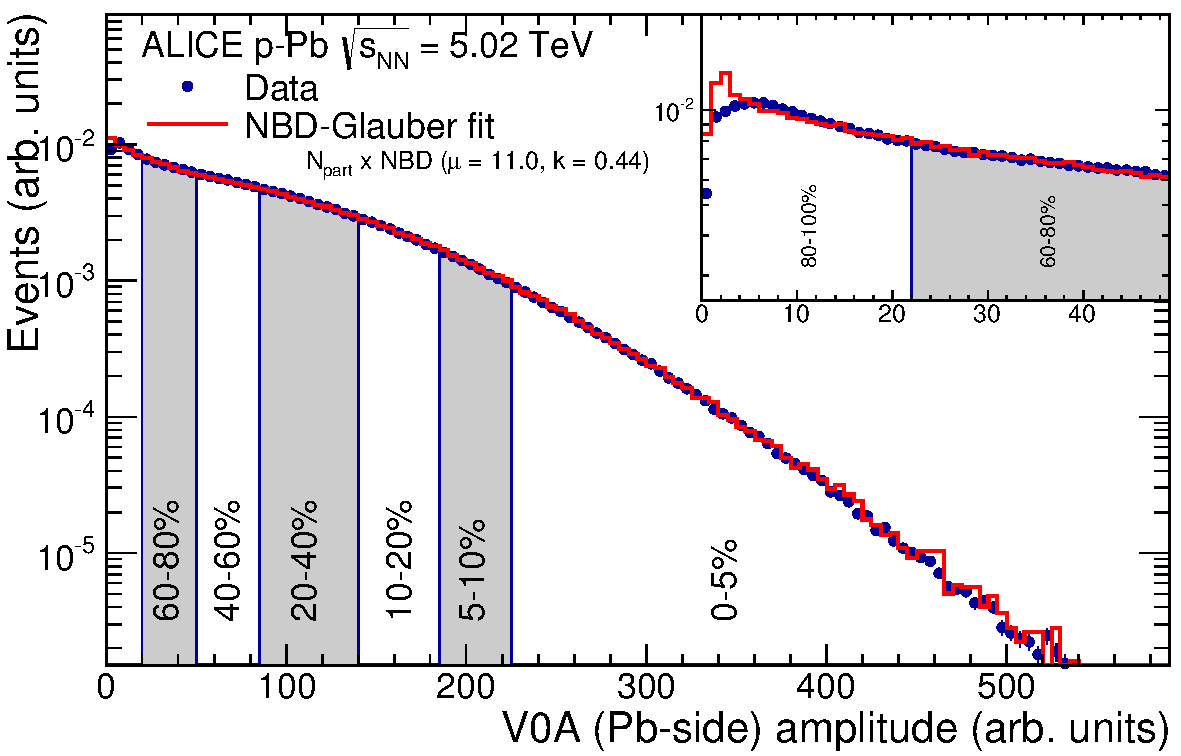
\includegraphics[width=0.50\textwidth]{pics/CentralitypPb}
                \caption{Distribution of the sum of amplitudes in the V0A hodoscopes (Pb-going), as well
as the NBD-Glauber fit. Centrality classes are indicated by vertical lines. The
inset shows a zoom-in on the most peripheral events.~\cite{Adam:2014qja}}
	\label{fig:pPbcentrality}
\end{figure}




As in \PbPb collisions the Glauber model~\cite{Miller:2007ri} is generally used to calculate geometrical quantities of \pPb collisions. In this model, the impact parameter $b$ controls the average number of participating nucleons $N_\mathrm{part}$ and the corresponding number of collisions $N_\mathrm{coll}$. It is expected that variations of the amount of matter overlapping in the collision region will change the number of produced particles, and parameters such as $N_\mathrm{part}$ and $N_\mathrm{coll}$ have traditionally been used to describe those changes quantitatively, and to relate them to \pp collisions. Figure ~\ref{fig:pPbcentrality} shows the measured V0A amplitude distribution in ALICE and the best NBD Glauber fit to the distribution~\cite{Adam:2014qja}.



%In practice centrality is determined in \pPb~collisions using the same methods as in \pbpb~collisions.

The problem in \pPb collisions is that fluctuations in multiplicity coming from for example hard scatterings are of the same order as the differences in multiplicity between centrality classes. In \PbPb collisions these multiplicity fluctuations have little influence on the centrality determination as the range of $N_\mathrm{part}$ or $N_\mathrm{coll}$ is large and both $P\left(M|N_\mathrm{part}\right)$ and $P\left(M|N_\mathrm{coll}\right)$ converge quickly to a Gaussian with a small width relative to the range of $N_\mathrm{part}$/$N_\mathrm{coll}$. This is illustrated in Figure~\ref{fig:pPbMult}. In practice selecting high multiplicity in \pPb one chooses not only large average $N_\mathrm{part}$, but also positive multiplicity fluctuations leading to deviations from the binary scaling of hard processes. These fluctuations are partly related to qualitatively different types of collisions. High multiplicity nucleon-nucleon collisions show a significantly higher mean transverse momentum. They can be understood either as harder collisions with larger momentum transfer $Q^2$ or as nucleon-nucleon collisions where multiple parton-parton interactions (MPI) take place. 

Of particular interest are estimators from kinematic regions that are causally disconnected after the collision. The measurement of a finite correlation between them unambiguously establishes their connection to the common collision geometry. Typically these studies are performed with observables from well separated pseudorapidity ($\eta$) intervals, e.g. at zero-degree (spectators, slow-nucleons, deuteron break-up probability) and multiplicity in the rapidity plateau.

One centrality selection that is argued not to induce a bias on the binary scaling of hard processes is provided by the energy measurement with the Zero Degree Calorimeters (ZDC) in ALICE, due to their large $\eta$-separation from the central barrel detectors. They detect the "slow" nucleons produced in the interaction by nuclear de-excitation processes or knocked out by wounded nucleons~\cite{Sikler:2003ef}.


\begin{figure}[htb]
\centering
            	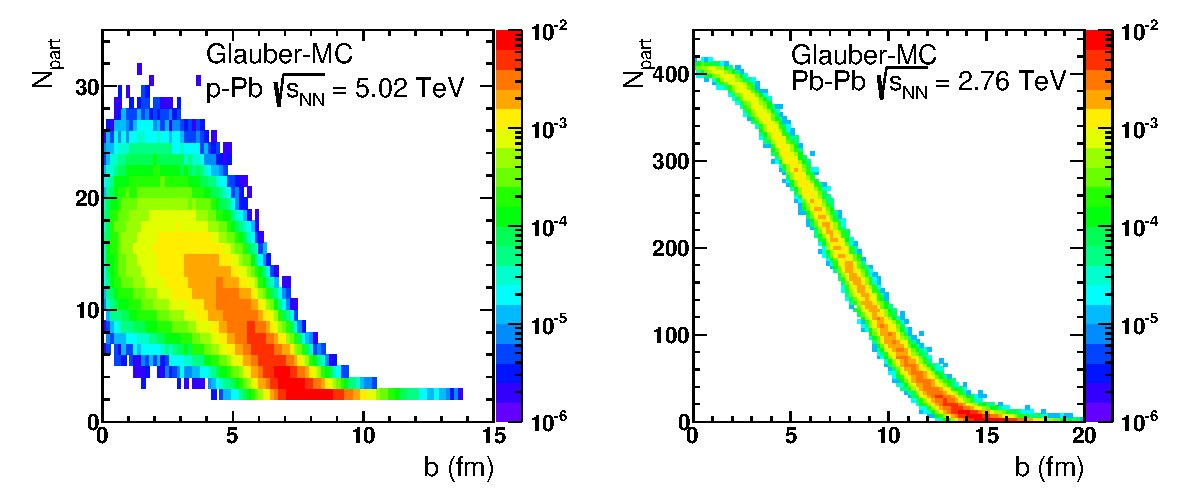
\includegraphics[width=0.7\textwidth]{pics/BNpart_Glau-10758.pdf}
            	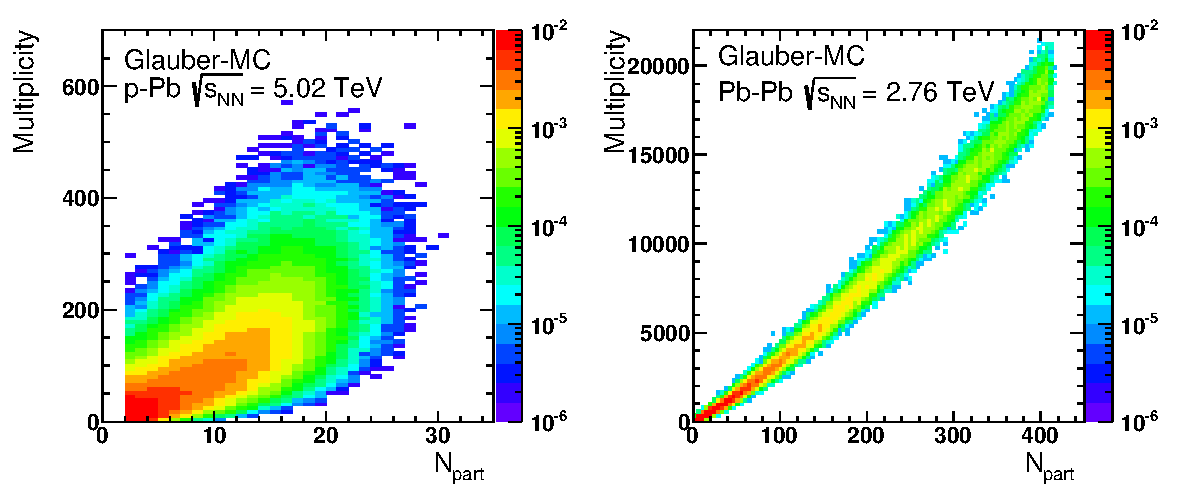
\includegraphics[width=0.7\textwidth]{pics/NpartMult_Glau-10759.pdf}
                \caption{Top: Scatter plot of number of participating nucleons versus impact parameter; Bottom: Scatter plot of multiplicity versus the number of participating nucleons from the Glauber fit for V0A. The quantities are calculated with a Glauber Monte Carlo of p-Pb (left) and Pb-Pb (right) collisions.~\cite{Adam:2014qja}}
	\label{fig:pPbMult}
\end{figure}


Additional kinematic biases exist for events containing high-$\pt{}$ particles, which arise from the fragmentation of partons produced in parton-parton scattering with large momentum transfer. Their contribution to the overall multiplicity increases with increasing parton energy and thus can introduce a trivial correlation between the centrality estimator and the presence of a high-$\pt{}$ particle in the event. For very peripheral collisions, the multiplicity range that governs the centrality for the bulk of soft collisions can represent an effective veto on hard processes. For the nuclear modification factor this would lead to $R_\mathrm{pPb} < 1$~\cite{Adam:2014qja}.

%{\color{red} More citations to final discussion?}


% !TEX root = thesis.tex
\section{Experimental Details}
\label{sec:exp}
\subsection{CERN}
The European Organization for Nuclear Research (CERN) is the largest particle physics laboratory in the world. CERN was founded in 1954. In 2019 CERN consists of 22 member states. Additionally CERN has contacts with a number of associate member states and various individual institutions. Some 12000 visiting scientists from over 600 institutions in over 70 countries come to CERN for their research. CERN itself is located near Geneva at the border of France and Switzerland and  itself employs about 2500 people.

The laboratory includes a series of accelerators, which are used to accelerate the particle beams used. A schematic view of the complex as of 2019 is shown in Figure~\ref{CernComplex}. In the framework of this thesis the main component is the Large Hadron Collider (LHC), the largest collider at CERN. LHC will be discussed in the chapter in more detail. Other accelerators in the series are used to inject the particle beam into LHC, but they are also used in itself for various experimental studies. 

The second largest accelerator is the super proton synchrotron (SPS). It is final step before the particle beam is injected into LHC. Commissioned in 1976, it was the largest accelerator at CERN until the the Large Electron-Positron Collider (LEP) was finished in 1989. Originally it was used as a proton-antiproton collider and as such provided the data for the UA1 and UA2 experiments, which resulted in the discovery of the W and Z bosons. At the moment there are several fixed target experiments utilising the beam from SPS. These study the structure (COMPASS) and properties (NA61/SHINE) of hadrons, rare decays of kaons (NA62) and radiation processes in strong electromagnetic fields (NA63). Additionally the AWAKE and UA9 experiments are used for accelerator research and development. 

-PS

\begin{figure}
\centering
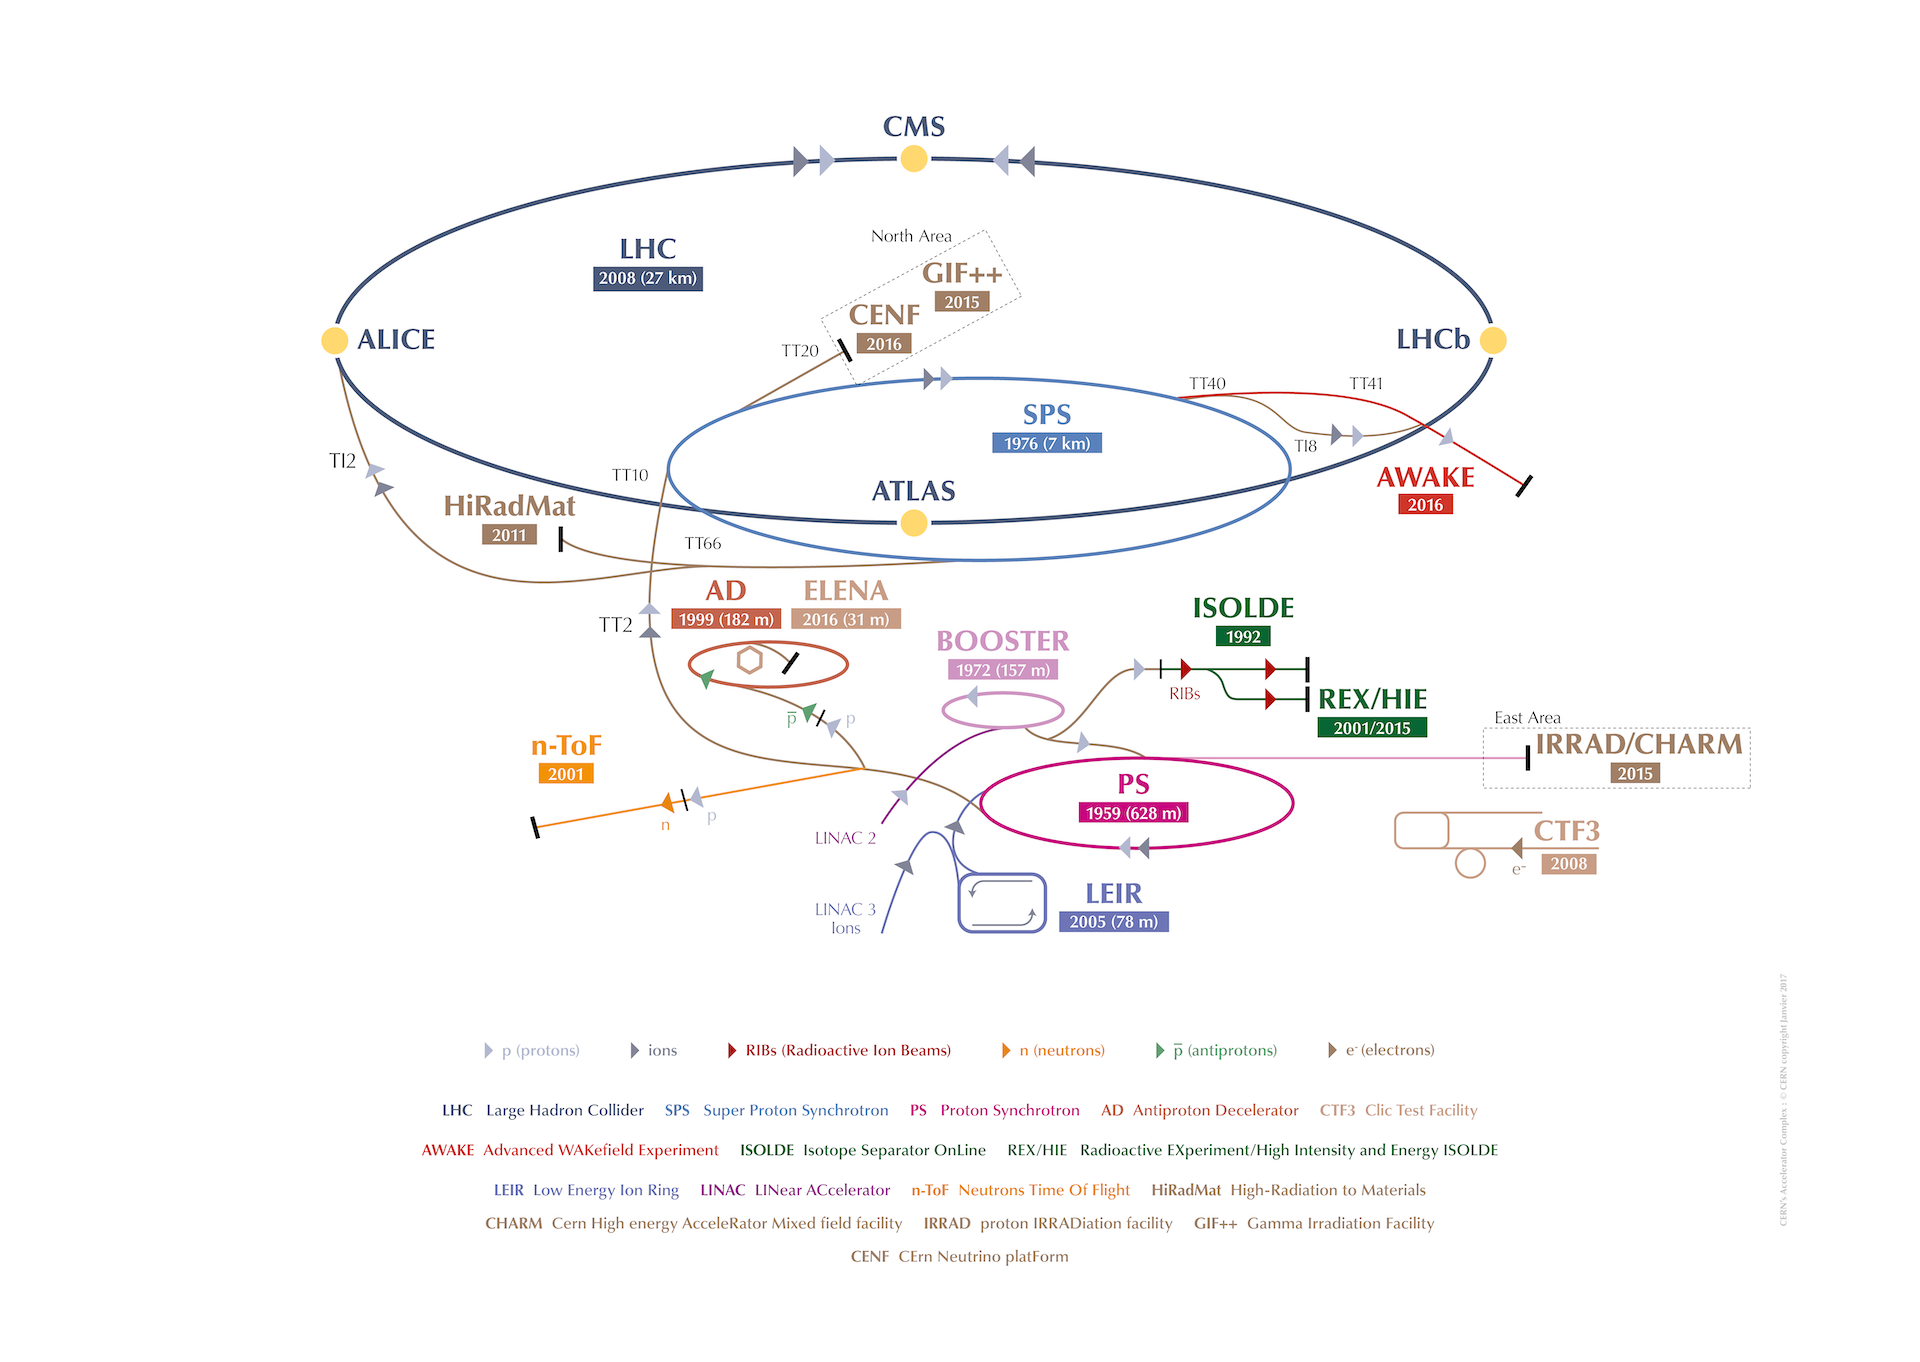
\includegraphics[width=0.9\textwidth]{pics/CernCollidersSmall}
\caption[CERN collider complex]{ A schematic view of the accelerator complex at CERN. Before particles can be injected into the LHC they require a series of preliminary? acceletarors. Until 2018 protons start their journey in LINAC2 (Linear Accelerator) and continue through the Booster, Proton Synchrotron (PS) and Super Proton Synchrotron (SPS). Between 2019 and 2020 LINAC2 will be replaced by LINAC4~\cite{CernComplex}}

\label{fig:CernComplex}
\end{figure}
\subsection{Large Hadron Collider}
\label{sec:lhc}
The Large Hadron Collider (LHC) is the largest accelerator at CERN and the largest particle collider ever built. The LHC is designed to accelerate protons up to an energy of 8\tev and lead ions up to 2.76\tev per nucleon~\cite{LHC}. The design luminosity of the LHC is $10^34 \unit{cm^{-2}s^{-1}}$. In 20xx it achieved a record peak luminosity of xxx. For lead beams the design luminosity is xxx. All this is achieved with a ring of 26.7 km, that consists of 1232 superconducting dipole magnets that keep particles in orbit. 

The particles are accelerated through the use of radio-frequency (RF) cavities. The RF are build such that the electromagnetic waves become resonant and build up inside the cavity. Charges passing through the cavity feel the overall force and are pushed forward along the accelerator. As they consist of electromagnetic waves, the field in the RF cavity oscillates. Thus particles must enter the cavity at the correct phase of oscillation to receive a forward push. When timed correctly, the particles will feel zero accelerating voltage when they have exactly the correct energy. Particles with higher energies will be decelerated  and particles with lower energies will be accelerated. This focuses particles in distinct bunches. The RF oscillation frequency at the LHC is 400.8 MHz. Thus  RF "buckets" are separated by 2.5 ns. However only 10 \% are actually filled with particles, so the bunch spacing in the LHC is 25 ns, at a bunch frequency of 40 MHz.

With 7 TeV proton beams the dipole magnets used to bend the beam must produce a magnetic field of 8.33 T. This can be only achieved through making the magnets superconducting, which requires cooling them down with helium to a temperature of 1.9 K. The 1232 dipole magnets make up roughly 2/3 of the LHC circumference. The remaining part is made up of RF cavities, various sensors and higher multipole magnets used to keep the beam focused. The most notable of these are the 392 quadrupole magnets.

The LHC is divided into octants, where each octant has a distinct function. Octants 2 and 8 are used to inject beam into the LHC from SPS. The 2 beams are crossed in octants 1,2,5 and 8. The main experiments are built around these crossing points. Octants 3 and 7 are used for beam cleansing. This is achieved through collimators that scatter particles with too high momentum or position offsets off from the beam. The RF cavities used for acceleration are located in octant 4 and octant 6 is used for dumping the beam. The beam dump is made up of two iron septum magnets, one for each beam, that will kick the beam away from machine components into an absorber when needed. 


\subsubsection{LHC experiments}
As of 2018 there are four main experiments at the LHC; ALICE, ATLAS, CMS and LHCb and three smaller ones LHCf, TOTEM and MoEDAL. ALICE will be covered in section ~\ref{sec:alice}. 

ATLAS (A Toroidal LHC ApparatuS) and CMS (Compact Muon Solenoid) are the two largest experiments at the LHC. They are both multipurpose experiments designed to be sensitive to many different possible new physics signals. The biggest discovery made by these so far is the discovery of the Standard Model Higgs boson, which was simultaneously published by the experiments in 2012 ~\cite{Atlashiggs, CMShiggs}.

The LHCb (LHC beauty) experiment ~\cite{LHCb} is made for studying the bottom (beauty) quark. Main physics goals include measurement of the parameters of CP violation with decays of hadron containing the bottom quark. One of the most important results published by LHCb is the first measurement of $B_s^0\rightarrow \mu^+ \mu^-$ decay, which was found to be in line with the Standard Model.

In addition to the four large experiments there are three smaller experiments along the LHC ring. LHCf (LHC forward) is located at interaction point 1 with ATLAS. It aims to simulate cosmic rays by the particles thrown forwards by the collisions in ATLAS.

TOTEM (TOTal Elastic and diffractive cross section Measurement) is located near the CMS experiment at point 5. This allows it to measure particles emerging from CMS with small angles. The main goals is to measure the total, elastic and inelastic cross-sections in pp collisions~\cite{TOTEM}.

The MoEDAL (Monopole and Exotics Detector At the LHC) experiment is located at the interaction point 8 together with the LHCb experiment. MoEDAL tries to measure signatures of hypothetical particles with magnetic charge, magnetic monopoles.




\subsection{ALICE}
\label{sec:alice}


\begin{figure}[htb]
\centering
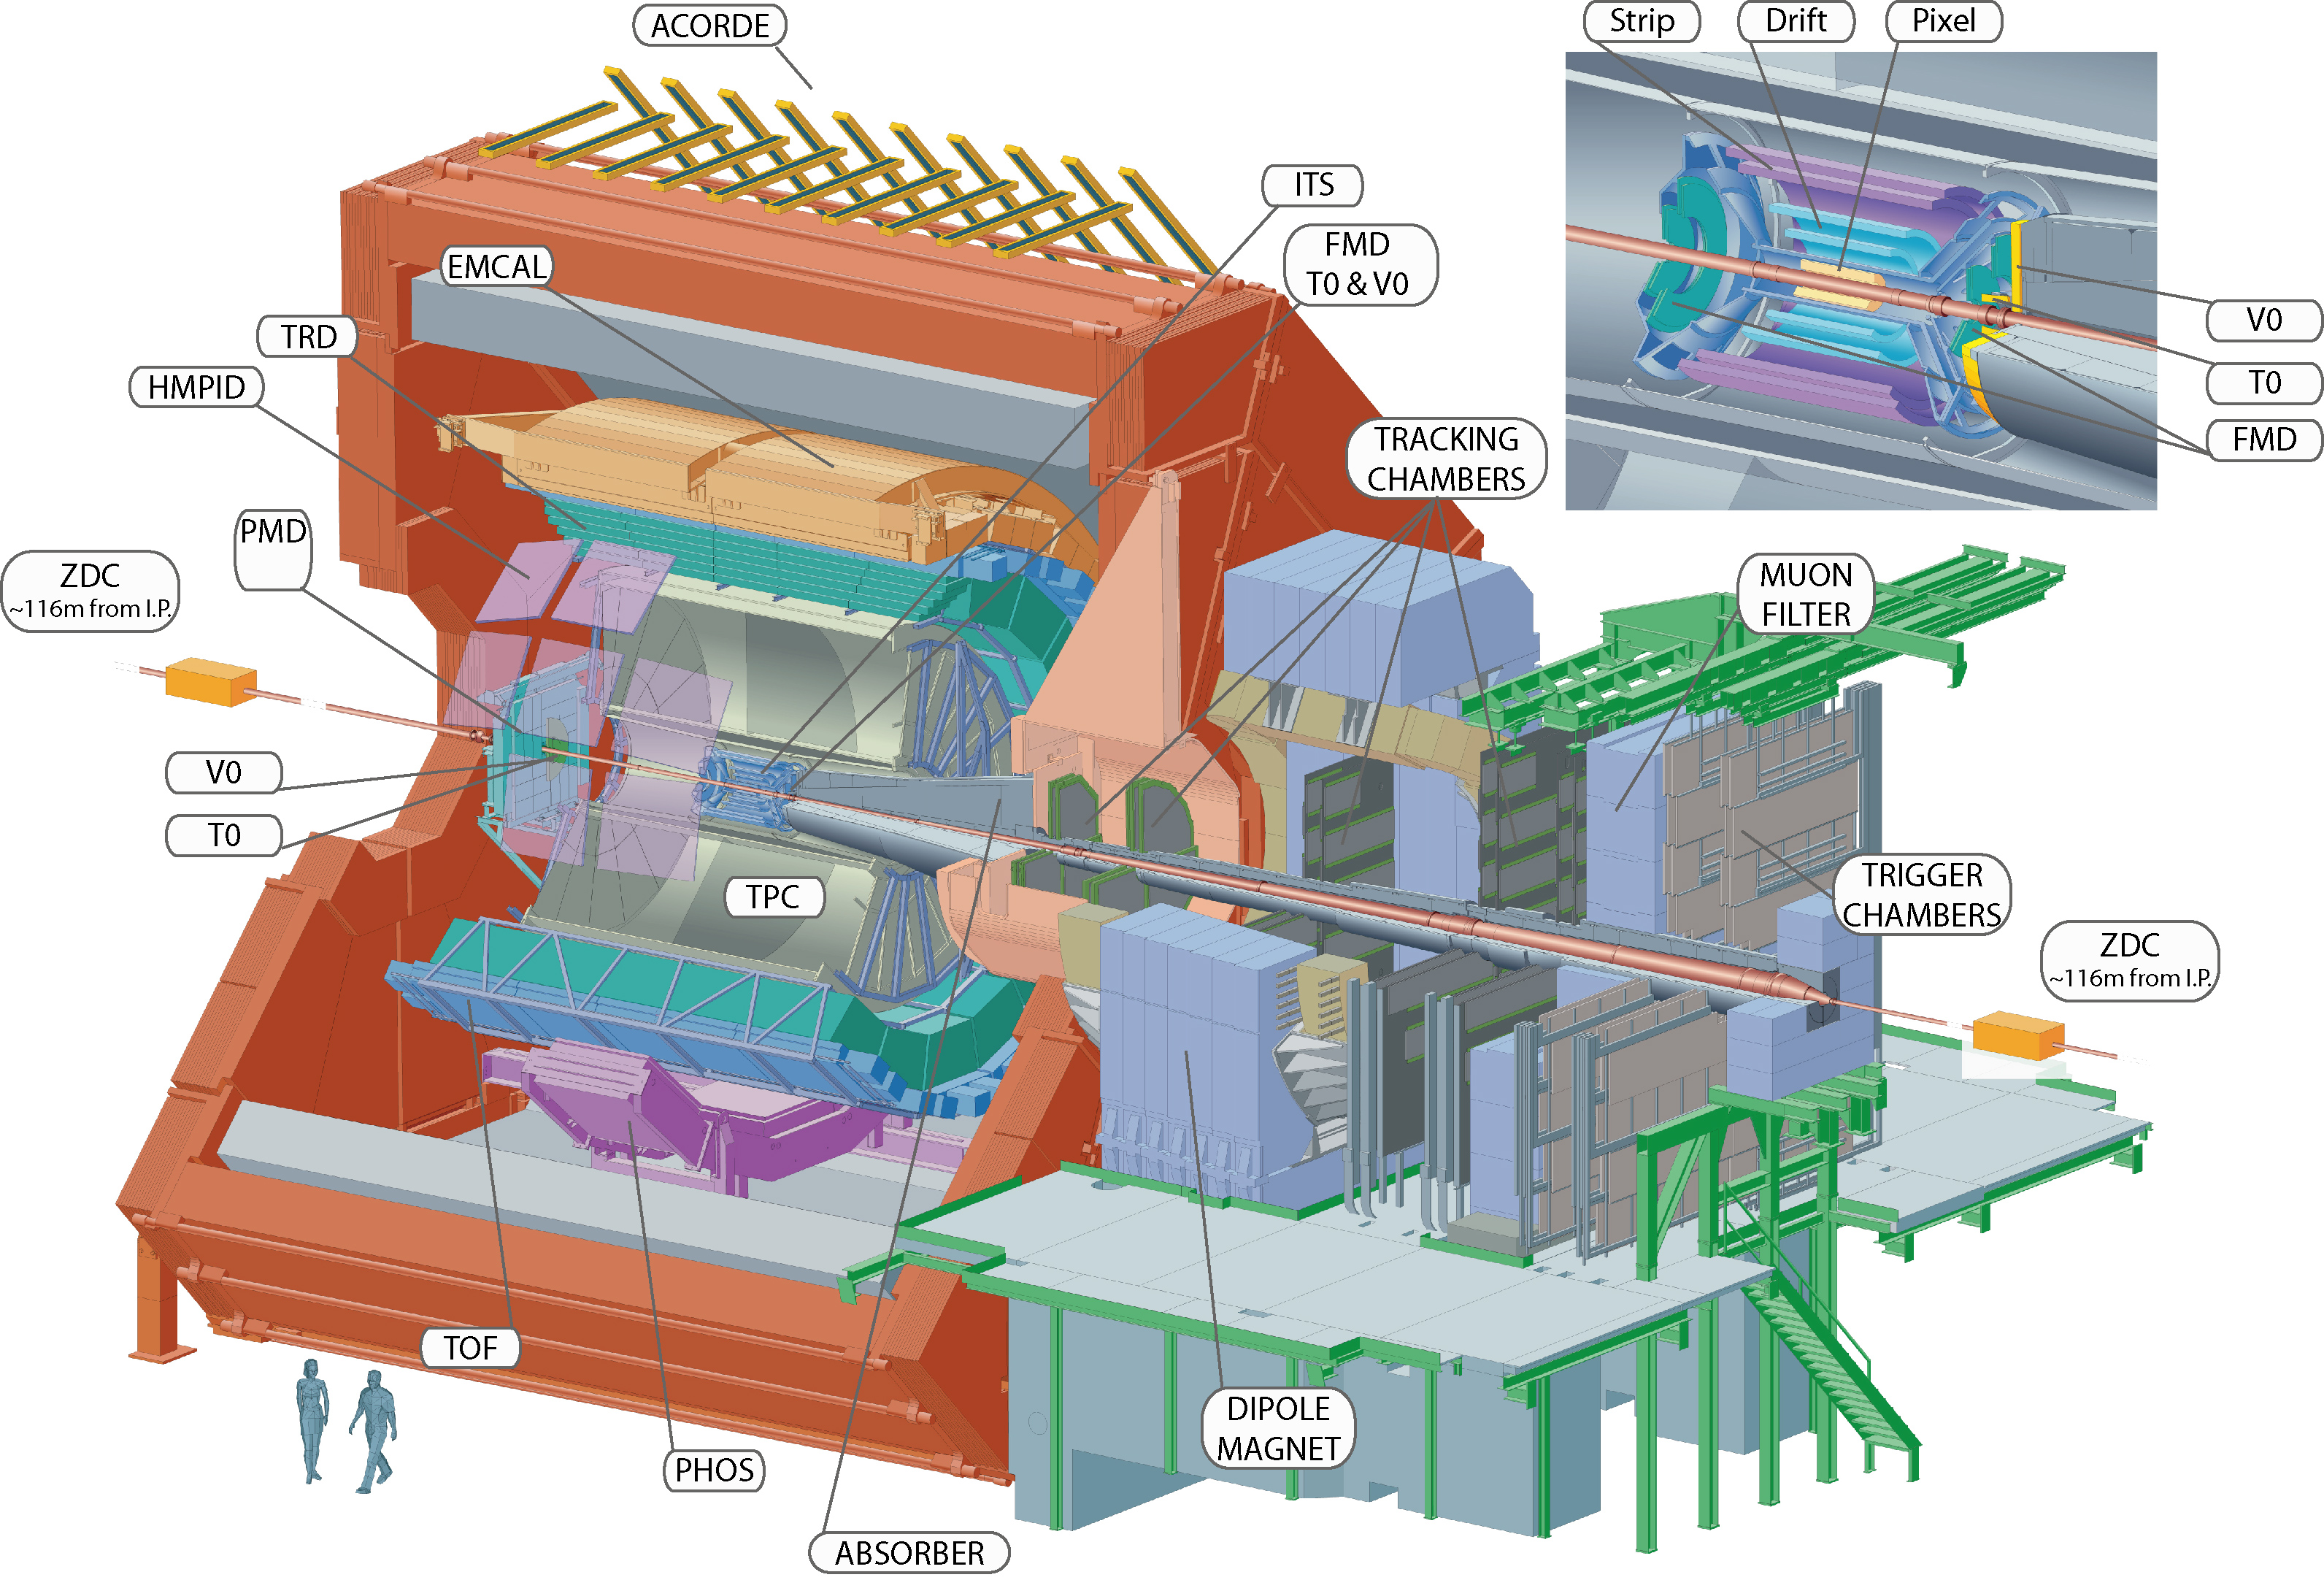
\includegraphics[width=0.95\textwidth]{pics/2012-Aug-02-ALICE_3D_v0_with_Text.jpg}
\caption[ALICE]{Schematic view of ALICE}
\label{fig:alice}
\end{figure}

ALICE (A Large Ion Collider Experiment)~\cite{ALICE} is the dedicated heavy ion experiment at the LHC. ALICE was designed to cope with the expected very high multiplicity environment of heavy ion collisions. The design allows measurement of a large number of low momentum tracks. The different detector subsystems are optimised to provide high momentum resolution and excellent particle identification capabilities over a broad range of momentum.

A schematic view of the ALICE detector in 2018 is presented in Figure ~\ref{fig:alice}. This section will go through the composition of ALICE as it has been during run 2 between 2014 and 2018. The detector will go through significant upgrades during Long Shutdown 2 in 2019-2020. As in all the major high energy physics experiments the positioning of the detectors follows a layered structure. Closest to the interaction point are the tracking detectors. The main task of these detectors is to locate the position of the primary interaction vertex accurately and to record the tracks of charged particles. To achieve this they need a very good spatial resolution close to the interaction point. Tracking detectors do not significantly alter the tracks of traversing particles. Thus they can be located in the innermost layers.

Calorimeters are designed to stop any particles hitting them and use the absorption to measure the energy of the particles. Thus they must be located behind the tracking detectors. ALICE has two separate calorimeter systems, the electromagnetic calorimeters measure mainly electrons and photons, while the muon detection system measures muons.


\subsubsection{Tracking}
\begin{figure}[htb]
\centering
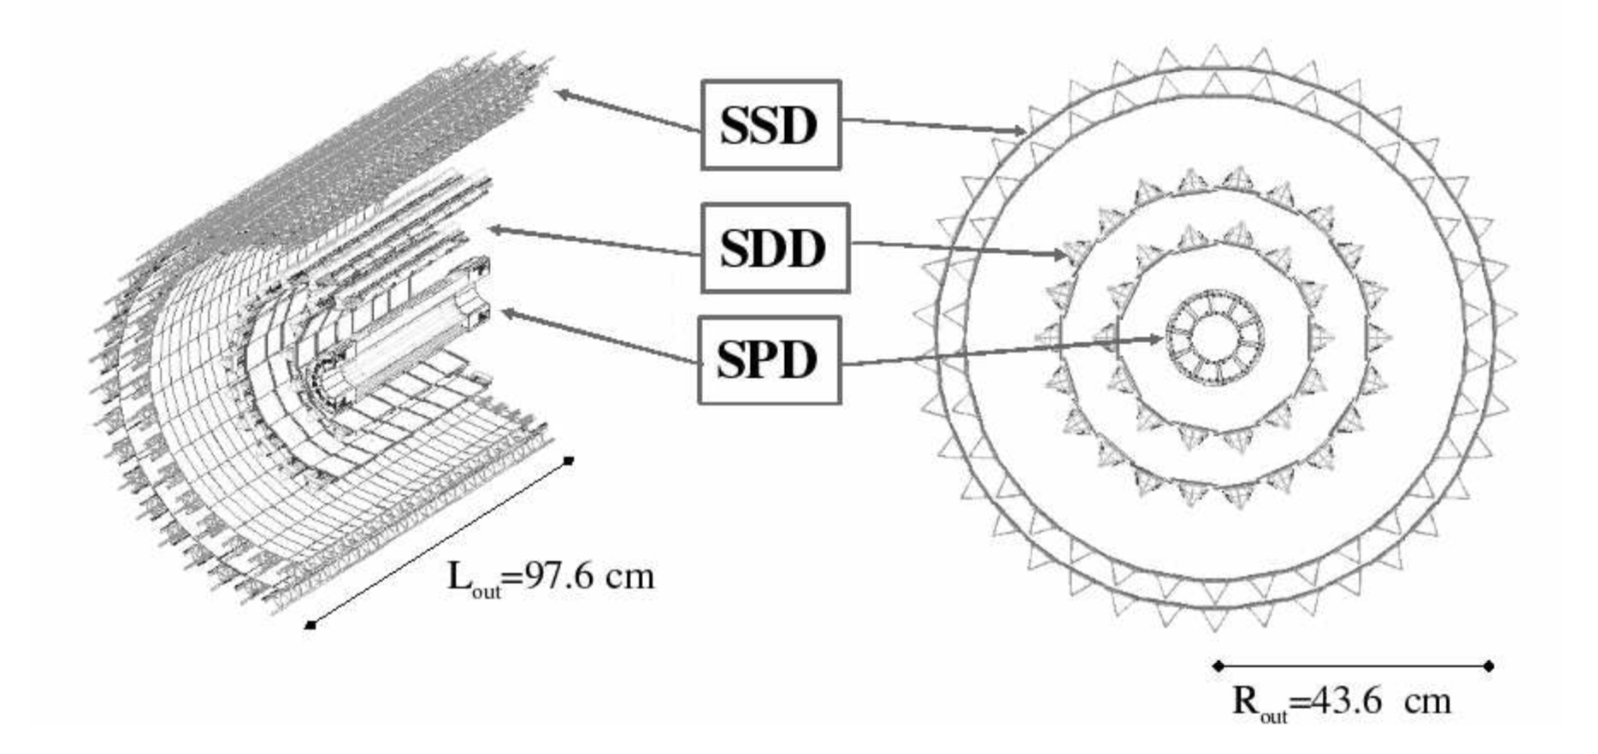
\includegraphics[width=0.95\textwidth]{pics/AliceITS}
\caption[ITS]{Schematic view of ALICE Inner Tracking System}
\label{fig:its}
\end{figure}


The main design guideline for the tracking detectors in ALICE was the requirement to have good track separation and high granularity in the high multiplicity environment of heavy ion collisions. Before LHC was built the wildest estimates put the particle density at 8000 charged particles per unit of rapidity~\cite{}. In reality the particle density turned out to be significantly smaller, about 1600 charged particles per rapidity unit.~\cite{}

The main tracking detector in ALICE is the Time Projection Chamber (TPC), discussed in more detail in section ~\ref{sec:TPC}

Between TPC and the beam pipe there is an array of six layers of silicon detectors, called the inner tracking system (ITS)~\cite{ITS}. The main tasks of the ITS are to locate the primary vertex with a resolution better than 100 $\mu m$, to reconstruct the secondary vertices from decaying particles, to track and identify particles with momenta below 200 $\mev$ and to compliment the momentum and angle measurements of TPC. During long shutdown 2 in 2019-2020 the entire ITS will be replaced~\cite{ITSupgrage}. As of 2018 the two innermost layers are made of the silicon pixel detector (SPD). As it's the closest detector to the interaction point it requires are very high spatial resolution. Thus the choice of pixel technology is natural. In heavy ion collisions the particle density is around 50 particles per $cm^2$. 

The next two layers are the silicon drift detector (SDD), which is made out of homogeneous neutron transmutation doped silicon. It is ionized when a charged particle goes through the material. The generated charge then drifts to the collection anodes, where it is measured. The maximum drift time in SDD is about 5 $\mu s$ This design gives very good multitrack capabilities and provides two out of the four $\nicefrac{dE}{dx}$ samples in the ITS.

The two remaining layers in the ITS are the silicon strip detector (SSD). The strips work in a similar way as silicon pixels, but by itself one layer only provides good resolution in one direction. Combining two crossing grids of strips provides 2 dimensional detection. Each charged particle will hit two intervening strips. The position of the hit can be deduced from the place where the strips cross each other.

\subsubsection{TPC}
\label{sec:TPC}
Time projection chamber (TPC) is a cylindrical detector filled with $ 88 m^3$ of $\mathrm{Ne-CO_2}$ (90/10 \%) gas mixture. The gas is contained in a field cage that provides an uniform electric field of $400 \nicefrac{V}{cm}$ along the z-axis (along the beam direction). Charged particles traversing through the TPC volume will ionise the gas along their path. This liberates electors that drift towards the end plates of the cylinder. 

The field cage is separated into two detection volumes by the central high voltage electrode. Both sides have a drift length of 2.5 m and inner/outer diameters of 1.2/5 m. This means the central electrode must provide a maximum potential of 100 kV to achieve the design field magnitude. The maximum time required for electrons to drift through the chamber is about 90 $\mu s$.

When electrons reach the end of the main cylinder they enter the readout chambers. The readout section of both sides consists of 18 outer chambers and 18 inner chambers. Each of them are made of multiwire proportional chambers with cathode pad readout. This design is used in many TPCs before. During Long Shutdown 2 in 2019-2020, the multiwire chambers will be replaced by Gas Electron Multipliers (GEMs, see section \ref{sec:tpcupgrade}).

The relatively slow drift time of 90 $\mu s$ is the limiting factor for the luminosity ALICE can take. The occupancy of the TPC must be kept in a manageable level. 


\subsubsection{TPC upgrade}
\label{sec:tpcupgrade}
\begin{figure}[htb]
\centering
\includegraphics[width=0.95\textwidth]{pics/alice-tpc-schematic}
\caption[TPC]{Schematic view of ALICE Time Projection Chamber}
\label{fig:tpc}
\end{figure}
During long shutdown 2 in 2019-2020 ALICE will go through significant modifications. The goal is to be able have continuous readout ~\cite{aliceupgrade} in heavy ion collisions at an interaction rate of 50 kHz. I have made a personal contribution to the quality assurance of the new GEM readout of TPC.

ALICE will add a new Forward Interaction trigger (FIT) to replace the V0 and T0 detectors. 

Additionally the current inner tracking system (ITS) will be completely replaced. The current layered structure with three different technologies will be replaced by an all pixel detector with significantly reduced pixel size. Additionally the first layer will be brought closer to the beam pipe. The new ITS will have better tracking efficiency and  better impact parameter resolution. 

The muon detection will be complimented by the Muon Forward Tracker (MFT)~\cite{mft}. Based on the same technology as the new ITS, MFT will be placed before the hadron absorber that sits in front of the existing muon spectrometer. MFT should significantly increase the signal/background ratio in heavy quark measurements.

Many subdetectors will make small improvements to enhance the readout rate. The central trigger processor will be replaced and ALICE will introduce a new framework $O^2$ that combines both online data acquisition and offline analysis.

The detector restricting the readout the most at the moment is the TPC. The current wire chamber based system  limits the readout rate to 3.5 kHz. To achieve the 50 kHz readout rate goal the wire chambers will be replaced by a Gas Electron Multiplier (GEM) based system.

TPC has a total of 36 inner and 36 outer readout chambers. Each of these will consist of 4 layers of GEM foils. The inner chambers will only have one foil for each layer. The outer chambers are separated into three sections, each with its own layer of foils. Each gem foil is made up of a 50 $\mathrm{\mu m}$ thick resistive capton layer, coated on both sides by $5 \mathrm{\mu m}$ thick layers of copper. Each foils is separated into a number (20-24) of distinct active areas. The active areas are pierced quite densely, they have 50-100 holes in the area of a single $\mathrm{mm^2}$. The density of holes changes from layer to layer. The two middle layers of foils have a larger (double) pitch (smaller hole density) while the top and bottom layers have a smaller (normal) pitch (larger hole density).

The holes have a conical shape which they acquire during a two step chemical etching process. 

The working principle of these foils is based on electrodynamics. {\color{red} elaborate}There is a large potential difference (140-400 V) applied to the two sides of the foil, which results in large field in each hole. This acts both as a lens and an amplifier for the electrons. The amplification happens inside the holes where the field is the strongest. 

As opposed to wire chambers, which typically have one voltage setting, a GEM-based detector requires several independent voltage settings: there is a drift voltage which drives the electrons from the ionisation point to the GEM, an amplification voltage, and an extraction voltage that brings electrons from the GEM exit to the readout plane. 

The GEMs are designed to minimise ion backflow to allow continuous, ungated and untriggered readout.

The purpose of the multilayered structure is to reduce the ion backflow~\cite{}; not only one layer of GEM foils will be installed, but a 4 layer stack. In the stack there are 2 standard pitch GEM foils, where the pitch size, i.e. the separation of the holes inside a foil is around 140 $\mu m$, and 2 large pitch GEM foils, there the hole spacing is two times larger, 280 $\mu m$. The two outer layers will have standard pitch and the two middle layers have large pitch. The middle layers with large pitch serve as extra insulator against the ion backflow. Additionally the setup allows operating individual GEM foils at lower voltages and still have an increase in the gain of a few orders of magnitude.

~\cite{TPCupgrade}

\subsubsection*{Quality Assurance of the GEM foils}
The GEM foils are produced at CERN, where they will undergo a basic QA (QA-B) procedure, that includes

\begin{itemize}
\item Coarse optical inspection to see any major defects, holes, cuts and discoloured regions
\item Short-term leakage current measurement
\end{itemize}

Any problems found in the basic inspection are documented for later cross-checking.


The advanced quality assurance (QA-A) is performed in two centers, one in the Helsinki Institute of Physics (HIP) and one in the Wigner Research Centre in Budapest. The QA-A procedure includes the following measurements

\begin{itemize}
\item Long-term leakage current measurement
\item High-resolution optical scanning
\item Gain uniformity check (In Budapest)
\end{itemize}

In the procedure foils are classified according to a traffic light system. Red means the foil didn't pass the basic selection criteria and thus cannot be used. Yellow means it might be usable and green means that the foil passed all evaluations.

\subsubsection{Optical scanning}
The etching process is a delicate one; many things can go wrong, that are not visible by eye in the coarse optical inspection. It is expected that the hole parameters are connected with the foil's electric properties~\cite{}, so a precise optical measurement can help in classifying the foils. For example, smaller holes create more intense and focused fields, which would result in larger amplification of their avalanche electrons, i.e. the local gain would be larger.

The foils are scanned with the help of a scanning robot. The setup along with most of the software was developed at the Detector Laboratory of the University of Helsinki~\cite{}

Each image is a false colour superposition of two images, one with foreground illumination and one with background illumination. In this way one can observe the three relevant diameters of the foil, the top, middle and bottom diameters. The background light highlights the middle holes, while the foreground illumination captures either the top or the bottom depending on the orientation of the foil as the foils are scanned from both sides. Fig.~\ref{fig:gemscan}

The setup takes images with area about $\unit[11.3]{mm} \times \unit[8.5]{mm}$, corresponding to 2560 by 1920 pixels, resulting in a total of 2000-3500 individual images for both sides of a GEM foil, depending on its type. The images are fed into neural network classifier, which identifies the holes, finds defects and extracts the hole parameters by fitting ellipses to the recognised contours. Thus every individual hole can be measured, which otherwise would be completely unfeasible as even the smallest of foils has about 10 million holes.

\begin{figure}
%\includegraphics
\caption{An example image taken of a GEM foil with false colors.}
\label{fig:gemscan}
\end{figure}

\subsubsection*{Long term HV measurement of the GEM foils}
After the optical scanning, the foils are subjected to a long term ( 5-12 hours) high voltage leakage current measurement. Each segment of the GEM foil is connected to a high voltage and the leakage current is measured separately for each segment, by the connected picoamper-meter (pA-meter)~\cite{}. The accepted leakage current in each segment is \unit[0.16]{nA}, foils with larger values are discarded. 

\subsubsection*{Gain scan}
A small subset of the foils were put through a gain scan. The gain scan could only be performed in the QA-A centre of Budapest. As the time required to scan 1 foil was several days, the gain scan couldn't be performed even for all foils in Budapest. 

The gain scan uses charged particles provided by a $\mathrm{^{55} Fe}$ source, which was placed above the foil. It emits X-ray photons with an energy of \unit[5.9]{keV}. The photons will convert to electrons in the gain scanner's $\mathrm{Ar+CO_2}$ gas mixture, either via photoelectric effect or via Compton Scattering. There electrons travel a few microns in the gas, ionising the gas along their path.

Below the GEM frame, there is a multiwire proportional pad, with perpendicular wires with a resolution of \unit[4]{mm} in $x$ and \unit[3]{mm} in $y$. Amplification is measured both with (HV) and without (reference) voltage over the GEM foil. The HV measurement is divided with the reference measurement, which results in the gain map of the GEM.

\subsubsection*{Gain correlations}

\subsubsection{Particle identification}
One guiding principle in the design of ALICE was to achieve good particle identification (PID) over  a large part of phases space and for several different particle types. In ALICE there are several detectors taking part in the identification of particles. 

One of the particle identification detectors is the transition radiation detector (TRD)~\cite{trd}. Its main task is identifying electors with momenta larger than 1 \gev. Transition radiation is produced when highly relativistic particles traverse the boundary between to media having different dielectric constants. The average energy of the emitted photon is approximately proportional to the Lorentz factor $\gamma$ of the particle, which provides an excellent way of discriminating between electrons and pion. ALICE TRD is made of a composite layer of foam and fibres. The emitted photons are then measured in six layers of Xe/CO2 filled time expansion wire chambers. 

The time of flight  (TOF) detector uses a very simple physics principle, i.e. calculating the velocity of the particle using the time of flight between two points. Combining this with the momentum of particle, obtained from the tracking detectors, one can calculate the mass of the particle, which identifies particles. The TOF detector consists of multigap resistive wire chambers. These are stacks of resistive plates spaced equally. They allow time of flight measurements in large acceptance with high efficiency and with a resolution better than 100 ps. 

The third specific particle identification detector is the high momentum particle identification (HMPID) detector. The HMPID uses a ring imaging Cherenkov counter to identify particles with momenta larger than 1 \gev. Particles moving through a material faster than the speed of light in the material will produce Cherenkov radiation. The velocity of the particle determines the angle at which the radiation is emitted. Measuring this angle gives the velocity of the particle. This can be again used to calculate the mass of the particle, if the momentum is known. In HMPID the material is a liquid radiator and the photons are measured with multiwire proportional chambers in conjunction with photocathodes. 

In addition to the specific particle identification detectors, the general purpose tracking detectors can be used for identification through the use of specific energy loss of charged particles traversing through a medium and the transition radiation emitted by charged particles when crossing the boundary between two materials. 

$\nicefrac{\mathrm{d}E}{\mathrm{d}x}$ measurements are provided by the last four layers of the ITS detector, i.e. the SDD and the SSD, thanks to their analog readout.~\cite{ALICEpid} ITS provides particle identification in the low $\pt{}$ region, up to $~ 1 \gev$, and pions reconstructed in the standalone mode can be identified down to $~100 \mev$. Similar to ITS the TPC detector provides specific energy loss measurements. TPC can identify charged hadrons up to $p_T ~ 1-2 \gev$ as well as light nuclei, He3 and He4.


\subsubsection{Electromagnetic Calorimeter}
Calorimeters are designed to measure the energy of particles. Electromagnetic calorimeters specialise in detecting particles that interact primarily through the electromagnetic interaction, namely photons and electrons. They are required in many neutral meson and direct photon analyses. In addition the energy information enhance jet measurements.

ALICE has two electromagnetic calorimeters, the photon spectrometer (PHOS)~\cite{PHOS} and the electromagnetic calorimeter (EMCal)~\cite{emcal}. PHOS is a homogeneous calorimeter that consists of scintillating $\mathrm{PbWO_4}$ crystals, which generate a bremsstrahlung  shower and produce scintillation light. The energy of the particle determines the amount of light produced. To improve the charged particle rejection, PHOS includes a charged particle veto detector (CPV)~\cite{cpv}. PHOS is built to have a very fine granularity, making it well suited for measuring direct photons and neutral mesons.

EMCal is a sampling calorimeter. It consists of layers of lead and scintillator tiles. The lead tiles produce the shower and scintillator tiles the light. The signal is then read with wavelength shifting fibres. The acceptance of EMCal in the azimuthal angle is $ 80\deg < \phi < 187 \deg$. During long shutdown 1 in 2013-2015, EMCal was extended with the di-jet calorimeter (DCal) ~\cite{DCAL}, giving an additional acceptance region of $ 260\deg < \phi < 320 \deg$. This provides partial back-to-back coverage. In comparison to PHOS, EMCal has coarser granularity, but a significantly larger acceptance, making it suitable for jet physics.

\subsubsection{Forward detectors}
ALICE includes a few small and specialised detectors of importance. The event time is determined with very good precision (< 25 ns) by the T0 detector~\cite{T0}. T0 consists of two sets of Cherenkov counters that are mounted around the beam pipe on both sides of the interaction point. T0 gives the luminosity measurement in ALICE.

Another small detector in the forward direction is the V0 detector~\cite{V0}. This consists of two arrays of segmented scintillator counters located at $-3.7 < \eta < -1.7$ and $ 2.8 < \eta < 5.1$. V0 is used as a minimum bias trigger and for rejection of beam-gas background. Particle multiplicity in the forward direction can be related to the event centrality. Thus V0 is the main detector used in centrality determination in PbPb collisions.

The multiplicity measurement of V0 is complimented by the forward multiplicity detector (FMD)~\cite{FMD}. FMD includes five rings of silicon strip detectors that make up the FMD. FMD gives acceptance in the range $-3.4 < \eta < -1.7$ and $ 1.7 < \eta < 5.0$.

During long shutdown 2 in 2019-2020, V0 and T0 will be replaced by the Fast Interaction Trigger (FIT) detector~\cite{FIT}. For historical reasons elements of FIT are also referred to as V0+ and T0+. FIT will allow centrality, event plane, luminosity and interaction time determination in the continuous readout mode, that ALICE will operate in after 2020.

For photon multiplicity measurement ALICE has the photon multiplicity detector (PMD) ~\cite{PMD}. PMD uses two planes of gas proportional counters with a cellular honeycomb structure. PMD gives the multiplicity and spatial distribution of photons in the region $2.3 < \eta < 3.7$.

On top of the ALICE magnet there is an array of 60 large scintillators called the ALICE cosmic ray detector (ACORDE) ~\cite{acorde}. ACORDE is used as a trigger for cosmic rays for calibration and alignment. 

The only hadronic calorimeters in ALICE are the zero degree calorimeters (ZDC)~\cite{zdc}, which are located next to the beam pipe in the machine tunnel about 116 m from the interaction point. There are two sets of calorimeters. One is made of tungsten, specialising in measuring neutrons, while the other, made of brass, is specialised in measuring protons. In heavy ion and especially in proton-lead collisions, ZDC gives information about the centrality of the event. ZDC is meant to detect spectators, i.e. parts of the colliding ions that do not take part in the interaction. If there are more spectators, the collisions is likely to be more peripheral.

A new detector installed during the long shutdown 1 is the ALICE diffractive detector (AD)~\cite{AD}. AD consists of two assemblies, one in each side of the interaction point, both made of two layers of scintillators. These assemblies are situated about 17 m and 19.5 m away from the interaction points. The pseudorapidity coverage is $-6.96 < \eta < -4.92 $ and $4.78 < \eta < 6.31$. AD greatly enhances ALICE's capability for diffractive physics measurements that require a large pseudorapidity gap.

\subsubsection{Muon spectrometer}
Outside the main magnet, ALICE has a spectrometer dedicated to measuring muons~\cite{MuonSpectro}. In heavy ion physics muons are mainly used to measure the production of the heavy quark resonances $\nicefrac{J}{\psi}, \Psi^{'}, \Upsilon, \Upsilon^{'}$ and $\Upsilon^{''}$.

The muon spectrometer consists of three parts, the absorber, the muon tracker and the muon trigger. The absorber is meant to remove the hadronic background as efficiently as possible. After the absorber there are ten plates of thin cathode strip tracking stations with high granularity, the muon tracker. After the muon tracker there is a layer of iron to filter out any remaining particles, other than muons. The muon trigger is located behind this layer. The trigger consists of four resistive plate chambers. 
\subsubsection{Trigger}
\subsubsection*{EMCAL trigger}


% !TEX root = thesis.tex
\section{Event and track selection}
\label{sec:selection}
The $\sqrtSnnE{5.02}$ $\pPb$ ($1.3 \cdot 10^{8}$ events, $\mathcal{L}_{\mathrm{int}} = \unit[62]{nb^{-1}}$) collisions were recorded in 2013 by the ALICE detector~\cite{aliceDetector}. The details of the performance of the ALICE detector during LHC Run~1 (2009-2013) are presented in Ref.~\cite{alicePerformance}.

%For the 2010 $\pp$ collisions, the minimum bias (MB) triggered events are required to have at least one hit from a charged particle traversing the SPD or either side of the V0. 
%The pseudorapidity coverage of the SPD is $|\eta| < 2$ in the first layer and $|\eta| < 1.5$ in the second layer. %Combining this with the acceptance of the V0, the particles are detected in the range $-3.7 < \eta < 5.1$. The minimum %bias trigger definition 



%For the $\pp$ collisions, similar track cuts as in Ref.~\cite{ALICE:2011ac} are used: at least two hits in the ITS are required, one of which needs to be in the three innermost layers, and 70 hits out of 159 are required in the TPC. In addition, the distance of the closest approach (DCA) of the track to the primary vertex is required to be smaller than $\unit{2}{cm}$ in the beam direction. In the transverse direction, a $\pt{}$ dependent cut DCA $< \unit{0.0105}{cm} + \unit{0.035}{cm} \cdot \pt{}^{-1.1}$ is used, where $\pt{}$ is measured in units of $\GeVc$. These track cuts are tuned to minimize the contamination from secondary particles.

%In $\pPb$ collisions the tracks are selected following the hybrid approach~\cite{hybridExplanation}. In this method tracks with at least one hit in the SPD and at least two hits in the whole ITS are always accepted. In addition, tracks with fewer than two hits in the ITS or no hits in the SPD are accepted, but only if an additional vertex constraint is fulfilled. In addition, the distance of the closest approach (DCA) of the track to the primary vertex is required to be smaller than $\unit{3.2}{cm}$ in the beam direction and smaller than $\unit{2.4}{cm}$ in the transverse direction. This approach is not affected by dead regions ins SPD. Thus it produces an azimuthal angle ($\varphi$) distribution that is as uniform as possible. The momentum resolutions of the two classes of particles are comparable up to $\pt{} \approx 10\;\GeVc$, but after that, tracks without ITS requirements have a worse resolution~\cite{alicePerformance,aliceBackgroundFluctuation}.




\subsection{Event selection}
This analysis uses both a minimum bias trigger and an EMCal based trigger to select the analysed events. 
%The V0 detector~\cite{forwarddetectorsTdr} provides the information for event triggering. The V0 detector consists of two scintillator hodoscopes that are located on either side of the interaction point along the beam direction. It covers the pseudorapidity region $-3.7 < \eta < -1.7$ (V0C) and $2.8 < \eta < 5.1$ (V0A).
 For the 2013 $\pPb$ collisions minimum bias events are required to have signals in both V0A and V0C. The timing difference between the two stations is also used to reduce the contamination of the data sample from beam-gas events~\cite{alicePerformance}. 

EMCal is used to provide the jet trigger used in triggered datasets. EMCal can be used to trigger on single shower deposits or energy deposits integrated over a larger area. Latter case is used for jet triggers. The EMCal trigger definition in the 2013 $\pPb$ collisions requires an energy deposit of either \unit[10]{\gev}  for the low threshold trigger or \unit[20]{\gev} for the high threshold trigger in a $32\times32$ patch size. Triggers, V0 and EMCal are discussed in more detail in sections~\ref{sec:forward},~\ref{sec:trigger} and~\ref{sec:emcal}. 

\subsection{Track reconstruction}
%\setlength{\emergencystretch}{0em}

The analysis uses charged tracks that are reconstructed with the Inner Tracking System (ITS)~\cite{aliceITS} and the Time Projection Chamber (TPC)~\cite{aliceTPC}. These are discussed in sections~\ref{sec:tracking} and~\ref{sec:TPC}. A detailed overview of track reconstruction in ALICE can be found from~\cite{alicePerformance}. 

The track reconstruction procedure is shown in Figure~\ref{fig:tracking}. The figure shows only one track, but in reality the reconstruction has to deal with many tracks. The main reconstruction of tracks starts in TPC. There are 159 tangential pad rows in the TPC readout chambers. The track reconstruction starts from the outermost layer and the hits are paired with hits in the next layer inwards, taking into account a proximity cut. When this track finding procedure hits the innermost pad row in TPC, this information is used as an initial seed for the track finding in ITS. Similar procedure of pairing adjacent layers with a proximity cut is repeated in ITS.

After the reconstruction of tracks in ITS is completed, all the tracks are extrapolated to their point of closest approach to the preliminary interaction vertex. Then the second track fitting step begins, this time starting from the interaction point and proceeding outwards. A Kalman filter~\cite{Fruhwirth:1987fm} technique is used to do the new fit using the hits found in the previous stage. This time the tracks are matched also to the other detectors in the central barrel beyond TPC. When this step is complete, a final refit from the outermost TPC pad rows towards the interaction point is performed. The final track parameters come from this refit. 

With the final track parameters the primary vertex can be determined with better accuracy than with only SPD information. The tracks are extrapolated to the nominal beam line and a weighted average of the points of closest approach determines the accurate primary vertex position.

The final step of the track reconstruction is the determination of the secondary vertices. For this, all the tracks whose distance of closest approach (DCA) to the primary vertex is larger than a defined minimum value %(?? \unit{mm} in \pPb)
are selected. For these tracks, points of closest approaches are determined for pairs of tracks. If the tracks are sufficiently close to each other and show characteristics of short lived particle decays, these points are identified as secondary vertices. 

\begin{figure}[h]
%\input{figures/tikz/tracking}
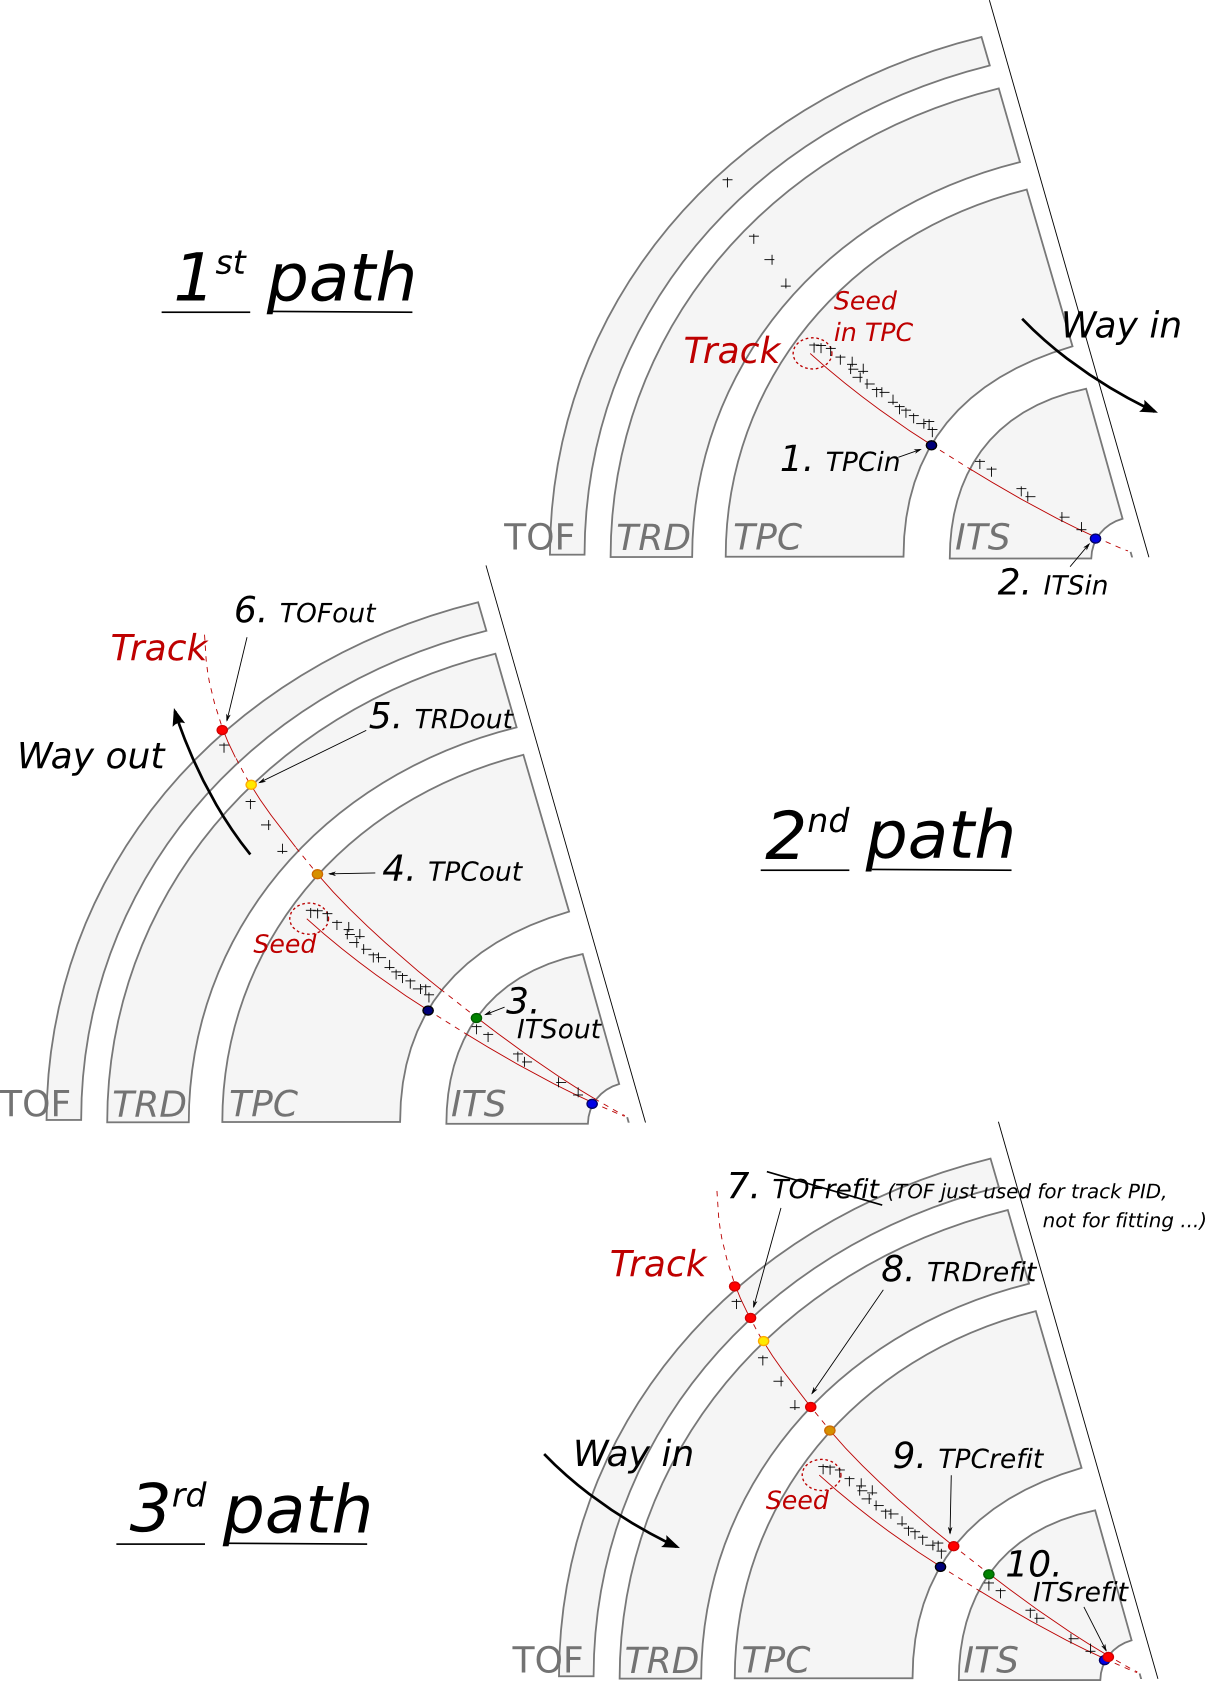
\includegraphics[width=0.9\textwidth]{pics/Schema-PcpTrackingALICE.png}
\caption{Principles of tracking in the ALICE experiment, showing the three successive paths allowing to build a track and refine its parameters. Numbers ranging from 1 to 10 mention the bits that are activated in case of success during the propagation of the Kalman filter at the considered stage. Figure from ~\cite{Maire:1984041}}
\label{fig:tracking}
\end{figure}

Combining the information from the ITS and the TPC provides a resolution ranging from $1$ to $10\,\%$ for charged particles with momenta from $0.15$ to $\unit[100]{\GeVc}$. For tracks without the ITS information, the momentum resolution is comparable to that of ITS+TPC tracks below transverse momentum $\pt{} = \unit[10]{\GeVc}$, but for higher momenta the resolution reaches $20\,\%$ at $\pt{} = \unit[50]{\GeVc}$~\cite{alicePerformance,aliceBackgroundFluctuation}. 


\subsubsection*{Track selection}
In $\pPb$ collisions the tracks are selected following the hybrid approach~\cite{hybridExplanation} which ensures a uniform distribution of tracks as a function of azimuthal angle ($\varphi$). The parameters in the approach are summarised in Table~\ref{tab:hybrid}. 

The first requirements are on the quality of the track fit in ITS and TPC. The ITS requirement only removes tracks that are clear outliers. For TPC the requirement is much more strict. For step 1 it is required that a track has 3 out of the 6 possible hits in ITS, one of which must be in the SPD. In step 2 this is replaced by an additional vertex constraint, where the primary vertex itself is added as a point to the track to improve the momentum resolution.

For the TPC, 70 crossed pad rows out of the maximum 159 is required. This measures the effective track length inside the TPC. This takes into account the possibility of having pad rows missing in the middle of the track due to charge in these clusters being below the threshold for some reason. Additionally it is required that the ratio between crossed rows and findable clusters is at least 0.8. Findable clusters are defined as the number of geometrically possible clusters which can be assigned to a track, taking into account dead zones due to chamber boundaries and limited $\eta$-acceptance. For both steps of the hybrid cut it is required that the fraction of clusters shared with several tracks is less than 40\%.

%Additionally we only accept tracks with $\left| \eta \right| < 0.8$ to avoid border effects ot the TPC acceptance $\left| \eta \right| < 0.9$ 

The remaining cuts are meant to make sure that the measured tracks are really produced in the primary collision. A track might gain a kink due to a particle scattering decay. The particle after such a kink, a kink daughter, is rejected in the cuts, as it no longer describes the properties of the primary collisions. The final cuts are on the distance of closest approach (DCA) of the track to primary vertex. To have confidence that the track comes from the primary collision, the track must be close enough to the primary vertex. The cuts are different for the distance along ($\mathrm{DCA}_{z}$) and perpendicular to ($\mathrm{DCA}_{xy}$) the beam axis.


\begin{table}
\caption{Parameters in the hybrid track cut}
\label{tab:hybrid}
\begin{tabular}{c | c | c}
Track Cut & Step 1 & Step 2 \\
\hline
$\chi^2$ / ITS cluster & < 36 & < 36 \\
$\chi^2$ / ITS cluster & < 4 & < 4 \\
Hits in ITS & 3 & 0 \\
ITS hit requirements & 1 in SPD & No requirement \\
Vertex constraint & No & Yes \\
Number of crossed rows in TPC  & 70 & 70 \\
TPC crossed rows over findable clusters & > 0.8 & > 0.8 \\
Fraction of shared TPC clusters & < 0.4 & < 0.4 \\
Kink daughters & Rejected & Rejected \\
$\mathrm{DCA}_{xy}$ & < \unit[3.2]{cm} & < \unit[3.2]{cm} \\
$\mathrm{DCA}_{z}$ & < \unit[2.4]{cm} & < \unit[2.4]{cm} \\
Other & & Rejected by step 1 \\
\end{tabular}
\end{table}



%The momentum resolutions of the two classes of particles are comparable up to $\pt{} \approx 10\;\GeVc$, but after that, tracks without ITS requirements have a worse resolution~\cite{alicePerformance,aliceBackgroundFluctuation}.



%These detectors are located inside the large solenoidal magnet, that provides a homogeneous magnetic field of \unit[0.5]{T}. Tracks within a pseudorapidity range $|\eta| < 0.9$ over the full azimuth can be reconstructed. 

%The ITS is made up of the innermost Silicon Pixel Detector (SPD), the Silicon Drift Detector (SDD) and the outermost Silicon Strip Detector (SSD). Each of these consists of two layers. The TPC is a cylinder filled with gas. Gas is ionised along the path of charged particles. Liberated electrons drift towards the end plates of the cylinder where they are detected. 


\FloatBarrier
\subsection{Cluster selection}
Neutral particles used in jet reconstruction are reconstructed by the Electromagnetic Calorimeter (EMCal)~\cite{Cortese:2008zza}. The EMCal covers an area with a range of $|\eta| < 0.7$  in pseudorapidity and $ 100 \deg $ in azimuth. EMCal is complimented with the Dijet Calorimeter (DCal)~\cite{DCAL} and Photon Spectrometer (PHOS)~\cite{PHOS} that are situated opposite of the EMCal in azimuth. PHOS covers 70 degrees in azimuth and $\left| \eta \right| < 0.12$. The DCal is technologically identical to EMCal. The DCal coverage spans over 67 degrees in azimuth, but in pseudorapidity the mid region is occupied by the PHOS. In between PHOS and DCal active volumes, there is a gap of 10 cm. DCal is fully back-to-back with EMCal.

\begin{table}[tb] 
\centering
\caption{Parameters used in the EMCal clusteriser}
\label{tab:clusters}
\begin{tabular}{| c | c |}
Setting & Value \\
Clusteriser seed & 0.2 \unit{\mev} \\
Clusteriser cutoff & 0.05 \unit{\mev} \\
Cells in cluster & > 1 \\
Track matching radius & 0.025 \\
Fiducial cut & 1 tower \\
Exotic cut & 0.97 \\
Minimal cluster Energy & 0.3 \unit{\gev}
%Maximum pair asymmetry & 0.8 \\
\end{tabular}
\end{table}

The clusters used in the analysis were obtained from the EMCal clusteriser. The parameters used in the clusteriser are summarised in Table~\ref{tab:clusters}. The clusteriser  searches for a tower with energy deposit greater than a defined seed energy and merges all surrounding (sharing a side) towers with energy deposit higher than a defined threshold. In the next step all towers sharing a side with already included towers are added, again requiring that the energy deposits exceeds the threshold. The algorithm can identify local minima and halts the clustering in case that the neighbouring tower energy is higher. Already clustered towers are removed from the pool, so one tower can only be clustered once. 

Highly energetic calorimeter hits should spread into several towers as the electromagnetic shower evolves. However, some clusters with high energy have their energy located in a single tower. These are believed to come from a slow neutron hitting the APD readout of the towers. They are referred to as exotic clusters. The measure of exoticity is denoted as 
\begin{equation}
1 -\frac{E_\mathrm{cross}}{E_\mathrm{max}},
\end{equation}

\noindent where $E_\mathrm{max}$ is the energy in the most energetic tower and $E_\mathrm{cross}$ is the sum of the four towers neighbouring the most energetic one. The closer this is to 1, the more exotic the cluster is and the larger the probability that it is fake. Cut of 0.97 has been adopted as default for analyses using EMCal, including the one presented in this thesis. Any clusters above this cut are removed.

A method of matching the cluster position to TPC track extrapolation is used to suppress charged hadron contribution to hits in EMCal. Tracks identified by the tracking detectors are extrapolated close to the EMCal surface, where the closest cluster is found and the track extrapolation is continued until reaching the same depth as the cluster. The remaining distance in between the extrapolated track and the cluster is then used to reject hadronic hits. Clusters matched to charged tracks are removed from the analysis as well as clusters being identified as fake. 








%The combination of charged tracks with  $\pt{} > \unit[0.15]{\GeVc}$ and neutral particles with $\pt{} > \unit[0.30]{\GeVc}$ is used to construct jets. 


%\subsection{statistics}
%Number of jets in different datasets and with different jet finders is shown in Table~\ref{tab:stats}. Background statistics for number of background cones (number of jets minus number of discarded cones) are shown in Table~\ref{tab:bgstats}. Ratio of background cones to number of jets is shown in Table~\ref{tab:bgratio}. The likelihood of having to discard a jet from background calculation is about 1-2\%.
%\begin{table}[h]
%\caption{Number of found jets by dataset and jet $\pt{}$ bin}
%\tiny
%\begin{tabular}{c | c | c | c | c | c | c | c | c | c}
%Jet $\pt{}$   &     5-10 & 10-20  & 20-30 & 30-40 & 40-60 & 60-80 & 80-100 & 100-150 & 150-500 \\
%MBFullR04 & 4969393 & 621753 & 32552 & 5584 & 1974 & 310 & 90 & 37 & 5 \\
%MBFullR05 & 4750567 & 826598 & 42373 & 5543 & 1719 & 276 & 73 & 29 & 3 \\
%MBChargedR04 & 3144538 & 673419 & 37783 & 4121 & 1009 & 148 & 36 & 12 & 1 \\
%MBChargedR05 & 2229247 & 175763 & 7961 & 1270 & 410 & 61 & 12 & 3 \\
%TriggeredFullR04 & 187557 & 115927 & 78138 & 51317 & 39262 & 8621 & 2409 & 1167 & 171 \\
%TriggeredFullR05 & 99991 & 77147 & 48612 & 34325 & 28104 & 6342 & 1726 & 794 & 104 \\
%TriggeredChargedR04 & 37411 & 29945 & 18186 & 13148 & 11142 & 2517 & 675 & 326 & 44 \\
%TriggeredChargedR05 & 433155 & 175031 & 54789 & 19776 & 10626 & 1983 & 457 & 194 & 15 \\
%\end{tabular}
%\label{tab:stats}
%\end{table}
%
%\begin{table}[h]
%\caption{Number of background cones used in perpendicular cone background calculation}
%\label{tab:bgstats}
%\tiny
%\begin{tabular}{c | c | c | c | c | c | c | c | c | c}
%Jet $\pt{}$     &   5-10 & 10-20  & 20-30 & 30-40 & 40-60 & 60-80 & 80-100 & 100-150 & 150-500 \\
%MBFullR04 & 4947583 & 617895 & 32357 & 5548 & 1965 & 310 & 90 & 37 & 5 \\
%MBFullR05 & 4710217 & 815461 & 41584 & 5439 & 1698 & 273 & 73 & 29 & 3 \\
%MBChargedR04 & 3117495 & 661106 & 36739 & 4014 & 988 & 144 & 36 & 12 & 1 \\
%MBChargedR05 & 2195286 & 172919 & 7860 & 1249 & 406 & 61 & 12 & 3 \\
%TriggeredFullR04 & 186574 & 115376 & 77949 & 51216 & 39196 & 8603 & 2405 & 1167 & 171 \\
%TriggeredFullR05 & 99102 & 76462 & 48320 & 34216 & 28038 & 6334 & 1722 & 794 & 103 \\
%TriggeredChargedR04 & 37160 & 29543 & 17988 & 13099 & 11129 & 2515 & 675 & 326 & 44 \\
%TriggeredChargedR05 & 313421 & 140707 & 45229 & 16243 & 8709 & 1604 & 377 & 154 & 14 \\
%\end{tabular}
%\end{table}
%
%\begin{table}[h]
%\caption{Ratio of background cone number to number of jets}
%\label{tab:bgratio}
%\tiny
%\begin{tabular}{c | c | c | c | c | c | c | c | c | c}
%MBFullR04 & 99.56\% & 99.38\% & 99.40\% & 99.36\% & 99.54\% & 100.00\% & 100.00\% & 100.00\% & 100.00\% \\
%MBFullR05 & 99.15\% & 98.65\% & 98.14\% & 98.12\% & 98.78\% & 98.91\% & 100.00\% & 100.00\% & 100.00\% \\
%MBChargedR04 & 99.14\% & 98.17\% & 97.24\% & 97.40\% & 97.92\% & 97.30\% & 100.00\% & 100.00\% & 100.00\% \\
%MBChargedR05 & 98.48\% & 98.38\% & 98.73\% & 98.35\% & 99.02\% & 100.00\% & 100.00\% & 100.00\% \\
%TriggeredFullR04 & 99.48\% & 99.52\% & 99.76\% & 99.80\% & 99.83\% & 99.79\% & 99.83\% & 100.00\% & 100.00\% \\
%TriggeredFullR05 & 99.11\% & 99.11\% & 99.40\% & 99.68\% & 99.77\% & 99.87\% & 99.77\% & 100.00\% & 99.04\% \\
%TriggeredChargedR04 & 99.33\% & 98.66\% & 98.91\% & 99.63\% & 99.88\% & 99.92\% & 100.00\% & 100.00\% & 100.00\% \\
%TriggeredChargedR05 & 72.36\% & 80.39\% & 82.55\% & 82.13\% & 81.96\% & 80.89\% & 82.49\% & 79.38\% & 93.33\% \\
%\end{tabular}
%\end{table}
%
%


\clearpage
\section{Analysis method}
\label{sec:methods}
\subsection{Jet Finding}
The analysis uses reconstructed jets as estimates of the original parton. Jet reconstruction essentially combines nearby tracks into jets. 

Collisions between hadrons are never as clean as electron-electron collisions. Even for a proton-proton collision there are participant partons, that will produce a soft background in addition to the hard scattering products. Jet reconstruction must deal with this soft background. The reconstruction is never perfect, one can have uncorrelated tracks that get included in the jet and some tracks originating from the parton are missed by the reconstruction. There are several methods to perform the reconstruction, all of which require some kind of size parameter, which cuts out jet participants too far from the jet axis. The tracks that are grouped into a jet are referred to as jet constituents. 

In each collision event, the jets are reconstructed using FastJet~\cite{fastjet} with the anti-$\kt{}$ algorithm~\cite{antikt}. Jets for R=0.4 are selected in $\left| \eta \right| < 0.25 $ to satisfy the fiducial acceptance of the EMCal. In jet reconstruction both charged tracks with $\pt{}>0.15\,\GeVc$ and neutral clusters with $\pt{}>0.30\,\GeVc$ are considered. Clusters that match charged tracks are removed before jet reconstruction. The analysis is then performed by analysing the charged jet constituents and results are presented in terms of the jet transverse momentum $\pt{,jet}$. 

\subsubsection{Anti \texorpdfstring{\kt{}}{kT} algorithm}
Jets are reconstructed using the anti-$\kt{}$ algorithm~\cite{antikt}. The algorithm works by trying to undo the splittings through combining protojets. First the algorithm creates a list of protojets. At the beginning the list is populated by converting each track in the event into a protojet. Then the algorithm proceeds by combining these protojets. A simplified picture of the process for a limited number of tracks is shown in Figure~\ref{fig:ktalg}

The algorithm calculates distance measures for each individual protojet and for each possible pair of protojets. For individual protojets this depends on the transverse momentum of the track.

\begin{equation}
\kt{,i}^2=\pt{,i}^{2p}
\end{equation}

\noindent For each pair of protojets the distance measure is calculated as

\begin{equation}
\kt{i,j}^{2}=\min\left(\pt{i}^{2p},\pt{j}^{2p}\right)\frac{\Delta R^2_{i,j}}{D^2},
\end{equation}
\nopagebreak
\noindent where
 \nopagebreak
 \begin{equation}
 R_{i,j}=\left(\phi_i-\phi_j\right)^2+\left(y_i-y_j\right)^2.
 \end{equation}

If $\kt{i}$ is the smallest quantity then the protojet is a jet and it is removed from further consideration. If \kt{i,j} is the smallest quantity the two protojets $i$ and $j$ are merged. This is repeated until no protojets are left.

The choice of the power $p$ in the distance measure depends on the algorithm used
\begin{itemize}
\item $p=1$:~$\kt{}$ algorithm
\item $p=0$:~Cambridge Aachen algorithm
\item $p=-1$:~anti-$\kt{}$ algorithm
\end{itemize}

With the choice $p=-1$ in anti-$\kt{}$ algorithm, the softest splittings are undone first. One consequence of the power choice in the anti-$\kt{}$ algorithm is that reconstructed jets have a shape close to circular.


   \begin{figure}
\centering
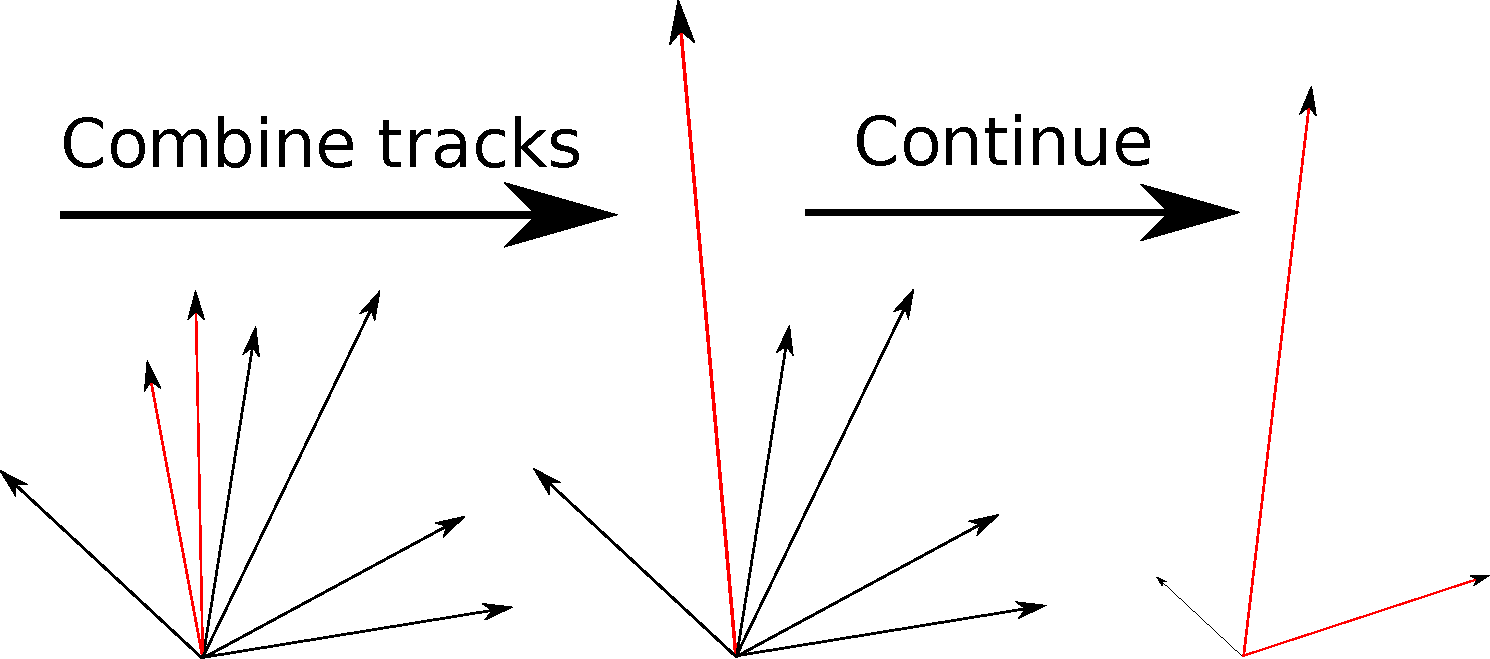
\includegraphics[width=0.8\textwidth]{pics/ktalg.pdf}
    \caption{A simple example of the antil-$\kt{}$ algorithm in progress. The red tracks in the leftmost figure are identified to have the smallest $k_{T,i}$ in the event and are combined into the red track of the middle figure. As this continues the remaining tracks are added to this or other jets. One tracks was deemed to be isolated enough to be counted as a protojet by itself. Note that the rightmost figure is zoomed out.}
    \label{fig:ktalg}
  \end{figure}






\subsection{Definition of \texorpdfstring{$\jt{}$}{jT} }
The reconstructed jet axis is used for $\jt{}$ reference. Any charged track within a fixed cone with radius $R$ is taken as a jet constituent, as opposed to using the constituent list provided by the jet algorithm. Anti-$\kt{}$ produces jets that are very circular in shape. Thus this doesn't change the constituent list considerably. Calorimeter clusters are used only in jet reconstruction.

The jet fragmentation transverse momentum, $\vec{\jt{}}$, is defined as the component of the constituent track momentum, $\vec{p}_{\mathrm{track}}$, transverse to the jet momentum, $\vec{p}_{\mathrm{jet}}$. It represents the transverse kick with respect to the initial hard parton momentum that is given to a fragmenting particle during the fragmentation process, which is a measure of the momentum spread of the jet fragments.

   \begin{figure}
    \begin{center}
      \includegraphics[width = 0.60\textwidth]{figures/tikz/jtdef}
    \end{center}
    \caption{Illustration of $\vjt{}$. The jet fragmentation transverse momentum, $\vjt{}$, is defined as the transverse momentum component of the track momentum, $\vec{p}_{\mathrm{track}}$, with respect to the jet momentum, $\vec{p}_{\mathrm{jet}}$.}
    \label{fig:jtdefinition}
  \end{figure}

The resulting $\vjt{}$ is illustrated in~\fig{fig:jtdefinition}. The length of the $\vjt{}$ vector is

  \begin{equation}
    \jt{} = \frac{|\vec{p}_{\mathrm{jet}} \times \vec{p}_{\mathrm{track}}|}{|\vec{p}_{\mathrm{jet}}|} \,.
  \label{eq:jtdefinition}
  \end{equation}


 
 
Resulting $\jt{}$ distributions are shown as 
\begin{equation}
\frac{1}{\jt{}}\frac{\mathrm{d}N}{\mathrm{d}\jt{}}
\end{equation}
distributions. The logic behind this is that $\jt{}$ is inherently a two-dimensional observable, comprised of $\jt{x}$ and $\jt{y}$ components. So the actual physical observable would be 
 
 \begin{equation}
 \frac{\mathrm{d}^2N}{\mathrm{d} \jt{x} \mathrm{d} \jt{y}}
 \end{equation}

\noindent Changing into polar coordinates with $\jt{r} = \jt{}$ and $\theta$ gives
 \begin{equation}
 \frac{\mathrm{d}^2N}{\jt{} \mathrm{d} \jt{} \mathrm{d} \theta},
 \end{equation}

\noindent where $\jt{}$ over the azimuth $\theta$ should stay constant and it can be integrated over, which gives 
\begin{equation}
\frac{1}{2\pi}\frac{\mathrm{d}N}{\jt{} \mathrm{d} \jt{}}.
 \end{equation}
 
Results of the raw inclusive $\jt{}$ distribution in four $\pt{,jet}$ bins with background are shown in Figure~\ref{fig:inclusive}. Background, i.e. the contribution from the underlying event, is further discussed in Section~\ref{sec:bg}
 
 \begin{figure}
\centering
\begin{subfigure}{0.95\textwidth}
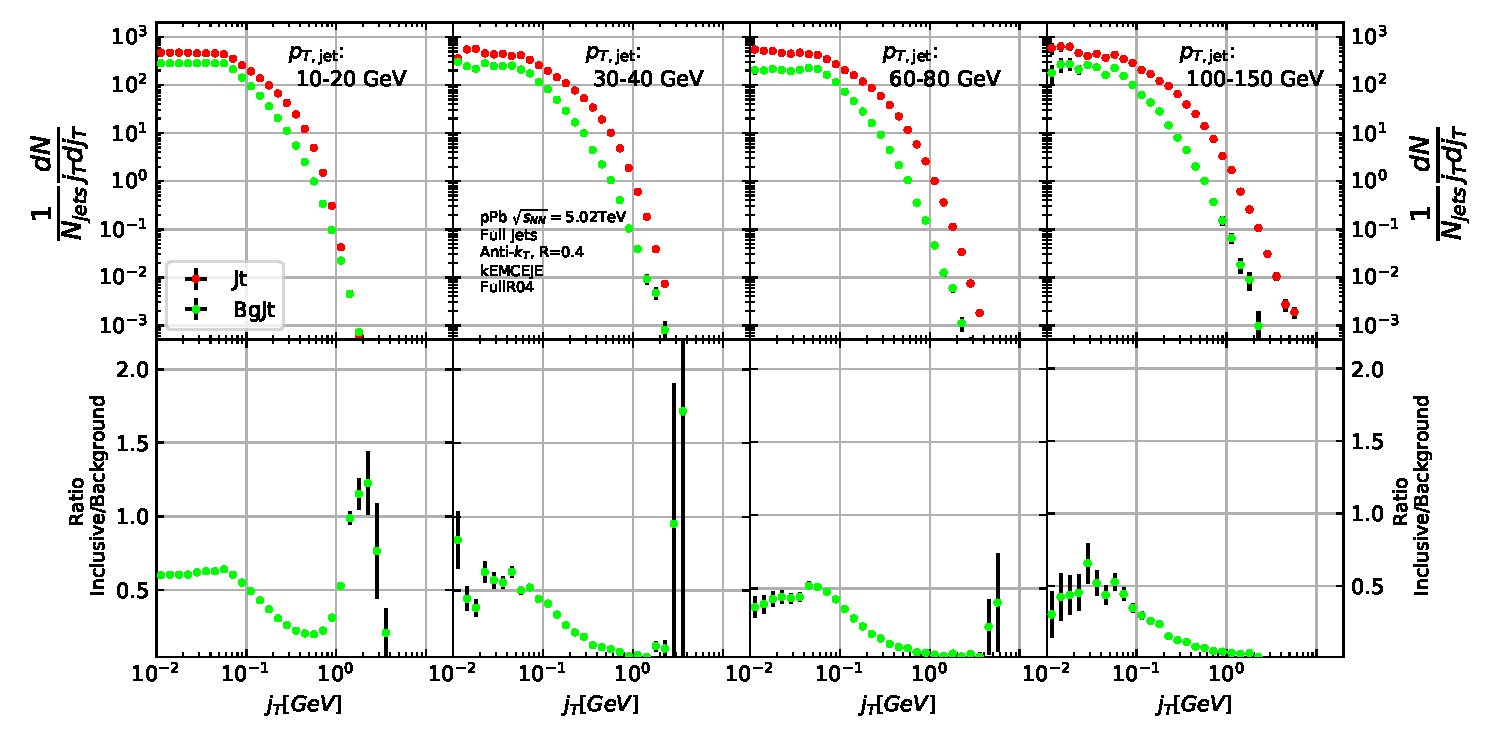
\includegraphics[width=\textwidth]{results/MixedFullJetsR04JetConeJtInclusive.pdf}
%Tag 20170810 python2.7 Python/InclusiveWithBackground.py legotrain_CF_pPb-1053_20170223-2002_LHC13bcde.root
\end{subfigure}
\caption{Inclusive $\jt{}$ with background}
\label{fig:inclusive}
\end{figure}

 
\subsection{Unfolding detector effects}
The raw inclusive $\jt{}$ distributions are corrected for the detector inefficiency with an unfolding procedure. The procedure uses response matrices obtained from a \textsc{Pythia}~\cite{introPythia81} simulation.

Measured distributions are affected by two main factors; Limited acceptance - The probability to observe a given event is less than one and limited resolution - Quantity $x$ cannot be determined exactly, but there is a measurement error. True $f(x)$ and measured $g(y)$ distributions are connected by a convolution integral. Including statistical fluctuations this becomes
\begin{equation}
\hat g(y) = \int_a^b A\left(y,x\right) f(x) dx + \epsilon(y),
\end{equation}

\noindent where A is the detector response obtained by (for example) Monte Carlo simulations and $\epsilon(y)$ is the term coming from statistical fluctuations.
If $x$ and $y$~ are discrete variables we have
\begin{equation}
\hat g_i = \sum_{j=1}^m A_{ij}f_j+\epsilon_i,
\end{equation}

where $i$ and $j$ give the $\jt{}$ bins in the true and measured distributions. $f_j$ and $g_i$ give the counts in these bins.
\noindent Or in matrix form
\begin{equation}
\hat g = Af+\epsilon,
\end{equation}
\noindent where $\hat g$ and $f$ are vectors corresponding to the measured and true histograms. If the only detector effect is limited acceptance, $A$ is a diagonal matrix, i.e. $A_{ij}=0$ for $i\neq j$. We want to deduce the true distribution $f$, when the measured distribution $g$ is known. In a general discrete case the (naive) solution is obtained by the inverse matrix
\begin{equation}
\hat f = A^{-1}\hat g 
\end{equation}
However this usually leads to oscillating solutions and determining the inverse matrix can be difficult.

Two common methods to perform this inversion are Bayesian and SVD unfolding methods. Often the solution requires some additional {\emph{ a priori}} information. For example the solution should be smooth in most cases.

\subsubsection{Bayesian unfolding}
The bayesian (iterative) method is based on the Bayes formula~\cite{ADictionaryofStatistics}.
\begin{equation}
P\left(C_i |E_j\right)=\frac{P\left(E_j |C_i\right)P_0\left(C_i\right)}{\sum_{l=1}^{n_C}P\left(E_j |C_l\right)P_0\left(C_l\right)},
\end{equation}

\noindent i.e. the probability of Cause $C_i$ ("truth") given Effect $E_j$ ("observed") is proportional to the probability of observing $E_j$ given $C_i$, $P\left(E_j |C_i\right)$ (response matrix) and the true distribution $P_0\left(C_i\right)$.

In the unfolding procedure $P_0$ is given some starting distribution, either a uniform distribution or some guess of the final distribution. Taking into account the inefficiency this gives 

\begin{equation}
\hat n\left(C_i\right) = \frac{1}{\epsilon_i} \sum_{j=1}^{n_E}n\left(E_j\right)P\left(C_i | E_j\right),
\end{equation}
%\item First calculate $P\left(C_i |E_j\right)$ with the uniform distribution
\noindent where 
\begin{equation}
P\left(C_i |E_j\right)=\frac{P\left(E_j |C_i\right)P_0\left(C_i\right)}{\sum_{l=1}^{n_C}P\left(E_j |C_l\right)P_0\left(C_l\right)},
\end{equation}


\noindent and $n\left(E_j\right)$ are the observed frequencies. First  $P\left(C_i |E_j\right)$ is calculated with the uniform distribution or best guess of the shape of the distribution. This is then used to calculate the new distribution $\hat P\left(C_i\right)$
\begin{equation}
\hat N_{true} = \sum_{i=1}^{n_C} \hat n\left(C_i\right),\,\hat P\left(C_i\right) = P\left(C_i | n\left(E\right)\right) = \frac{\hat n\left(C_i\right)}{\hat N_{true}}
\label{eq:unfolded}
\end{equation}

$P_0$ is then replaced with $\hat P$ and the procedure is repeated until an acceptable solution is found. One way to gauge the acceptability is measuring the change between iterations. Initially there is a large change between iterations, but it should get small when close to the final distribution. The number of iterations should be as low as possible, as the errors increase when going further in the iterations, but the number of iterations must be high enough so that the correct distribution is extracted. 

The bayesian procedure alongside with the SVD unfolding method are implemented in the RooUnfold package~\cite{roounfold}, which is used to perform the unfolding in practice. SVD unfolding is another procedure that utilises the Singular Value Decomposition (SVD) of the response matrix to find the inverse of the response matrix~\cite{Hocker:1995kb}.
 
 \subsubsection*{Error propagation in the Bayesian procedure }
 The measured distribution has some statistical uncertainty, this should be reflected in the unfolded distribution. Additionally the response matrix may have some uncertainty if the statistics used in the Monte Carlo simulation were limited. 
 
For errors originating from the measured distribution RooUnfold uses the error propagation matrix 

\begin{equation}
\frac{\partial \hat n\left(C_i\right)}{\partial n\left(E_j\right)} = M_{ij} + \frac{\hat n\left(C_i\right)}{n_0\left(C_i\right)}\frac{\partial n_0\left(C_i\right) }{\partial n\left(E_j\right) } - \sum_{k=1}^{n_E}\sum_{l=1}^{n_C} \frac{n\left(E_k\right) \epsilon_l}{n_0\left(C_l\right)} M_{ik} M_{lk} \frac{\partial n_0 \left(C_l\right)}{\partial n\left(E_j\right)},
\end{equation} 
 
\noindent where $\hat n \left(C_i\right)$ is the unfolded result from Eq.~\ref{eq:unfolded}. This depends upon the matrix $\frac{\partial n_0\left(C_i\right)}{\partial n\left(E_j\right) }$, which is $\frac{\partial \hat n\left(C_i\right) }{\partial n\left(E_j\right) }$ from the previous iteration. In the first iteration, $\frac{\partial n_0\left(C_i\right) }{\partial n\left(E_j\right) }=0$ and $\frac{\partial \hat n\left(C_i\right) }{\partial n\left(E_j\right) } = M_{ij}$.
 
 The error propagation matrix $V$ is used to obtain the covariance matrix on the unfolded distribution 
 
 \begin{equation}
 V\left(\hat n\left(C_k\right), \hat n\left(C_l\right)\right) = \sum_{i,j=1}^{n_E} \frac{\partial \hat n\left(C_k\right) }{\partial n\left(E_i\right) }  V\left(\hat n\left(E_i\right), \hat n\left(E_j\right)\right)  \frac{\partial \hat n\left(C_l\right) }{\partial n\left(E_j\right) },
 \end{equation}
 
\noindent where $V\left(\hat n\left(E_i\right), \hat n\left(E_j\right)\right)$ is the covariance matrix of the measurements. In counting experiments common in particle physics, each bin is independently Poisson distributed, with
 
 \begin{equation}
 V\left(\hat n\left(E_i\right), \hat n\left(E_j\right)\right) = n\left(E_i\right) \delta_{ij}
 \end{equation}
 
 \noindent The error propagation matrix for the response matrix is 
 
 \begin{multline}
 \frac{\partial \hat n\left(C_i\right)}{\partial P \left(E_j| C_k\right)} = \frac{1}{\epsilon_i}\left(\frac{n_0 \left(C_i\right) n\left(E_j\right)}{f_j} - \hat n \left(C_i\right) \right) \delta_{ik} - \frac{n_0 \left(C_k\right) n\left(E_j\right)}{f_j} M_{ij} + \\
  \frac{\hat n\left(C_i\right)}{n_0\left(C_i\right)} \frac{\partial n_0\left(C_i\right)}{\partial P \left(E_j| C_k\right)} - \frac{\epsilon_i}{n_0\left(C_i\right)} \sum_{l=1}^{n_E}\sum_{r=1}^{n_C} n\left(E_l\right) M_{il} M_{rl} \frac{\partial n_0 \left(C_r \right)}{\partial P \left(E_j| C_k\right)},
 \label{eq:responseerror}
 \end{multline}
 
\noindent where $ \frac{\partial n_0\left(C_i\right)}{\partial P \left(E_j| C_k\right)}$ is the error propagation matrix from the previous iteration, $\frac{\hat n\left(C_i\right)}{\partial P \left(E_j| C_k\right)}$. For the first iteration, this is zero and the final two terms in Eq.~\ref{eq:responseerror} disappear.
 
 The covariance matrix due to these errors is given by
 
 \begin{equation}
 V\left(\hat n\left(C_k\right), \hat n\left(C_l\right)\right) = \sum_{j,s=1}^{n_E} \sum_{i,r=1}^{n_C} \frac{\partial \hat n\left(C_k\right) }{\partial P\left(E_j | C_i\right) }  V\left(P\left(E_j | C_i\right), P\left(E_s | C_r\right) \right)  \frac{\partial \hat n\left(C_l\right) }{\partial P\left(E_s | C_r\right) },
 \end{equation}
 
\noindent where $V\left(P\left(E_j | C_i\right), P\left(E_s | C_r\right) \right)$ can be taken as multinomial, Poisson or other distribution.
 
\subsubsection{Toy Monte Carlo} 
 A toy Monte Carlo simulation was performed to see the performance of unfolding in an ideal case.
The simulations samples jet $\pt{}$ values from the observed $\pt{}$ distribution. Starting from this $\pt{}$ the simulations starts creating tracks with 
\begin{equation}
p_{\mathrm{track}} = z_\mathrm{track} \pt{,jet}
\end{equation}

\noindent where $z_\mathrm{track} $ is sampled from the observed $z$ distribution. Tracks are given random $\eta$ and $\phi$ values from uniform distributions centred at 0. All tracks below \unit[0.15]{\gev} are discarded. Sampling is continued until the sum of the track transverse momenta exceeds the jet transverse momentum. The sum of all the track momenta is calculate. This is sum is then defined to be the jet.

Simultaneously a $\pt{}$ dependant observation efficiency is applied to the tracks and a separate observed jet is calculated using only the observed tracks. Additionally a set of fake tracks is added to the observed jet. Fake tracks are generated identically to normal tracks, except for \pt{,track}, which is taken from an uniform distribution between \unit[0.15]{\gev} and \unit[1]{\gev}. Tracks are always either observed or not at the true momentum. No smearing is added to the observed momentum.

Afterwards the tracks are looped over for $\jt{}$ calculation. For observed tracks we calculate $\jt{}$ with respect to both the true jet axis and the observed jet. 2D Response matrix is filled with \begin{equation}
\left(\jt{}^\mathrm{obs},\pt{,jet}^\mathrm{obs}, \jt{}^\mathrm{true},\pt{,jet}^\mathrm{true}\right)
\end{equation}

In practice this is done with a set of 3D histograms, where \pt{jet,true} determines the histogram index and the remaining three values the bin in the 3D histogram.

After creating the response matrices, an identical procedure is carried out to the create testing data. Now instead of filling response matrices, 2D histograms are filled with $\left(\jt{}^\mathrm{obs},\pt{,jet}^\mathrm{obs}\right)$ and $\left(\jt{}^\mathrm{true},\pt{,jet}^\mathrm{true}\right)$

The observed distributions are unfolded using the 2D Bayesian (iterative) algorithm of RooUnfold. Results are shown in Figure~\ref{fig:toymc}. Aside from some discrepancy at very low \jt{} the true distribution is retrieved well. 

\begin{figure}
\centering
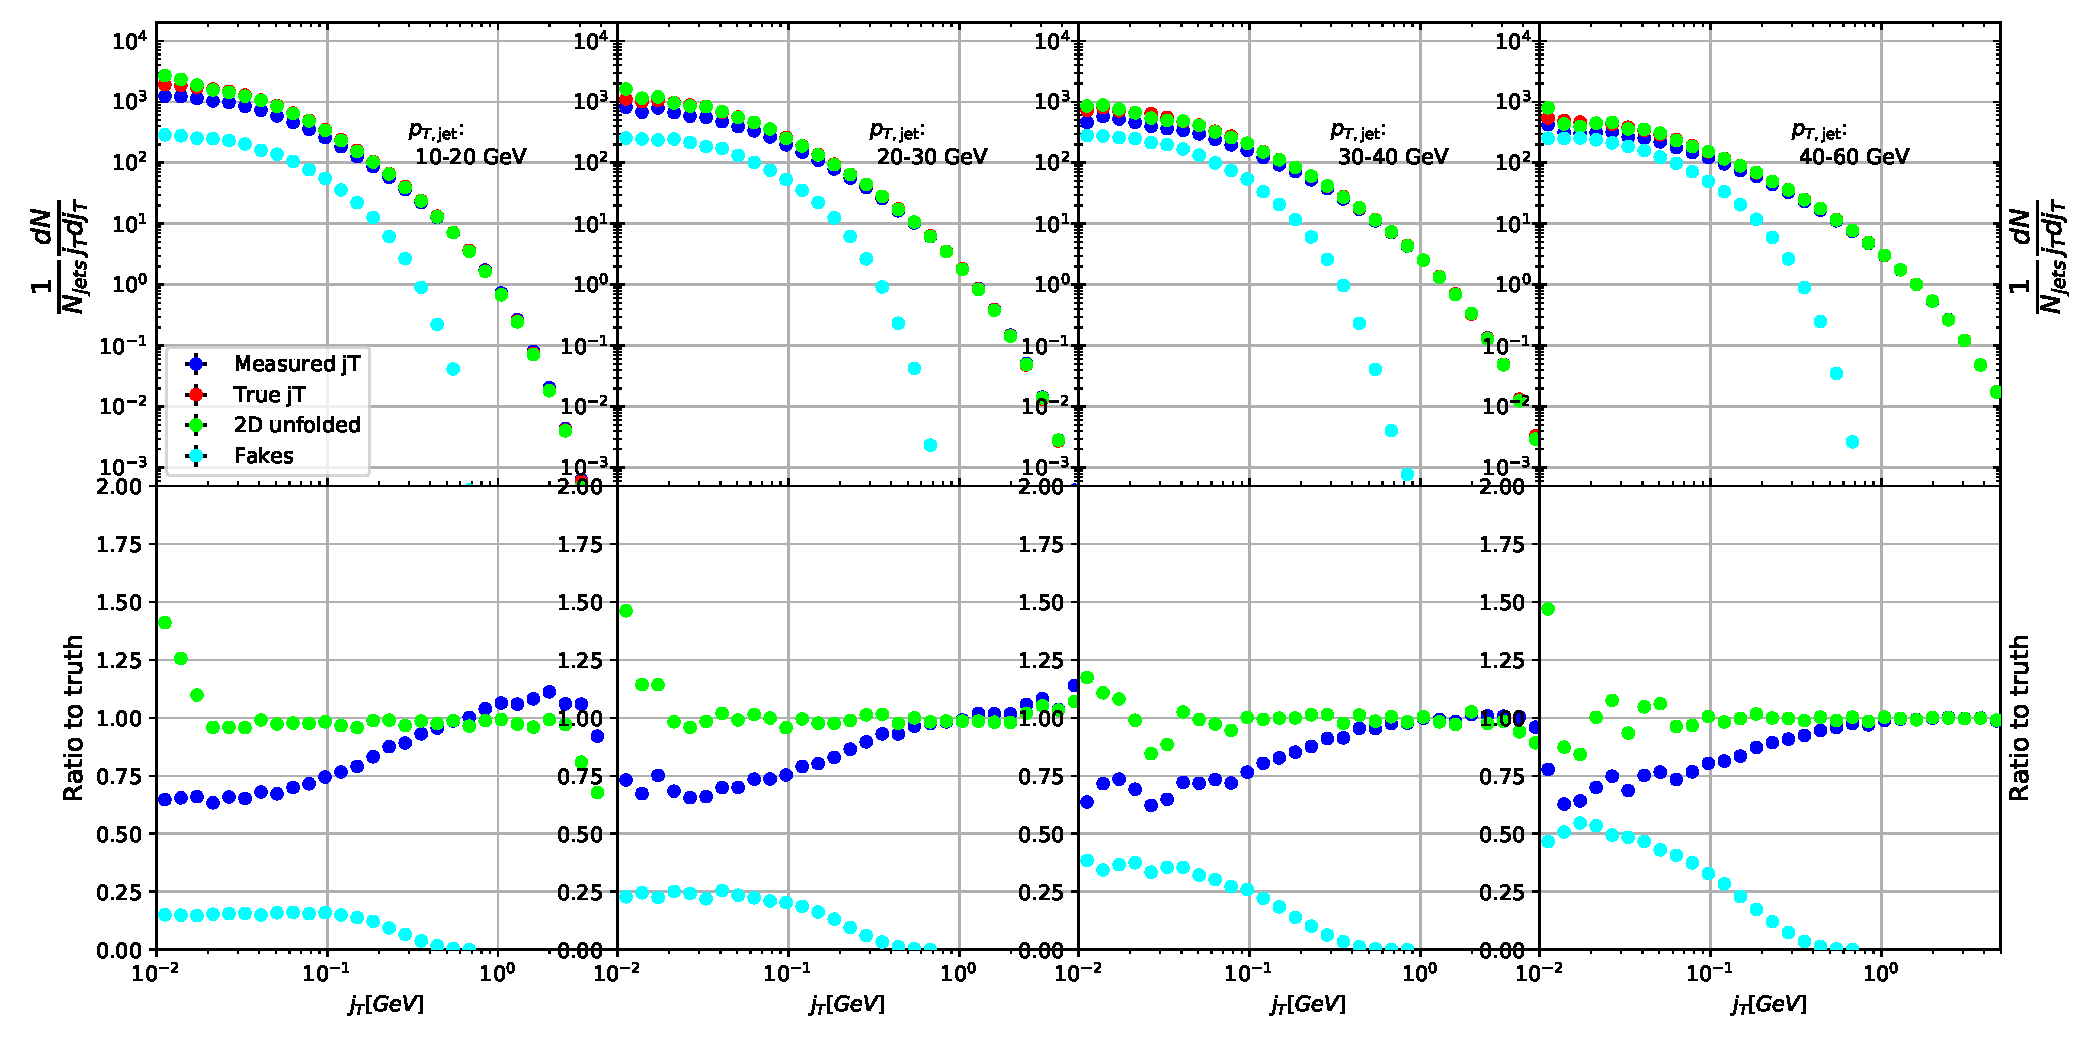
\includegraphics[width=0.9\textwidth]{figures/analysis/ToyMCUnfolder_300k_events.pdf}
\caption{Results from unfolding in Toy Monte Carlo}
\label{fig:toymc}
\end{figure}
\FloatBarrier






\subsubsection{Pythia Response matrices}
A \pythia~6 simulation was carried out to determine the response matrices.  The simulation used the Perugia 2011~\cite{pythiaPerugiaTune} tune with \snn=5.02\tev. The detector response of the particle level tracks was simulated using GEANT3~\cite{Brun:118715,geant}.

Response matrices are filled through correlation between MC detector and particle level jets and tracks. When creating the response matrices detector level tracks in each event are first analysed using the same procedure as for data, but their $\jt{}$ values are stored in an array. This is only done for tracks that are closer than the cone size, $R$, to a jet. Thus most tracks in the event will not have their $\jt{}$ values calculated. The analysis then moves to particle level (MC) tracks. There are analysed similarly, but for each track the code checks whether a corresponding detector level track existed and if that track had a \jt{} value. Finally the code checks for detector level tracks that don't have corresponding particle level track with a \jt{} value.

There are several possibilities that have to be taken into account:
\begin{itemize}
\item We find a corresponding track with a \jt{} value. Response matrix is filled normally with $\left(\jt{}^\mathrm{obs},\pt{,jet}^{obs},\jt{}^\mathrm{true},\pt{,jet}^{true}\right)$
\item We don't find a corresponding track. Record $\left(\jt{}^\mathrm{true},\pt{,jet}^\mathrm{true}\right)$ as a miss 
\item We find a corresponding track, but it didn't have $\jt{}$ value. Most likely because it was not part of a jet in the detector level set. Similary record $\left(\jt{}^\mathrm{true},\pt{,jet}^\mathrm{true}\right)$ as a miss
\item For detector level tracks that have no correspondence in particle level set the code records  $\left(\jt{}^\mathrm{obs},\pt{,jet}^\mathrm{obs}\right)$ as a fake
\end{itemize}

In the analysis code the response matrix is made of an array of 3 dimensional histograms, with $\left(\jt{}^\mathrm{obs},\pt{,jet}^\mathrm{obs},\jt{}^\mathrm{true}\right)$ as axes. The histogram index gives the $\pt{,jet}^\mathrm{true}$ value. The ranges in the response matrices of both $\jt{}$ and $\pt{,jet}$ match the ranges used for the end results. For \jt{} the range is between \unit[0.01]{\gev} and \unit[20]{\gev} and \pt{,jet} between \unit[5]{\gev} and \unit[500]{\gev}.  The ranges are the same in detector and particle level.

As a primary method unfolding is performed with an iterative (bayesian) algorithm using the RooUnfold~\cite{roounfold} package. The number of iterations used is 4.  As a default the true $\jt{}$ distribution from the \pythia~simulation is used as the prior.

%\begin{table}
%\centering
%\caption{$\jt{}$ and $\pt{}$ ranges used in unfolding. The same ranges are used for detector and truth level.}
%\label{tab:unfranges}
%\begin{tabular}{c | c | c}
% & $\jt{}$ & $\pt{,jet}$ \\
% \hline
%Min & 0.01 & 5 \\
%Max & 20 & 500 \\
%\hline
%\end{tabular}
%\end{table}

\subsubsection{Unfolding  closure test}
The \pythia~set is divided into 2 halves. First is used to fill the response matrices, as well as record missed and fake tracks. Second half is used to test the effectiveness of the unfolding method. Jet $\pt{}$ distributions and response matrix are shown in Figure~\ref{fig:ptclosure}. For the range where this analysis is performed, $\unit[40]{\gev} <\pt{,jet} <\unit[150]{\gev}$, the \pt{,jet} distribution is recovered well. At low \pt{,jet} the true distribution can't be recovered. The primary reason is that jet with $\pt{,obs}<\unit[5]{\gev}$ are not considered, although $\pt{,true}$ would have been above $\unit[5]{\gev}$. Thus these are missing from the response matrix and their contribution can't be unfolded. At high $\pt{,jet}$ the situation is opposite. Jets with $\pt{,true} > \unit[500]{\gev}$ are lost due to histogram limits. Thus jets just below this limit are overrepresented in the response matrix for $\pt{,obs}\approx \unit[500]{\gev}$. 
 
 \begin{figure}
\begin{subfigure}[b]{0.5\textwidth}
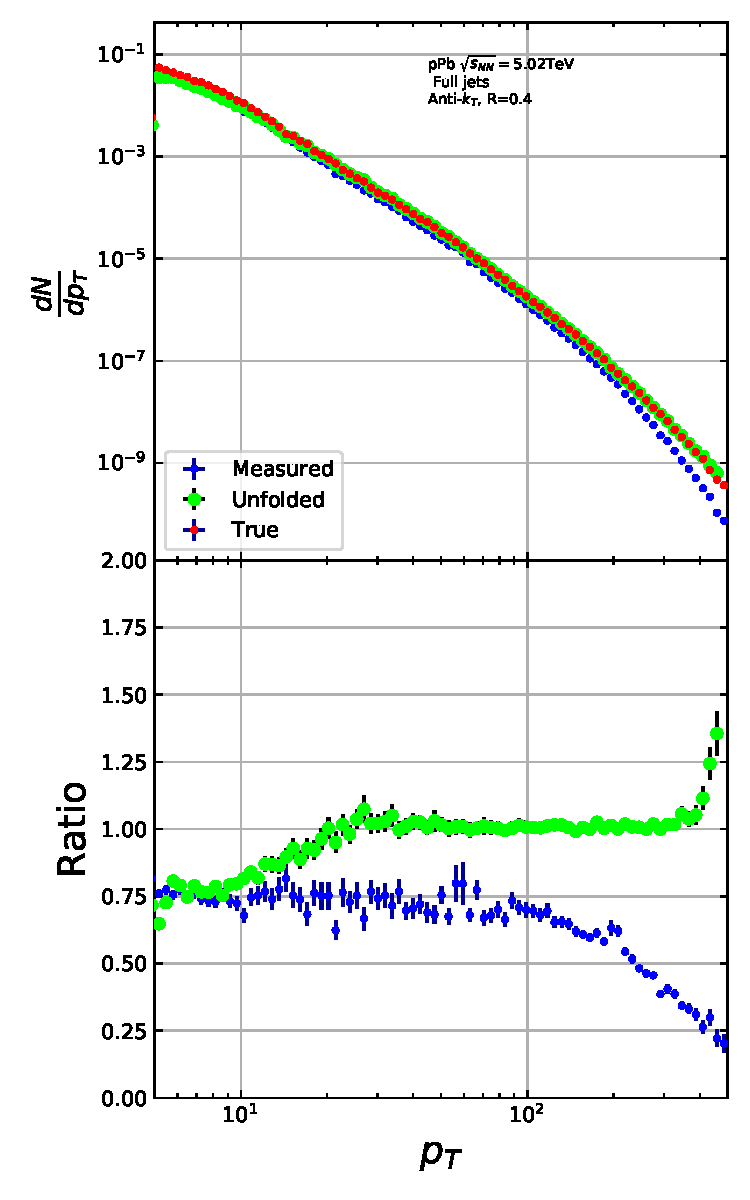
\includegraphics[width=0.7\textwidth]{figures/analysis/JetPtUnfolded.pdf}
%\caption{Unfolded jet $\pt{}$ distribution in \pythia~closure test}
%\label{fig:jetptunf}
\end{subfigure}
\begin{subfigure}[b]{0.5\textwidth}
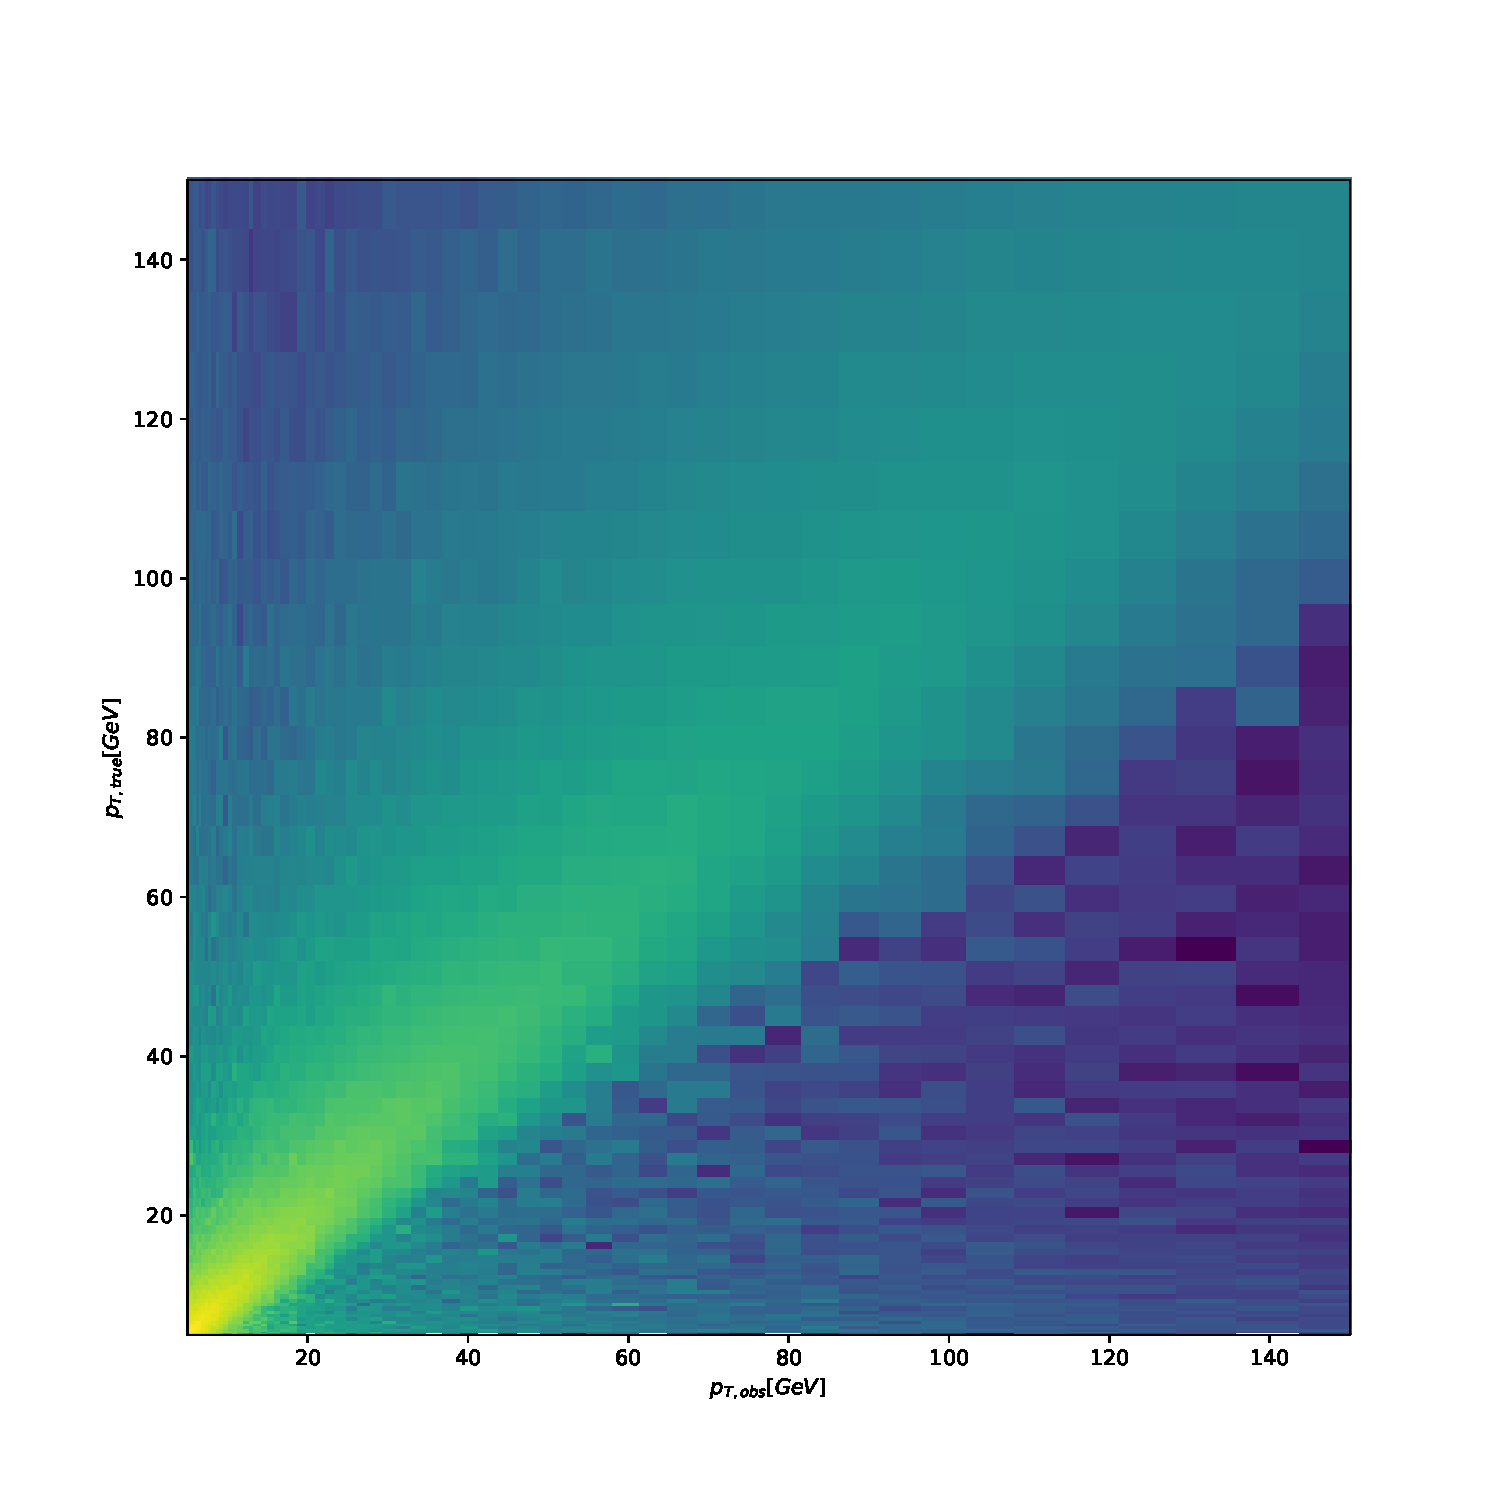
\includegraphics[width=0.8\textwidth]{figures/analysis/JetPtResponse.pdf} 
%\caption{Jet $\pt{}$ response matrix from unfolding closure test}
%\label{fig:jetptresponse}
\end{subfigure}
\caption{\emph{left:} Unfolded jet $\pt{}$ distribution in \pythia~closure test \emph{right:} Jet $\pt{}$ response matrix from unfolding closure test}
\label{fig:jetptclosure}
\end{figure}
 
Response matrices within single jet $\pt{}$ bins are shown in Figure~\ref{fig:response}. Results from the closure test are shown in Figure~\ref{fig:closure}. In the lowest jet $\pt{}$ bins unfolding fails to recover the true distribution. The lowest jet $\pt{}$ bins are dominated by combinatorial jets and thus the true detector response is likely not retrieved.

Above $\unit[30]{\gev} <\pt{,jet} < \unit[40]{\gev}$~the distribution is recovered well in the mid $\jt{}$ region. At $\jt{} < \unit[0.1]{\gev}$ there is clear discrepancy and hence the final results are shown only for $\jt{} > \unit[0.1]{\gev}$. Additionally there is some discrepancy at very high $\jt{}$. This is taken into account in the unfolding systematics. %{\color{red}(TODO: Show this) }
\begin{figure}
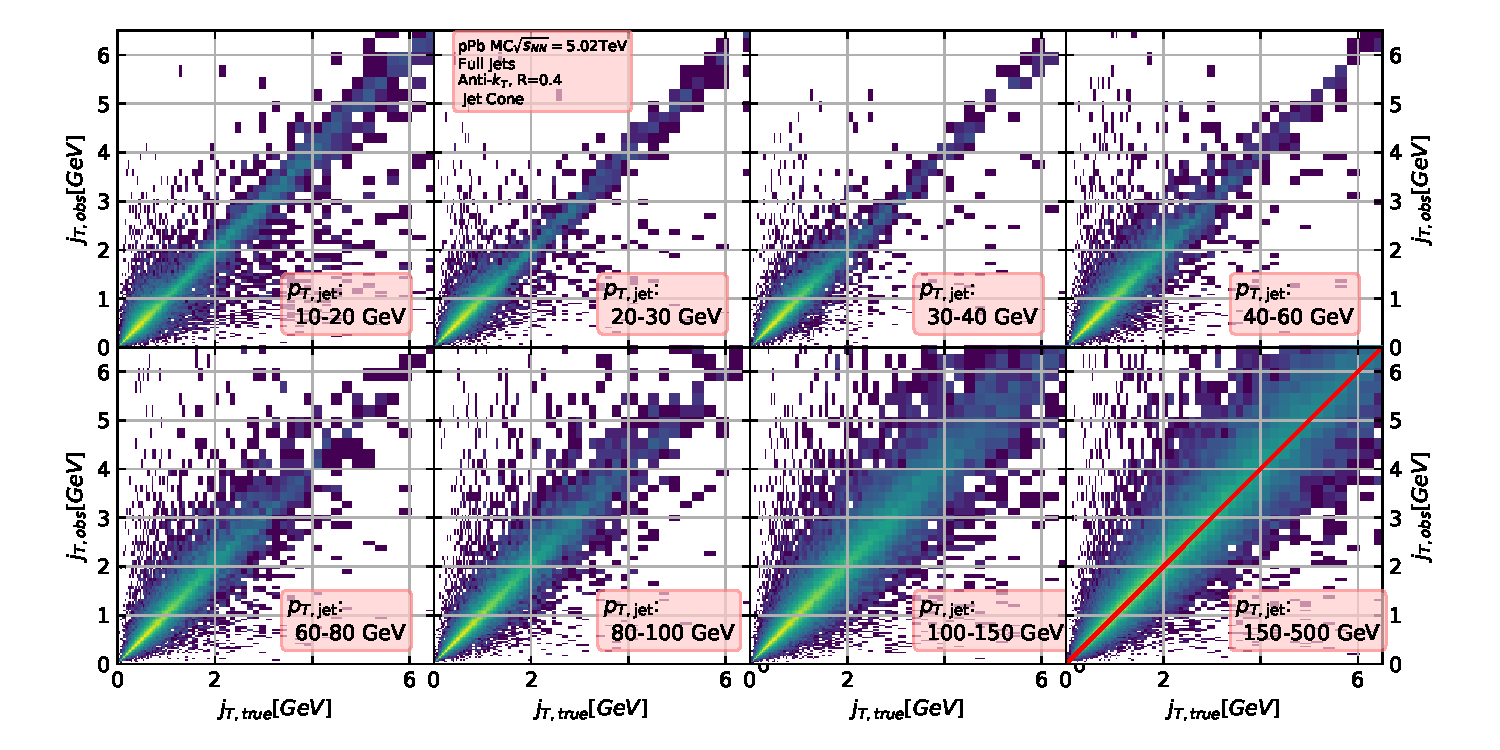
\includegraphics[width=0.99\textwidth]{figures/analysis/ResponseMatrixNFin00.pdf}
\caption{$\jt{}$ Response matrices in individual $\pt{,jet}$ bins}
\label{fig:response}
\end{figure}

\begin{figure}
\includegraphics[width=0.99\textwidth]{figures/analysis/PythiaTest.pdf}
\includegraphics[width=0.99\textwidth]{figures/analysis/PythiaTest_Extra.pdf}
\caption{Pythia closure test results. Fake tracks include also tracks that do exist in the true dataset, but for one reason or another were not given $\jt{}$ values. $\jt{}$ is only calculated for tracks that are associated with jets.}
\label{fig:closure}
\end{figure}


\FloatBarrier


 
\subsection{Background}
\label{sec:bg}
When calculating \jt{} distributions for jet constituents there is a contribution from the underlying event (UE), i.e. tracks that just happen to be close to the jet axis.
To find the signal coming from the actual jet we need to subtract the background (UE) contribution. On a jet-by-jet basis this is difficult to achieve reliably, so one must estimate the background contribution in the inclusive  distribution. A schematic view of the background contribution is shown in Figure~\ref{fig:bgdef}. 

We have two methods for background estimation. In the first we look at the direction perpendicular to the jet. This is assumed to be the region least likely to contain jet contributions. In the second method we randomly assign the tracks of event new $\phi$ and $\eta$ values. The result is thus guaranteed to be uncorrelated.

\begin{figure}[h]
\centering
\begin{subfigure}{0.4\textwidth}
\begin{tikzpicture}
\draw[gray, thick, ->] (0,0) -- (1,2);
\draw[gray, thick, ->] (0,0) -- (-0.8,2.2);
\draw[gray, thick, ->] (0,0) -- (-0.1,1.5);
\draw[gray, thick, ->] (0,0) -- (0.7,1.7);
\draw[green, thick] (0,0) -- node[near end, right] {Jet cone}(1.5,2.8);
\draw[green, thin, <->] (0,2.8) -- node[midway, above] {$R$} (1.5,2.8);
\draw[green, thick] (0,0) --  (-1.5,2.8);
\draw[blue, thin, ->] (0,2.2) -- node [midway, above] {\jt{}} (-0.8,2.2);
\draw[black, very thick, ->] (0,0) -- node [near end,right] {jet} (0,3);
\draw[black, very thick, ->] (0,0) -- node [near end, right] {Awayside jet?} (0,-2);
\draw[red, thin, ->] (0,0) -- (-1.25982281336992,-1.55333398820495);
\draw[red, thin, ->] (0,0) -- (-1.45147226001971,0.514614689251372);
\draw[red, thin, ->] (0,0) -- (-0.30285006631157,-1.69312782663775);
\draw[red, thin, ->] (0,0) -- (0.8074529522207,0.832838357636147);
\draw[red, thin, ->] (0,0) -- (-1.48782136581293,-0.397476519344932);
\draw[red, thin, ->] (0,0) -- (0.935437036685518,-1.76775494636474);
\draw[red, thin, ->] (0,0) -- (-0.905166754522554,1.2459025429411);
\draw[red, thin, ->] (0,0) -- (0.392170769946368,1.89994791697027);
\draw[red, thin, ->] (0,1.89994791697027) -- node [near start, left] {\jt{}} (0.392170769946368,1.89994791697027);
\end{tikzpicture}

\caption{Orange is underlying event while gray tracks represent the signal}
\end{subfigure}
\begin{subfigure}{0.4\textwidth}
\documentclass[border=5mm]{standalone}
\usepackage{tikz}
\usetikzlibrary{positioning}
\usepackage{xcolor}
\usetikzlibrary{shapes,arrows}
\usetikzlibrary{trees}
\usetikzlibrary{shadows.blur}
\usetikzlibrary{decorations.pathmorphing}
\usetikzlibrary{decorations.markings}
\usetikzlibrary{intersections, calc}
\def\jt#1{\ensuremath{j_{\rm T#1}}}
\begin{document}
\begin{tikzpicture}
\draw[gray, thick, ->] (0,0) -- (1,2);
\draw[gray, thick, ->] (0,0) -- (-0.8,2.2);
\draw[gray, thick, ->] (0,0) -- (-0.1,1.5);
\draw[gray, thick, ->] (0,0) -- (0.7,1.7);
\draw[blue, thick] (0,0) -- (-2.8,1.5);
\draw[blue, thick] (0,0) --  (-2.8,-1.5);
\draw[blue, very thick, ->] (0,0) -- node [near end, above] {Rotated axis} (-3,0);
\draw[black, very thick, ->] (0,0) -- node [near end,right] {jet} (0,3);
\draw[black, very thick, ->] (0,0) -- node [near end, right] {Awayside jet?} (0,-2);
\draw[orange, thin, ->] (0,0) -- (-1.25982281336992,-1.55333398820495);
\draw[orange, thin, ->] (0,0) -- (-1.45147226001971,0.514614689251372);
\draw[orange, thin, ->] (0,0) -- (-0.30285006631157,-1.69312782663775);
\draw[orange, thin, ->] (0,0) -- (0.8074529522207,0.832838357636147);
\draw[orange, thin, ->] (0,0) -- (-1.48782136581293,-0.397476519344932);
\draw[orange, thin, ->] (0,0) -- (0.935437036685518,-1.76775494636474);
\draw[orange, thin, ->] (0,0) -- (-0.905166754522554,1.2459025429411);
\draw[orange, thin, ->] (0,0) -- (0.392170769946368,1.89994791697027);
\draw[orange, thin, densely dotted] (-1.48782136581293,0) -- node [midway, left] {\small bg $\jt{}$} (-1.48782136581293,-0.397476519344932);
\end{tikzpicture}
\end{document}

\caption{We estimate the background using a cone where the axis is perpendicular to the jet axis}
\end{subfigure}
\caption{Background estimation}
\label{fig:bgdef}
\end{figure}

\subsubsection{Perpendicular cone background}
As a primary method to estimate the background we look at regions of the detector where there are no tracks from jets, but only uncorrelated tracks from the underlying event. The underlying event is thus estimated by looking at an imaginary jet cone perpendicular to the observed jet axis ($\frac{\pi}{2}$ Rotation in $\phi$). 

%$\jt{}$ is calculated for any tracks found within this cone. The vector sum of the individual track momentum and the imaginary jet axis is used as reference for $\jt{}$. The background obtained in this manner is subtracted from the unfolded inclusive $\jt{}$ distribution, which gives the resulting signal distribution. To make sure there is no jet contribution in the background, any events with jets inside the perpendicular cone are not used for background estimation.

After calculating the $\jt{}$ values for tracks in the jet, we rotate the jet axis by $\frac{\pi}{2}$ in positive $\phi$ direction. We check that there are no other jets closer than $2R$ to the rotated axis. Otherwise background calculation is skipped for this jet. Probability of this happening is 1-2\% depending on the jet $\pt{}$ bin.

If we don't find other jets in the vicinity we move on to estimate the background. We find all tracks within a cone of radius $R$ around the rotated axis and calculate $\jt{}$ of these tracks with respect to the rotated axis. %Auto-correlations are discussed in Section~\ref{sec:autoC}. 

This background procedure is a part of the reason for using charged tracks inside a fixed size cone, instead of jet constituents. To be representative of the actual underlying event contribution the size and shape of the background estimation region should match the area where $\jt{}$ is calculated. The irregular shape of a jet would be hard to take into account when calculating background. Thus the regions are made to match by considering fixed size cones for $\jt{}$.






\begin{figure}[tb]
\centering
\tikzstyle{decision} = [diamond, draw, fill=blue!20, 
    text width=4.5em, text badly centered, node distance=3cm, inner sep=0pt]
\tikzstyle{block} = [rectangle, draw, fill=blue!20, 
    text width=5em, text centered, rounded corners, minimum height=4em]
\tikzstyle{line} = [draw, -latex',orange]
\tikzstyle{cloud} = [draw, ellipse,fill=red!20, node distance=3cm,
    minimum height=2em]
    
\tiny 
\begin{tikzpicture}[node distance = 1cm, auto]
    % Place nodes
    \node [block] (init) {Jet found};
    \node [block, below of=init, node distance = 2cm] (rotate) {Rotate jet axis by $\pi/2$ (positive $\phi$)};
    \node [decision, below of=rotate, node distance = 2.5cm](jets){Other jets close to the rotated axis? ($<2R$)};
    \node [block, left of=jets, node distance = 2.5cm] (discard) {Don't calculate background};
    \node [block, right of=jets, node distance = 2.5cm] (tracks) {Find tracks within cone R};
    \node [block, above of=tracks, node distance = 2cm](sum) {Calculate vector sum of track and rotated axis};
    \node [block, right of =sum, node distance = 2cm](jt) {Calculate $\jt{}$ with respect to the vector sum};
    
    % Draw edges
    \path [line] (init) -- (rotate);
    \path [line] (rotate) -- (jets);
    \path [line] (jets) -- node [near start] {yes} (discard);
    \path [line] (jets) -- node [near start] {no} (tracks);
    \path [line] (tracks) -- node [near start] {For each track} (sum);
    \path [line] (sum) -- (jt);
    \path [line] (jt) |- (tracks);
    
\end{tikzpicture}

\caption{Flowchart representation of the perpendicular cone background procedure}
\label{fig:bgflow}
\end{figure}


One additional consideration is the issue of auto-correlations as the jet axis is simply a vector sum of all its constituents. Thus having an additional track in the jet from the underlying event moves the jet axis towards this track. Since the axis is now closer to the track, it has a smaller $\jt{}$ value. Assuming a \unit[1]{\gev} background track  at the edge of a $R = 0.4$ cone the $\jt{}$ value would be \unit[0.4]{\gev}. If this is added to a  \unit[5]{\gev} jet, the $\jt{}$ value becomes \unit[0.33]{\gev} after the jet axis moves. In a \unit[50]{\gev} jet it would be \unit[0.39]{\gev}. This is a region where the inclusive $\jt{}$ distribution is dominated by background. The distribution is also steeply falling. Overestimating the background can lead to a situation where the background estimation exceeds the inclusive distribution.

%\begin{figure}[htp]
%\centering
%\begin{subfigure}{0.99\textwidth}
%\includegraphics[width=0.95\textwidth]{pics/jt_in_jet_bg}
%\caption{Illustration of the effect of a track from the underlying event in a jet and for a fixed background axis}
%\end{subfigure}
%\begin{subfigure}{0.45\textwidth}
%\includegraphics[width=0.95\textwidth]{pics/jt_correction}
%\caption{Background behavior after adding auto-correlations}
%\end{subfigure}
%\caption{Auto-correlations in background and jets}
%\end{figure}

To take this effect into account we can't use a fixed axis for background, but it has to behave like a jet would when additional tracks are added. Thus before calculating $\jt{}$ values we make a vector sum of the track and the axis used for background, which is either the perpendicular cone axis or the random axis depending on the background method. In each case the momentum of this background axis is assumed to be the same as the jet which initiated the background estimation.

In \pPb data there is on average about one underlying event track in a $R = 0.4$ cone. If there would be more, one should consider taking the vector sum of all tracks inside the cone. As there is usually only one track and if there are more it's unlikely that more than one has high momentum, taking the vector sum track-by-track should be enough.








%\begin{figure}[htp]
%\centering
%\includegraphics[width=0.75\textwidth]{pics/jt_back}\\
%\end{figure}


%\begin{figure}[htp]
%\includegraphics[width=0.85\textwidth]{pics/2014-May-16-p-pb_jt_bgsub_060-080_0005-0100} \\
%\line(1,0){250}\\
%\raggedright
%\tiny{Král, Jiří, \textit{ Intrinsic Transverse Momentum Distribution of Jet
%Constituents in P-Pb Collisions at ALICE}, Ph.D. Thesis, University of Jyväskylä, 2014}
%%\item jT distribution is constructed from charged jet constituents
%\end{figure}

\subsubsection{Random background}
In the random background method we look at all tracks in the event, except for tracks close to jets found by the jet algorithm. We randomly assign new $\eta$ and $\phi$ values to all tracks using uniform distributions with $\left|\eta\right| < 1.0$. $\pt{}$ values are kept the same. To increase statistics there is a possibility to create a number of random tracks for each actual track. In the analysis we do this 10 times for each track. Again the track $\pt{}$ value is kept the same. 

We create a random jet cone from uniform $\eta$ and $\phi$ distributions. Here $\left| \eta \right| < 0.25$. Now we calculate $\jt{}$ of the random tracks with respect to the random cone axis. As in the perpendicular cone method auto-correlations are added before calculating \jt{}.

Comparison between perpendicular cone and random background in Figure~\ref{fig:bgcomparison}. The advantage of the random background method is that the procedure can be repeated several times for each event, which allows producing additional statistics. However, it seems that, especially in the highest $\pt{,jet}$ bins there is some jet contribution left at the high end. Naturally there is no correlation between the tracks and the background axis, but if some high momentum tracks originating from jets were not subtracted and happen to hit the edge of the background cone, they can increase the high $\jt{}$ yield in the background estimation.

\begin{figure}[htb]
\centering
\begin{subfigure}{0.95\textwidth}
\includegraphics[width=\textwidth]{results/MixedFullJetsR04BackgroundComparison.pdf}
%Tag 20170810 python2.7 Python/InclusiveWithBackground.py legotrain_CF_pPb-1053_20170223-2002_LHC13bcde.root
\end{subfigure}
\caption{$\jt{}$ background with two different methods}
\label{fig:bgcomparison}
\end{figure}

We observe that the results from perpendicular cone background show no observable change between $\pt{,jet}$ bins. It is a good indication that the background is actually dominated by the underlying event over the entire $\jt{}$ region. 

Thus as a primary method of background estimation the perpendicular cone method is used. The random background method is used to estimate systematic contributions by comparing the final results obtained with this method to the results obtained from the perpendicular cone method.


\FloatBarrier
 \subsection{Fitting}
 \label{sec:fitting}
After unfolding and background subtraction the resulting signal distributions are fitted with a 2 component function shown in Eq.~\ref{eq:fit}. Gaussian distribution is used for low $\jt{}$ and an inverse gamma function is used for high $\jt{}$. The Gaussian is taken to have the center at $\jt{} = 0$. In total this gives 5 parameters. The fitting procedure was inspired by the dihadron $\jt{}$ analysis by ALICE~\cite{ALICEjt}. The complete fitting function is 

\begin{equation}
\frac{1}{N_{\mathrm{jets}}}\frac{\mathrm{d}N}{\jt{} \mathrm{d}\jt{}} = \frac{B_2}{B_1\sqrt{2\pi}}e^{-\frac{\jt{}^2}{2B_1^2}}+\frac{B_3B_5^{B_4}}{\Gamma\left(B_4\right)}\frac{e^{-\frac{B_5}{\jt{}}}}{\jt{}^{B_4+1}}.
\label{eq:fit}
\end{equation}

To achieve stable results the fitting is performed in two steps. First both components are fitted separately. Gaussian component is fitted to the low end of $\jt{}$. Inverse gamma component is fitted to $\jt{}$ above $\unit[1]{\gevc}$. After getting the results from the individual fits they are combined into a single function with initial values from the individual results and an additional fit is performed. 
%Fitting only the Gaussian component to the entire distribution produces approximately the same result as the Gaussian component in the two-component model.

After getting the fit function $\sqrt{\left<\jt{}^2\right>}$ (RMS) and yield values are extracted separately from each component. The narrow component RMS is

\begin{equation}
\sqrt{\left<\jt{}^2\right>}=\sqrt{2}B_1,
\end{equation}


\noindent and the wide component RMS value is calculated as 

\begin{equation}
\sqrt{\left<\jt{}^2\right>}=\frac{B_5}{\sqrt{\left(B_4-2\right)\left(B_4-3\right)}},
\end{equation}


\noindent where it is required that $B_4 > 3$.

The statistical errors can be calculated with the general error propagation formulas. As a result one gets errors for the narrow component RMS
\nobreak
\begin{equation}
\delta \sqrt{\left<\jt{}^2\right>} = \sqrt{2}\delta B_1
\end{equation}
\noindent and for the wide component RMS

\begin{equation}
\delta \sqrt{\left<\jt{}^2\right>} = \sqrt{ \left( \frac{\left(5-2 B_4 \right) B_5 \delta  B_4}{\left( 2\left(  B_4-2\right)\left( B_4-3\right)      \right)^{\frac{3}{2}}}\right)^2 + \left( \frac{\delta B_5}{\sqrt{\left( B_4-2\right)\left( B_4-3\right)}}      \right)^2  }.
\end{equation}

%Yield(narrow)
%$$\frac{\delta Y}{N_{\mathrm{jet}}} = \sqrt{\frac{B_2^2\delta B_1^2+B_1^2\delta B_2^2}{2\pi}}$$
% Yield(Wide)
% $$ \frac{\delta Y}{N_{\mathrm{jet}}} = \sqrt{\left(\frac{B_5\delta B_3}{B_4-1} \right)^2+ \left(\frac{B_3B_5\delta B_4}{\left(B_4-1 \right)^2} \right)^2 + \left(\frac{B_3 \delta B_5}{B_4-1}\right)^2}$$



% !TEX root = thesis.tex
\section{Systematic erros}
{\color{red} Extend Systematics}
\label{sec:systematicerrors}
The main systematic uncertainties in this analysis come from the background estimation, the unfolding procedure and uncertainty in the tracking efficiency. Tracking uncertainties are estimated from variations of the track selection cuts defined in Sec.~\ref{sec:experimentaldetails}. 

%The resulting variations in RMS are shown in Table \ref{tab:systematics}. The uncertainties from unfolding and background subtraction are of the same magnitude. 

The systematics in background estimation were studied using an alternative method to extract the background, mainly the random background method. The resulting uncertainty is below 5\% for the wide component RMS and below 9\% for the narrow component RMS. 

The systematic uncertainty that arises from the unfolding procedure is estimated by performing the unfolding with two separate methods. Data corrected by the iterative unfolding method are used as the results and the SVD unfolding method is employed to estimate the uncertainty. In a \textsc{Pythia} closure test the true distribution was in general found to be between the unfolded distributions from the iterative and SVD method. The difference between the methods when unfolding data should give a reasonable estimate of the unfolding uncertainty. The resulting uncertainty is below 8\% for both wide and narrow component RMS.



\begin{table}[htb]
\centering
\caption{Summary of systematic errors}
\label{tab:systematics}
\begin{tabular}{ l | c | r }
  Systematic & Wide RMS & Narrow RMS \\
    \hline			
  Background & 5 \% & 9 \% \\
  Unfolding & 8 \% & 8 \% \\
  Tracking & ? \% & ? \% \\
  Total & 9 \% & 12\% \\
  \hline
  \end{tabular}
  \end{table}
  
 \subsection{Background}
The uncertainty coming from background estimation is estimated by subtracting the background separately for the perpendicular cone and random background methods. Comparisons of the resulting signal distributions are shown in Fig.~\ref{fig:signal}. 
 
 \begin{figure}[htb]
\centering
\begin{subfigure}{0.95\textwidth}
\includegraphics[width=\textwidth]{results/MixedFullJetsR04JetConeJtSignal.pdf}
%Tag 20170810 python2.7 Python/DrawSignal.py legotrain_CF_pPb-1053_20170223-2002_LHC13bcde.root
\end{subfigure}
\caption{$\jt{}$ signal with background subtracted}
\label{fig:signal}
\end{figure}

 
Fits are then performed on both perpendicular cone and random background signals. Difference between them is taken as the systematic error. The fits for individual bins from the random background method are shown in figure \ref{fig:fitsrandombg}. Resulting differences between the methods for different components are shown in figure \ref{fig:systbg}. The dotted lines are put at $\pm \unit[5]{\%}$ for the narrow component and at $\pm \unit[8]{\%}$ for the wide component. These are taken as systematic estimates for the entire $\pt{jet}$ range.

\begin{figure}[htb]
\centering
\begin{subfigure}{0.95\textwidth}
\includegraphics[width=\textwidth]{results/MixedFullJetsR04SignalBackgroundComparison.pdf}
%Tag 20170810 python2.7 Python/DrawSignal.py legotrain_CF_pPb-1053_20170223-2002_LHC13bcde.root
\end{subfigure}
\caption{Comparison of the effect of background method on $\jt{}$ signal.}
\label{fig:signalbg}
\end{figure}


\begin{figure}
\centering
\begin{subfigure}{0.24\textwidth}
\includegraphics[width=0.95\textwidth]{results/JetConejTSignalFit/JetConejTSignalFitNFin00JetPt04randomBgBayes}
\end{subfigure}
\begin{subfigure}{0.24\textwidth}
\includegraphics[width=0.95\textwidth]{results/JetConejTSignalFit/JetConejTSignalFitNFin00JetPt05randomBgBayes}
\end{subfigure}
\begin{subfigure}{0.24\textwidth}
\includegraphics[width=0.95\textwidth]{results/JetConejTSignalFit/JetConejTSignalFitNFin00JetPt06randomBgBayes}
\end{subfigure}
\begin{subfigure}{0.24\textwidth}
\includegraphics[width=0.95\textwidth]{results/JetConejTSignalFit/JetConejTSignalFitNFin00JetPt07randomBgBayes}
\end{subfigure}
\caption{$\jt{}$ signal with random bacgkround subtraction fits in different jet $\pt{}$ bins}
\label{fig:fitsrandombg}
\end{figure}

\begin{figure}
\centering
\begin{subfigure}{0.24\textwidth}
\includegraphics[width=0.95\textwidth]{results/SystematicErrors/SystematicErrorsGammaRMS_BgNFin00JetPt08_linx_data}
\end{subfigure}
\begin{subfigure}{0.24\textwidth}
\includegraphics[width=0.95\textwidth]{results/SystematicErrors/SystematicErrorsGausRMS_BgNFin00JetPt08_linx_data}
\end{subfigure}
\caption{Differences between perpendicular cone and random background subtraction in the resulting RMS values.}
\label{fig:systbg}
\end{figure}

  
  
  
  \subsection{Unfolding}
Unfolding is the second major source of systematic uncertainty. To estimate the uncertainty related to the unfolding procedure several checks are performed. The main systematic uncertainty estimation comes from comparing results performed using both SVD and Bayesian unfolding. Difference between the methods is taken as the systematic error. Since SVD unfolding does not have a 2 dimensional options, the unfolding is done bin by bin. The resulting distributions after SVD unfolding and background subtraction with the perpendicular cone method are shown in fig \ref{fig:fitsSVD}. 

As in the background systematic estimation, fits are performed for both cases separately. Resulting differences between the methods for different components are shown in figure \ref{fig:systunf}. The dotted lines are at $\pm \unit[8]{\%}$ for both components. These are taken to be the systematic uncertainty related to unfolding. 

\begin{figure}
\centering
\caption{Resulting signal distributions from SVD unfolding with the perpendicular cone background methods. These are compared to the results from the Bayesian algorithm to estimate the systematic uncertainty.}
\label{fig:fitsSVD}
\end{figure}
\begin{figure}
\centering
\begin{subfigure}{0.24\textwidth}
\includegraphics[width=0.95\textwidth]{results/SystematicErrors/SystematicErrorsGammaRMS_UnfNFin00JetPt08_linx_data}
\end{subfigure}
\begin{subfigure}{0.24\textwidth}
\includegraphics[width=0.95\textwidth]{results/SystematicErrors/SystematicErrorsGausRMS_UnfNFin00JetPt08_linx_data}
\end{subfigure}
\caption{Differences between Bayesian and SVD unfolding in the resulting RMS values}
\label{fig:systunf}
\end{figure}

Several other systematic checks were performed with the Bayesian unfolding procedure. They are described in the following sections. As these are small compared to the main uncertainty they are not included separately.
 
  
\subsubsection{Effect of number of iterations}
\label{sec:iterations}
The iterative unfolding algorithm permits the change of number of iterations. The unfolding procedure was carried out using different numbers of iterations. The results from these different cases are shown in Fig.~\ref{fig:iterations}. The results are compared to the default unfolding algorithm with 4 iterations. The difference in results between the different cases is mostly less than 2.5\%.
\begin{figure}
\includegraphics[width=0.99\textwidth]{figures/systematics/IterationsComparison.pdf}
\caption{Unfolding with different number of iterations}
\label{fig:iterations}
\end{figure}

\subsubsection{Effect of different prior}
\label{sec:prior}
The iterative algorithm requires a prior estimate of the shape of the distribution. As a default prior the truth (particle level) distribution is used. To test the effect of changing the prior we instead use the unfolded $\jt{}$ distribution as prior. The results are compared to the unfolding algorithm with the default prior. This is shown in Fig.~\ref{fig:prior} The difference in results between the different cases is mostly less than 2.5\%. 

\begin{figure}
\includegraphics[width=0.99\textwidth]{figures/systematics/PtCutComparison10.pdf}
\caption{Effect of changing minimum jet $\pt{}$ used in unfolding from 5 to 10 \gev. {\color{red} Wrong figure}}
\label{fig:prior}
\end{figure}

\subsubsection{Effect of $\pt{}$ truncation}
\label{sec:truncation}
As an additional check the unfolding is carried out with different $\pt{jet}$ truncation values. By default the full range of $\pt{jet} > 5 \gev$ is used. We test the unfolding by only using the response matrix for $\pt{jet} > \unit[10]{\gev}$. The results of this test are shown in Fig.~\ref{fig:truncation}. The effects are strongest in the lower $\pt{jet}$ bins. Also in this case the difference is less than \unit[2.5]{\%} in all $\pt{jet}$ bins.

\begin{figure}
\includegraphics[width=0.99\textwidth]{figures/systematics/PtCutComparison10.pdf}
\caption{Effect of changing minimum jet $\pt{}$ used in unfolding from 5 to 10 \gev}
\label{fig:truncation}
\end{figure}

\subsection{Tracking}
Systematic effects originating from uncertainty in the tracking efficiency are estimated through a \pythia~simulation, where an artificial inefficiency of 3\% is introduced i.e. 3 \% of tracks are randomly removed from each event. The effect of this artificial inefficiency is shown in Fig.~\ref{fig:trackingsyst}. The systematic uncertainties assigned to tracking efficiency are \unit[4]{\%} for the narrow component and \unit[5]{\%} for the wide component. 

\begin{figure}
\centering
\begin{subfigure}{0.45\textwidth}
\includegraphics[width=0.95\textwidth]{figures/systematics/SystematicErrorsGausRMS_Tracking.pdf}
\end{subfigure}
\begin{subfigure}{0.45\textwidth}
\includegraphics[width=0.95\textwidth]{figures/systematics/SystematicErrorsGammaRMS_Tracking.pdf}
\end{subfigure}
\caption{Relative systematic errors resulting from tracking efficiency uncertainty.}
\label{fig:systtrack2}
\end{figure}

\subsection{EMCal clusters}
The analysis uses EMCal clusters only in the reconstruction of jets. Thus the only way uncertainty in EMCal performance can affect the results is through modification of jet momentum or axis.
  
Uncertainty related to the EMCal energy scale was estimated by scaling cluster energies up and down by 2 \% in a PYTHIA particle level simulation. Similarly the jet momentum was scaled by $\pm 2\%$ when determining the jet $\pt{}$ bin. In the analysis EMCal is used only in jet reconstruction, not for calculating $\jt{}$. The only ways EMCal uncertainty can affect the analysis are changes in jet energy and jet axis. Jet axis shouldn't significantly change, so the main contribution should be changes in jet $\pt{}$ bin.

The resulting differences in the inclusive $\jt{}$ distributions are shown in Fig.~\ref{fig:systemcal}. Qualitatively the effect of scaling cluster energies is the same as scaling the jet energies.

Like in the previous cases fits are performed for the unscaled case and for cases with $\pm \unit[2]{\%}$ scaling. The resulting systematic uncertainties are shown in Fig.~\ref{fig:systemcal2}. The uncertainty is taken to be 1\% for both components.

\begin{figure}
\centering
\begin{subfigure}{0.90\textwidth}
\includegraphics[width=0.95\textwidth]{figures/systematics/HadCorrComparisonJetPt4To8.pdf}
\end{subfigure}
%\begin{subfigure}{0.24\textwidth}
%\includegraphics[width=0.95\textwidth]{RooUnfold/PythonFigures/TrackingSystematicsRMS.pdf}
%\end{subfigure}
\caption{Results from PYTHIA simulations with Cluster energies scale up/down by 2 \%. Additionally jet momenta were scaled by 2 \% when determining the jet $\pt{}$ bin.}
\label{fig:systemcal}
\end{figure}

\begin{figure}
\centering
\begin{subfigure}{0.45\textwidth}
\includegraphics[width=0.95\textwidth]{figures/systematics/SystematicErrorsGausRMS_Emcal.pdf}
\end{subfigure}
\begin{subfigure}{0.45\textwidth}
\includegraphics[width=0.95\textwidth]{figures/systematics/SystematicErrorsGammaRMS_Emcal.pdf}
\end{subfigure}
\caption{Relative systematic errors resulting from cluster energy uncertainty.}
\label{fig:systemcal2}
\end{figure}



\subsection{Summary/Combining systematics}
The different source of the systematic uncertainty are considered as uncorrelated and the values of each source are summed in quadrature.

Resulting systematic errors are shown in table \ref{tab:systematics}. The different source of the systematic uncertainty are considered to be uncorrelated and are thus combined bin-by-bin in quadrature to get the total systematic errors.  The resulting uncertainty is approximately 9 \% for the wide component RMS and 12 \% for the narrow component RMS. 
\begin{table}[htb]
\centering
\caption{Summary of systematic errors}
\label{tab:systematics}
\begin{tabular}{ l | c | r }
  Systematic & Wide RMS & Narrow RMS \\
    \hline			
  Background & 5 \% & 9 \% \\
  Unfolding & 8 \% & 8 \% \\
  Tracking & 4 \% & 5 \% \\ 
  EMCal & 1 \% & 1 \% \\
  Total & 10 \% & 13\% \\
  \hline
  \end{tabular}
  \end{table}

  
\subsection{Additional checks}
\subsubsection{Comparison between A and C side}
In 2013 there were issues with tracking. To rule out effects on $\jt{}$ distributions a study was performed comparing $\jt{}$ distributions between A and C side. {\color{red}Which is lead going side and which is proton going} No systematic differences were observed. Figure~\ref{fig:signalbg} shows the comparison between inclusive distributions between the different sides, both for minimum bias and EMCal triggered datasets.

\begin{figure}
\centering
\begin{subfigure}{0.95\textwidth}
\includegraphics[width=\textwidth]{pics/ACsideComparison/ACsideJetConeJtInclusivePtFrom0To4LHC13.pdf}
\includegraphics[width=\textwidth]{pics/ACsideComparison/ACsideJetConeJtInclusivePtFrom4To8LHC13.pdf}
\includegraphics[width=\textwidth]{pics/ACsideComparison/ACsideJetConeJtInclusivePtFrom4To8LHC13EMCal.pdf}
%Tag 20170810 python2.7 Python/DrawSignal.py legotrain_CF_pPb-1053_20170223-2002_LHC13bcde.root
\end{subfigure}
\caption{Comparison of inclusive $\jt{}$ distributions between A and C side for minimum bias and EMCal triggered data.}
\label{fig:signalbg}
\end{figure}


% !TEX root = thesis.tex

\section{Results}
\label{sec:exp}

% !TEX root = thesis.tex

\section{Discussion}
\label{sec:disc}
\cite{Chatrchyan:2014gia,Dasgupta:2007wa}

\subsection{Dihadron \texorpdfstring{$\jt{}$}{jT}}
The jet fragmentation transverse momentum $\jt{}$ has been studied previously at ALICE with dihadron correlations~\cite{ALICEjt}. The study took the leading hadron in each event and calculated $\jt{}$ for any near-side tracks with respect to the leading hadron. Thus there is no kinematical limit to $\jt{}$ from the jet cone. In the analysis the background shape is estimated using pairs with large $\Delta \eta$. The normalisation of the background is done when fitting the $\jt{}$ distribution. The inclusive and signal distributions from the analysis are shown in Fig.~\ref{fig:dihadron}. The inclusive distribution is fitted with a three component function, 

\begin{figure}[htp]
\centering
\begin{subfigure}{0.49\textwidth}
\includegraphics[width = 0.95\textwidth]{pics/jtdistribution-89702.pdf}
\end{subfigure}
\begin{subfigure}{0.49\textwidth}
\includegraphics[width = 0.95\textwidth]{pics/jtsignal-89703}
\end{subfigure}
\caption[Dihadron $\jt{}$ results]{\emph{Left:} Measured \jt distribution including a three-component fit. The three components describe the background (circular symbols), hadronization (long dashed line), and showering (short dashed line). \emph{Right:} The same \jt distribution but with background subtracted.}
\label{fig:dihadron}
\end{figure}


%\begin{multline}
%\mathrm{Constant\:\times\:background\:+\:Gauss\:+\:Inverse\:Gamma} \\
%B_0 \times\:\mathrm{background} + \frac{B_2}{B_1\sqrt{2\pi}}e^{-\frac{\jt{}^2}{2B_1^2}}+\frac{B_3B_5^{B_4}}{\Gamma\left(B_4\right)}\frac{e^{-\frac{B_5}{\jt{}}}}{\jt{}^{B_4+1}}.
%\end{multline

The analysis was the first to introduce this factorisation of $\jt{}$ into components.

At $\jt{} \approx 0.4 \gev$ there is a small bump in the distribution to fit ratio. This was attributed to cases where the trigger particle decayed after hadronisation. As it is difficult to correct for, this bump is included in the systematic errors of the results.  


The RMS results from the fitting in both \pp and \pPb collisions are shown in Fig.~\ref{fig:dihadronResults}. Qualitatively the results are similar to jet $\jt{}$ results. The RMS value of the wide component has an increasing trend with respect to $\pt{t}/\pt{jet}$, while the RMS value of the narrow component stays constant. Both components are well described by \pythia~simulations. As seen in the figures there is no difference between \pp and \pPb results in the dihadron analysis. 



\begin{figure}[htb]
\centering
\includegraphics[width=0.95\textwidth]{pics/jt_RMS_finalFormUniformTextSize-89708}
\caption{RMS values of the narrow and wide $\jt{}$ components in the dihadron correlation analysis. Results from \pp collisions at $\sqrt{s} = 7 \tev$ (circular symbols) and from \pPb collisions at \sqrtSnnE{5.02} (square symbols) are compared to \textsc{Pythia}~8 tune 4C simulations at \sqrtSE7 (short dashed line) and at \sqrtSE{5.02} (long dashed line). Different panels correspond to different \xlong bins with 0.2<\xlong<0.4 on the left, 0.4<\xlong<0.6 in the middle, and 0.6<\xlong<1.0 on the right. The statistical errors are represented by bars and the systematic errors by boxes.~\cite{ALICEjt}}
\label{fig:dihadronResults}
\end{figure}


\subsection{Comparing dihadron and jet \texorpdfstring{$\jt{}$}{jT} results}
Comparison to RMS values in dihadron analysis~\cite{ALICEjt} are shown in figure \ref{fig:dihadroncomparison}. For comparison the dihadron trigger $\pt{}$ bins are converted to jet $\pt{}$ bins and vice versa. Bin-by-bin comparison is still not possible, but dihadron analysis gives systematically larger RMS values. This could be caused by several kinematical factors. In jet $\jt{}$ analysis the jet cone limits possible $\jt{}$ values and thus the width and RMS of the $\jt{}$ distributions. The effect of this limitation can be studied by changing the cone size as is described in section \ref{sec:Rstudy}. 

%Comparison to $\jt{}$ results from dihadron analysis ~\cite{ALICEjt} is shown in figure \ref{fig:DihadronComparison}. 
%Trigger $\pt{}$ bins used in dihadron analysis are converted to jet $\pt{}$ bins using observed average jet $\pt{}$ values in leading track momentum bins. Simlarly jet $\pt{}$ bins are converted to $p_{T,\mathrm{trigger}}$ bins using average leading track $\pt{}$ values in $\pt{jet}$ bins.

The trends are similar in dihadron and jet $\jt{}$ results. Wide component RMS values tend to increase with increasing $p_{T,\mathrm{trigger}}$/$\pt{jet}$. Narrow component RMS increases slightly in dihadron analysis but not in jet $\jt{}$, WHY? (Depends on $x_{||}$ bin in dihadron)

In general dihadron $\jt{}$ gives wider distributions with larger RMS values. In jet analysis the cone size limits width and thus the RMS values. The effect of this limitation can be studied by changing the cone size as is described in section \ref{sec:Rstudy}.

Additionally the leading track is an imperfect estimate of the jet/original parton. Because the leading track in general is at an angle compared to the jet axis, the resulting $\jt{}$ values are different. In practice the jet axis found by the jet finding algrorithm tends to minimize the average $\jt{}$ of jet constituents. Thus the yield at high $\jt{}$ is limited and the RMS values are smaller. The effect of having the leading hadron as reference instead of the jet axis is discussed in section ~\ref{sec:reference}

Lastly the results from the dihadron analysis are done in \pt{trigger} bins. This favours hard jets, i.e. jets where the leading hadron carries a large momentum fraction and the jet multiplicity is small. In \pt{jet} bins jets are more likely to be soft, i.e. small leading momentum fraction and high multiplicity jets.



\begin{figure}[htb]
\begin{subfigure}{0.5\textwidth}
\includegraphics[width=0.99\textwidth]{figures/summary/RMSWithSystematics_DihadronTriggerPt.pdf}
\end{subfigure}
\begin{subfigure}{0.5\textwidth}
\includegraphics[width=0.99\textwidth]{figures/summary/RMSWithSystematics_DihadronJetPt.pdf}
\end{subfigure}
\caption{Jet $\jt{}$ results are compared to results obtained in the dihadron analysis. Dihadron trigger $\pt{}$ bins are converted to jet $\pt{}$  bins  using observed mean  $\pt{jet}$ values in $\pt{trigger}$ bins. Dihadron results are for $0.2 < x_{||} < 0.4$}
\label{fig:dihadroncomparison}
\end{figure}

\subsubsection{Different \texorpdfstring{$R$}{R} parameters}
\label{sec:Rstudy}
The size of the jet cone gives a limit for $\jt{}$. For a track with a fixed momentum $p$ this is a hard limit. This is conveniently seen as $\jt{}$ can be given in terms of cone size $R$ and momentum $p$ in the small angle approximation limit as

\begin{equation}
\jt{} \approx p \cdot R
\end{equation}

\noindent  Thus for tracks with $\pt{track} < \pt{0} $, $\jt{} < \pt{0} \times R$.
 

In practice the effect of cone sizes on $\jt{}$ distribution is studied in a \pythia simulation. Results of the individual distributions and resulting RMS values from this simulation are shown in Fig.~\ref{fig:RcomparisonjT} and Fig.~\ref{fig:RcomparisonRMS} respectively. Increasing the cone size of jets gives more room for high $\jt{}$ tracks. This is seen in the individual $\jt{}$ distributions as increased high $\jt{}$ production. At low $\jt{}$ there is no change.

When looking at RMS values from wide component we see an increase/decrease of about 10\% when going from $R=0.4$ to $R=0.5$/$R=0.3$.

The message from narrow component RMS values is less clear. At low jet $\pt{}$ the behaviour is similar, but at high $\pt{}$ the order is reversed.
\begin{figure}[htp]
\centering
\includegraphics[width=0.8\textwidth]{results/RcomparisonSignal.pdf}
\caption[Pythia $R$ parameters $\jt{}$]{Effect of changing $R$ parameter in jet finding on $\jt{}$ distributions}
\label{fig:RcomparisonjT}
\end{figure}


\begin{figure}[htp]
\centering
\includegraphics[width=0.6\textwidth]{figures/results/RcomparisonRMS.pdf} \\
\caption[Pythia $R$ parameters RMS]{Effect of changing $R$ parameter in jet finding on narrow and wide component RMS values. Wide component RMS values increase with increasing cone size.}
\label{fig:RcomparisonRMS}
\end{figure}


%Effect of the $R$ parameter choice is studied in \textsc{Pythia}. Having a fixed cone puts hard limits on the possible $\jt{}$ values. Increasing the cone size loosens these limits and allows higher $\jt{}$ values. The results are shown in Fig. \ref{fig:Rcomparison}. Left hand side shows the $\jt{}$ distributions. There is very little change in low $\jt{}$ but at high $\jt{}$ the yield increases. 

%This is also seen in the RMS values shown in the right hand side of Fig. \ref{fig:Rcomparison}, where the change in wide component RMS is about 10\% when going from $R=0.4$ to $R=0.3$ or $R=0.5$. With the narrow component values the situation is less clear. At low jet $\pt{}$ larger $R$ parameter leads to larger RMS values, but at high $\pt{jet}$ the situation is reversed; increasing the $R$ parameter decreases RMS values.

\subsubsection{Leading tracks versus jet}
\label{sec:reference}
The leading track is an imperfect estimate of the jet/original parton. Because the leading track in general is at an angle compared to the jet axis, the resulting $\jt{}$ values are different. In practice the jet axis found by the jet finding algrorithm tends to minimize the average $\jt{}$ of jet constituents. Thus the yield at high $\jt{}$ is limited and the RMS values are smaller.

A \textsc{Pythia} study was performed where $\jt{}$ was calculated with respect to the leading track momentum, instead of the jet axis. The results are shown in Fig. \ref{fig:RefComparison}. The resulting $\jt{}$ distributions are significantly wider than $\jt{}$ distributions from the typical method. The effect seems to be larger than the effect seen in comparing different $R$ values.

\begin{figure}[htp]
\centering
\includegraphics[width=0.55\textwidth]{figures/results/JetVsLeadingRefConst.pdf}
\caption{Results of calculating $\jt{}$ with respect to the jet axis or the leading hadron. The assumption is that because the leading hadron is an imperfect estimate of the jet axis, low $\jt{}$ tracks should on average be shifted to higher $\jt{}$}
\label{fig:RefComparison}
\end{figure}


\pagebreak
\FloatBarrier
\section{Summary}
\label{sec:sum}
In this work two distinct $\jt{}$ components were extracted for narrow and wide contributions using jet reconstruction in $\snn = \unit[5.02]{\tev}$ \pPb collisions. RMS values for both components were obtained. The width of the wide component is found to increase for increasing $\pt{jet}$. This is in part explained by the changing kinematical limits when going to higher $\pt{jet}$ which allows higher $\pt{track}$. Additionally the larger phase space allows stronger parton splitting. The results are qualitatively compatible with previous studies that studied $\jt{}$ using two-particle correlations.

{\color{red} Extend summary}


%\appendix
%\addtocontents{toc}{\protect\contentsline{section}{Appendix:}}
\begin{appendices}
\include{AppendixA}
\include{AppendixB}
\end{appendices}

\bibliographystyle{utphys}
%\bibliographystyle{prsty}
%\bibliographystyle{h-elsevier}

\bibliography{mastercites,biblio}


\end{document}  


